\documentclass[twside,12pt]{report}
\usepackage[centertags]{amsmath}
\usepackage{sectsty}
\usepackage{setspace}
\usepackage{amsfonts}
\usepackage{amssymb}
\usepackage{amsthm}
%\usepackage{physics}
%\usepackage[latin9]{inputenc}
%--------------------------------------------------------------------------------
\usepackage{fancyhdr}
\usepackage[pdftex]{graphicx}
\DeclareGraphicsExtensions{.png,.pdf,.jpg}
%----------------------------------------------------------------------------------------------
\usepackage[T1]{fontenc}
\usepackage{amsmath}
\usepackage[active]{srcltx}
\usepackage{amssymb}
\usepackage{braket}
\usepackage{amscd}
\usepackage[top=3.5cm,left=3cm,right=3cm,bottom=3.5cm]{geometry}
\usepackage{subfigure}
\usepackage{verbatim}
\usepackage[spanish]{babel}
\addto{\captionsspanish}{\def\chaptername{}}
\usepackage{mathrsfs}
\usepackage{mathtools}
\usepackage{calligra}
\usepackage{pdfpages}
\usepackage{esint}
\usepackage[spanish]{babel}
\usepackage{yfonts}
\usepackage[linktocpage,pdfstartview=FitH,colorlinks,
linkcolor=blue,anchorcolor=blue,
citecolor=blue,filecolor=blue,menucolor=blue,urlcolor=blue]{hyperref}
\def\eu{\mathfrak}
\def\ma{\mathbb}
%-----------------------------------------------------------------------------------
\setlength{\oddsidemargin}{0.18in}
\setlength{\evensidemargin}{0.18in}
\setlength{\textwidth}{6.2in}
\setlength{\textheight}{7.6in}
\setlength{\topmargin}{0.4in}
\setlength{\headheight}{0.09in} 
%\setlength{\headsep}{0.25in}

%--------------------------------------------------------------------
\pagestyle{fancyplain}

\renewcommand{\chaptermark}[1]{\markboth{\thechapter.\ \chaptername\ \textbf{#1}}{}}
\renewcommand{\sectionmark}[1]{\markright{\thesection.\ \textbf{#1}}}
\lhead[\fancyplain{}{\thepage}]%
{\fancyplain{}{\rightmark}}
\rhead[\fancyplain{}{\leftmark}]%
{\fancyplain{}{\thepage}}
\cfoot{}

%-----------------------------------------

\fancypagestyle{plain}{%
	\fancyhf{}%
	\fancyhead[LE,RO]{\thepage}%
	\renewcommand{\headrulewidth}{0pt}}


%-------------------------------------------------------------------------------------------

\font\first=msbm10 at 12pt
\font\second=msbm7 %at 10pt
\font\third=eusb10 at 12pt \font\roci=eufm10 at 12pt
\font\fourth=eusm10 at 12pt
\newcommand{\nor}{\lhd}

\def\F{\hbox{\first F}}
\def\fin{\hbox{\vrule height6pt width8pt depth0pt}}
\def\z{\zeta_n}
\def\zm{\zeta_m}
\def\znm{\zeta_{nm}}
\def\zn{\zeta^n}
\def\zz{\zeta}
\def\gal{\hbox{Gal}\,}
\def\aut{{\rm Aut\,}}
\parindent=0pt
\newtheorem{prop}{Proposici\'on}
\newtheorem{defin}{Definici\'on}
\newtheorem{teo}{Teorema}
\newtheorem{cor}{Corolario}
\newtheorem{obs}{Observaci\'on}
\newtheorem{lem}{Lema}
\theoremstyle{plain}
\def\proof{\paragraph{Demostración:\\}}
\def\endproof{\\ $_\square$}

%
\theoremstyle{definition}
\newtheorem{defn}{Definici\'on}[section]
%
\theoremstyle{remark}
\newtheorem{no}{Nota}[section]


\def\contentsname{Contenido}
\def\chunche{$\ldotp$\mbox{ker}n-1pt\raise 2pt\hbox{$\cdotp$}\mbox{ker}n-1pt$\ldotp$}
\def\contentsname{Contenido}
\def\chaptername{Cap\'{\i}tulo}
\def\bibname{Referencias}
\addto\captionsspanish{
	\def\tablename{Tabla}
	\def\listtablename{\'Indice de tablas}
}
\usepackage{amssymb}
\usepackage[top=3.5cm,left=3cm,right=3cm,bottom=3.5cm]{geometry}

	\renewcommand{\figurename}{Figura}
	\numberwithin{equation}{chapter}
	%\renewcommand{\thechapter}{\Roman{chapter}}
	\setlength{\parindent}{0.5cm}
	\setlength{\unitlength}{1cm}
	%\author{Zunigore}
	%\title{Tesis doctoral}
	%\date{}

\providecommand{\abs}[1]{\lvert#1\rvert}
\providecommand{\norm}[1]{\lVert#1\rVert}

%%%%%%%%%%%%%%%%%%%%%%%%%%%%%%%%%%%%%%%%%%%%%%%%%%%%%%%%%%

%% This bit allows you to either specify only the files which you wish to
%% process, or `all' to process all files which you \include.
%% Krishna Sethuraman (1990).
\DeclareMathOperator{\tr}{T_{r}}
\newtheorem{theorem}{Teorema}[section]
%\typein [\files]{chap1}
%\def\all{all}
%\ifx\files\all \typeout{Including all files.} \else \typeout{Including only \files.} \includeonly{\files} \fi
\DeclareMathAlphabet{\mathcalligra}{T1}{calligra}{m}{n}
\DeclareFontShape{T1}{calligra}{m}{n}{<->s*[1.2]callig15}{}
\newcommand{\customfont}[1]{\mathcalligra{#1}\,}
\newcommand{\boldcustomfont}[1]{\pmb{\mathcalligra{#1}}\,}

%  Fonts type
%&\customfont{abcdefghijklmnopqrstuvwxyz} \\
%&\customfont{ABCDEFGHIJKLMNOPQRSTUVWXYZ} \\
%&\boldcustomfont{abcdefghijklmnopqrstuvwxyz} \\
%&\boldcustomfont{ABCDEFGHIJKLMNOPQRSTUVWXYZ} 
%

\spanishdecimal{.}
\chapternumberfont{\LARGE} 
\chaptertitlefont{\large}
\sectionfont{\fontsize{12}{15}\selectfont}


\begin{document}
%\include{cover}
\thispagestyle{empty}
\begin{picture}(1,1)
\put(-1,-0){
\includegraphics[width=2cm,height=3cm]{ipn.png}}
\put(-0.7,-15.5){\line(0,1){15}}
\put(1.8,0.3){\line(1,0){15}}
\put(1.8,1.2){\line(1,0){15}}
\put(1.8,1.3){\line(1,0){15}}
\put(-0.05, -15.6){\bf\line(0,1){15.3}}
\put(0.05, -15.6){\bf\line(0,1){15.3}}
\put(0.7,-15.5){\line(0,1){15}}
\put(-1,-19){
\includegraphics[width=2cm,height=2.7cm]{esfm.png}}
\end{picture}


\vspace{-2.5cm}



\begin{center}
\hspace{1.8cm}\textbf{{\LARGE \sc  Instituto Polit\'ecnico Nacional}}\\[0.5cm]
\hspace{2cm}{\large \textbf{ \sc Escuela Superior de F\'isica y Matem\'aticas}}\\[2.0cm]

\hspace{1.5cm}{\Large \bf ``Evoluci\'on de una funci\'on de Wigner de un amplificador param\'etrico''} \\[0.50cm]
\hspace{2cm}{\large TESIS }\\[0.3cm]
\hspace{2cm}{\large  Para obtener el t\'itulo de}\\[0.3cm]
\hspace{2cm}{\large \bf Licenciado en F\'isica y Matem\'aticas}\\[1.5cm]
\hspace{2cm}{\large \sc Presenta}\\[1cm]
\hspace{2cm}{\Large \bf Carlos Eduardo Gonz\'alez Anguiano}\\[1.5cm]
\hspace{2cm}{\large \sc Director de tesis:}\\[0.8cm]

\hspace{2cm}{\large Dr. Arturo Z\'u\~niga Segundo}\\[2.5cm]


\hspace{2cm}{\normalsize M\'exico, Ciudad de M\'exico, marzo de 2024}
\end{center}



% Some departments (e.g. 5) require an additional signature page.  See
% signature.tex for more information and uncomment the following line if
% applicable.
% \include{signature}
%\pagestyle{plain}

\begin{center}
\textsc{\LARGE A\hspace{0.3cm}G\hspace{0.3cm}R\hspace{0.3cm}A\hspace{0.3cm}D\hspace{0.3cm}E\hspace{0.3cm}C\hspace{0.3cm}I\hspace{0.3cm}M\hspace{0.3cm}I\hspace{0.3cm}E\hspace{0.3cm}N\hspace{0.3cm}T\hspace{0.3cm}O\hspace{0.3cm}S}\\[2cm]
\end{center}

Primeramente, deseo expresar


%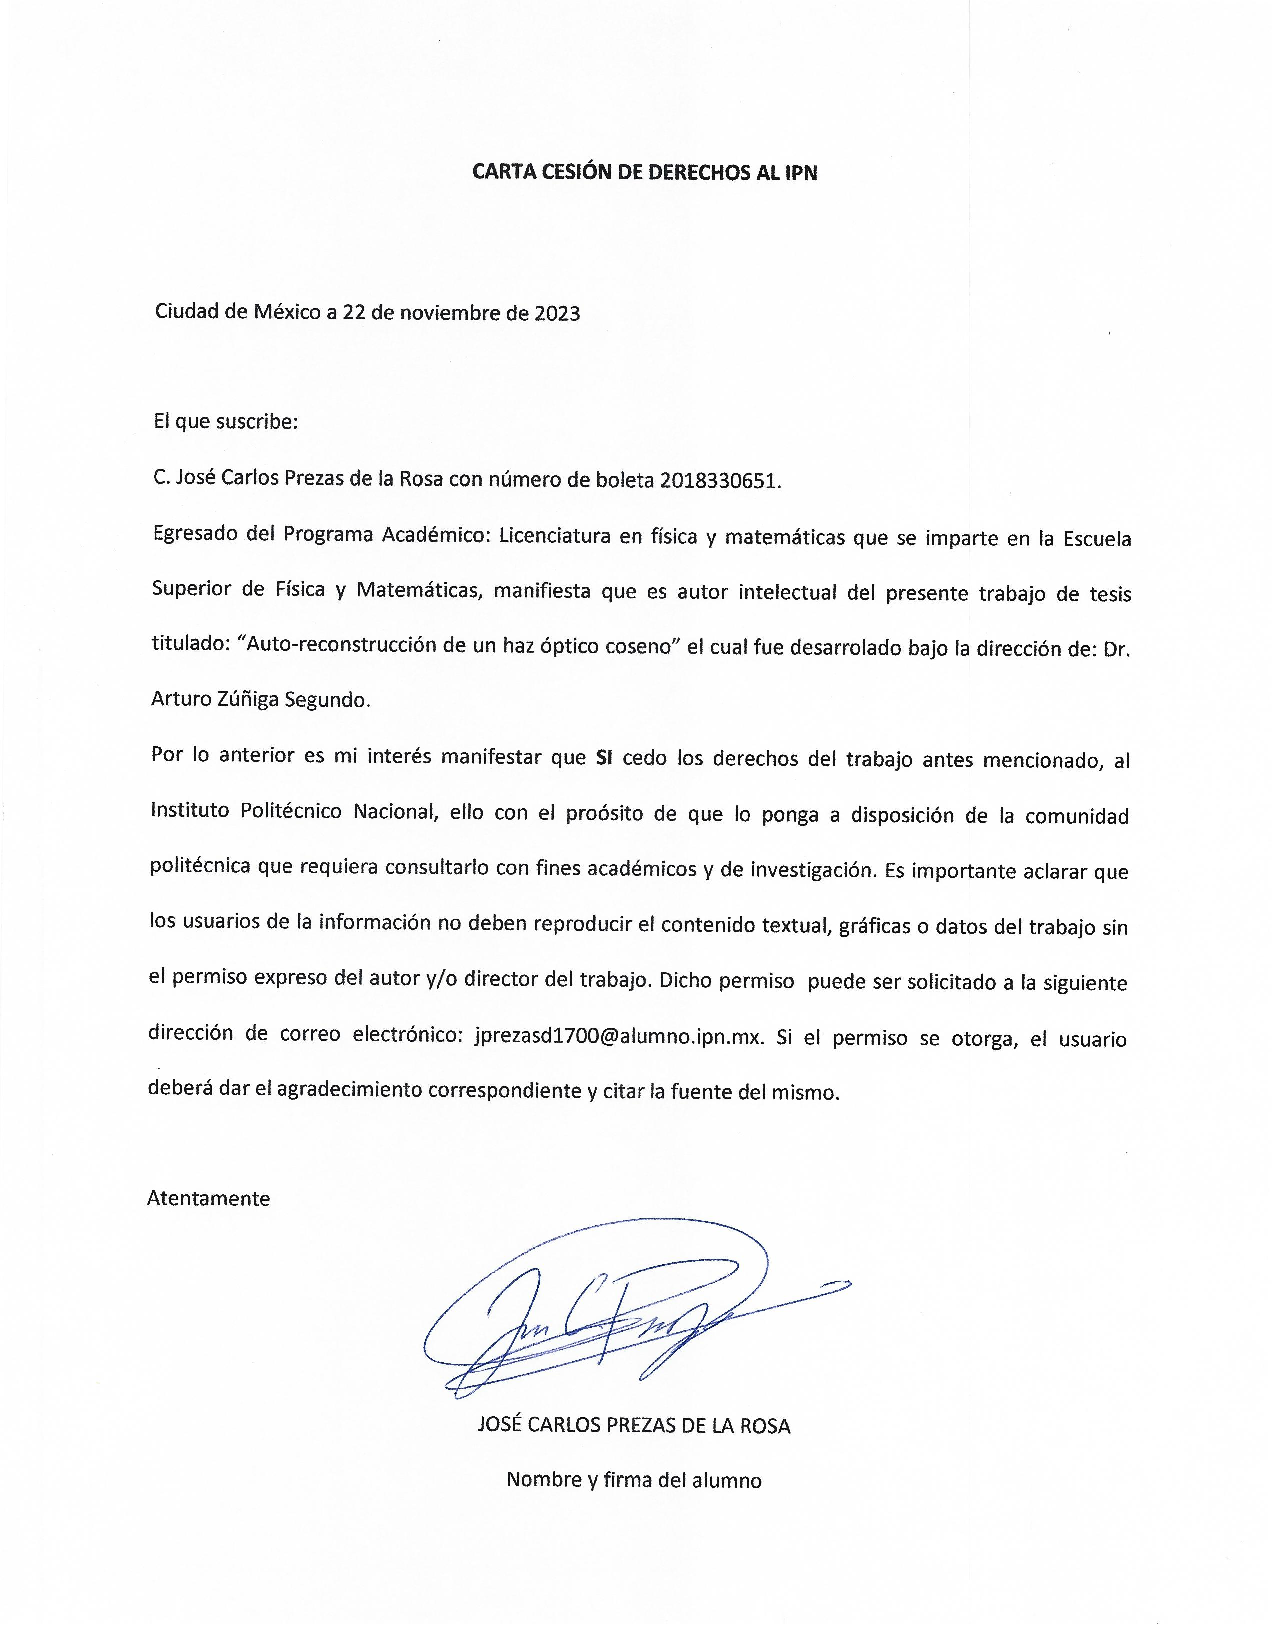
\includepdf[pages=-]{Ces-der-firmado.pdf}
%\includepdf[pages=-]{2023-ESFM-SAC.T-399 José Carlos Prezas de la Rosa - Autorización de impresión.pdf}

  % -*- Mode:TeX -*-
%% This file simply contains the commands that actually generate the table of
%% contents and lists of figures and tables.  You can omit any or all of
%% these files by simply taking out the appropriate command.  For more
%% information on these files, see appendix C.3.3 of the LaTeX manual. 
\tableofcontents
\newpage
%\listoffigures
%\newpage
%\listoftables


\chapter{Introducci\'on}

La mecánica cuántica (MC) es un modelo físico que describe el comportamiento de las formas más pequeñas de la materia a través de la cuantización de la energía. La razón de su existencia se da a partir de fenómenos físicos que la mecánica clásica falla en predecir. Algunos de estos fenómenos son la radiación de cuerpo negro, el efecto fotoeléctrico y el no colapso de los electrones en los átomos.

Un experimento que ilustra la necesidad de un espacio complejo de considerar un espacio vectorial complejo para modelar fenómenos físicos es el de Stern-Gerlach (SG). El experimento consiste en átomos de plata (Ag) disparados a lo largo de dos piezas polares, teniendo una de estas un borde afilado. De los 47 electrones del átomo de plata, uno (5s) no tiene una contraparte simétrica, y genera un momento angular intrínseco. El momento magnético es proporcional al espín, y estos átomos al pasar a lo largo del espacio entre las dos piezas polares experimentarán una fuerza dependiendo de la dirección de su componente $z$. Estos colisionan en una pantalla, donde clásicamente se esperaría una distribución Gaussiana de puntos de choque de los átomos a lo largo de la pantalla. Sin embargo en realidad se observan dos manchas bien distinguidas entre sí. Del experimento se concluye que son solo dos los posibles valores del espín del electrón, sucediendo con la misma probabilidad.

Realizando este experimento de manera secuencial, pero direccionando el campo magnético en la componente $x$ y bloqueamos con una pantalla el haz de átomos con electrones con $S_z^-$. De esta forma asumiríamos que la mitad de los átomos pasando el segundo experimento tendrían una configuración $S_z^+$, $S_x^-$ y la otra mitad
$S_z^+$, $S_x^+$. Para verificar esta hipótesis, se puede realizar un tercer experimento de SG en secuencia, de nueva cuenta generando un campo magnético no homogéneo a lo largo del eje $z$. Si todos los átomos tienen una configuración con $S_z^+$, se esperaría que todos los átomos se vean reflejados en la pantalla superior, sin embargo, este no es el caso. La "selección" de átomos en el segundo experimento de SG destruye cualquier información del primer experimento de SG en la componente $z$. En notación de Dirac, estas posibles combinaciones se pueden escribir como:
\begin{equation}
  \label{1.1}
  \ket{S_x; \pm} = \pm \frac{1}{\sqrt{2}}\ket{S_z; +} + \frac{1}{\sqrt{2}}\ket{S_z; -}\,.
\end{equation}
Esto se puede representar en un espacio vectorial bidimensional complejo. Esta necesidad surge de utilizar la misma base $\ket{S_z; \pm}$ para representar los estados de espín en $y$. El espacio se describe por combinaciones lineales de los vectores base y coeficientes complejos
\begin{equation}
  \label{1.2}
  \ket{S_y; \pm} = \frac{1}{\sqrt{2}}\ket{S_z; +} \pm \frac{i}{\sqrt{2}}\ket{S_z; -}\,.
\end{equation}

% Aquí, ^x y ^p obedecen la relación canónica de conmutación, por lo tanto su espectro no tiene máximo y es continuo (Ver pág. 40 Leonhardt)

El espacio vectorial complejo utilizado tiene una dimensionalidad que depende el sistema físico estudiado. En el caso del experimento de SG previamente considerado, la dimensión es dos. En casos donde las variables son continuas, como es el caso del momento y la posición, estos se describen por espacios de infinita dimensión denominados de Hilbert, cuyos elementos $\ket{\psi}$ se denominan estados, y a las variables se les representa por observables $\hat{A}$, en este caso $\hat{p}$ y $\hat{x}$ para el momento y posición, respectivamente. De la naturaleza de un espacio vectorial, se obtiene el principio de superposición, dados dos estados $\ket{\psi_1}$ y $\ket{\psi_2}$, cualquier combinación lineal $c_1 \ket{\psi_1} + c_2 \ket{\psi_2}$ con $|c_1|^2 + |c_2|^2 = 1$ es también un estado puro del sistema. El principio de superposición explica la interferencia y, de acuerdo a la interpretación probabilista de Max Born, los módulos cuadrados de los coeficientes denotan las probabilidades de que el sistema se encuentre en dicho estado al momento de realizar una medición.

Dos operadores se dicen compatibles si son tales que su conmutación es cero, es decir $[\hat{A}, \hat{B}] = \hat{A}\hat{B} - \hat{B}\hat{A} = 0$, es decir, que el orden de aplicación de los operadores afecta de igual manera a un estado $\hat{A} \hat{B} \ket{\psi} = \hat{B} \hat{A} \ket{\psi}$. Por otro lado, si la diferencia es distinta de cero, se dice que son no compatibles. Este último es el caso de los operadores $\hat{x}$ y momento $\hat{p}$, cuya relación de conmutación es
\begin{equation}
  \label{1.3}
  [\hat{x}, \hat{p}] = i\hbar \hat{I}\,.
\end{equation}

Dado un observable $\hat{A}$, se puede definir un operador $\Delta A \def \hat{A} - \langle \hat{A} \rangle$. El cuadrado del valor esperado de este operador se conoce como la dispersión $\langle (\Delta A)^2 \rangle = \langle \hat{A}^2\rangle  - \langle\hat{A}\rangle^2$. La dispersión se anula cuando el estado tratado es un eigenestado del observable $\hat{A}$. A partir de estas definiciones, para dos observables $\hat{A}$ y $\hat{B}$ y cualquier estado se debe satisfacer la relación de incertidumbre generalizada \cite{Sakurai}
\begin{equation}
  \label{1.4}
  \langle (\Delta A)^2 \rangle \langle (\Delta B)^2 \rangle \geq \frac{1}{4} \left| \left\langle \left[ \hat{A}, \hat{B} \right] \right\rangle  \right|^2 \,.
\end{equation}
% Change of basis and diagonalization theory
Dados dos observables incompatibles $\hat{A}$ y $\hat{B}$ con bases dados por sus eigenestados $\left\{\ket{a}\right\}$ y $\left\{\ket{b}\right\}$ respectivamente, se puede realizar un cambio de representación o base para estudiar cómo están relacionadas estas dos descripciones del espacio de kets. Este cambio de base está dado por una transformación de similitud $\hat{B} = \hat{U}^\dagger \hat{A} \hat{U}$. con $\hat{U}$ un operador unitario llamado matriz de transformación dado por $\hat{U} = \sum_k \ket{b_k}\bra{a_k}$, con $\ket{a_k}$ y $\ket{b_k}$ las bases de los eigenestados de los operadores $\hat{A}$ y $\hat{B}$ respectivamente. La traza de un operador $\hat{A}$ está definida como la suma de los elementos diagonales de la matriz asociada $A$ y es independiente a la representación
\begin{equation}
  \text{Tr}(A) = \sum_a \bra{a}A\ket{a}
\end{equation}
El encontrar la matriz unitaria que diagonaliza $B$ es equivalente a encontrar los eigenvalores y eigenestados del operador $B$ cuyos elementos matriciales en la base $\{\ket{a}\}$ previa a la transformación son conocidos. Conocida la matriz de transformación $U$, se puede construir la transformación unitaria de $A$ $UAU^{-1}$ y se dicen observables unitariamente equivalentes. El conjunto $\{ket{b}\}$ son eigenestados de $UAU^{-1}$ con los mismos eigenvalores que los eigenvalores de $A$, haciendo su espectro idéntico.
% Teoría de matriz de densidad
Los estados cuánticos que describe un ket $\ket{\psi}$ y su respectiva función de onda $\psi$ pueden representar un sistema físico solo si este no está compuesto por más subensembles independientes entre si. A dichos estados se les denomina puros. Si, por el contrario, el sistema físico no puede ser descrito por un estado puro, se utiliza una distribución estadística de estados puros a la que se le denomina estado mixto. Ambos tipos de sistemas se pueden describir usando la matriz de densidad $\hat{\rho}$, que es la forma más general para describir sistemas en la mecánica cuántica\cite{Pena}. Sea $\hat{A}$ un operador cualquiera, el valor esperado de este operador se calcula como $\hat{A} = \text{Tr}\left\{ \hat{\rho} \hat{A} \right\}$. En el caso de un ensemble con varios subensembles descritos por un estado $\ket{i}$, cada uno contribuyendo al sistema con un peso $\omega_i$, el operador de densidad está dado por $\hat{\rho} = \sum_i \omega_i \ket{i} \bra{i}$, lo que en un estado puro $\ket{\psi}$ se reduce a $\hat{\rho} = \ket{\psi}\bra{\psi}$ que recupera la definición de valor esperado de un operador $\hat{A}$ en estados puros dada por $\langle\hat{A}\rangle = \bra{\psi}\hat{A}\ket{\psi}$.
%Ecuación de Schrödinger y necesidad del operador de evolución temporal
Todos los sistemas cuánticos reales están sujetos a una evolución temporal. La ecuación de Schrödinger completa justamente describe la evolución temporal de una función de onda $\psi$
\begin{equation}
  i\hbar\frac{\partial \psi}{\partial t} = -\frac{\hbar^2}{2m}\nabla^2 \psi + V\psi
\end{equation}
Se pueden expresar las soluciones en términos de funciones propias que corresponden al problema estacionario y el potencial $V$ no es función del tiempo. Se expresa entonces la función de onda como una superposición de las ondas monocromáticas que resultan de la solución espacial de la ecuación de onda del problema estacionario $\varphi_n(\mathbf{r})$
\begin{equation}
  \psi(\mathbf{r}, t) = \sum_n c_n e^{-iE_n t/\hbar}\psi_n(\mathbf{r})
\end{equation}
% Evolución temporal de un sistema cuántico
En la notación de Dirac, considere un estado que depende del tiempo cuyo valor $\ket{\psi(t)}$ que se encuentra en el estado $\ket{\psi}(t_0)$ en un tiempo fijo $t_0$. Se relaciona al estado fijo con el dependiente del tiempo a través del operador de evolución temporal como $\ket{\psi(t)} = \hat{U}(t, t_0) \ket{\psi(t_0)}$, que considerando $t_0=0$ se puede simplificar a $\ket{\psi(t)} = \hat{U}(t) \ket{\psi(t_0)}$. La expresión explícita del operador se obtiene construyendola a partir de las propiedades que debe cumplir. El operador debe ser unitario $U^\dagger(t)\hat{U}(t) = 1$, que aplicaciones sucesivas de tiempos $t_1$ y $t_2$ sean equivalentes a la evolución en un tiempo $t_1+t_2$, y que el operador infinitesimal se reduzca a la identidad cuando $dt$ vaya a cero. Resulta de las anteriores consideraciones que el operador es de la form $\hat{U}(t) = 1-\frac{i\hat{H}dt}{\hbar}$, y su ecuación diferencial fundamental es la ecuación de Schrödinger para el operador de evolución temporal.
\begin{equation}
  i\hbar\frac{\partial}{\partial t} \hat{U}(t) = \hat{H}\hat{U}(t)
\end{equation}
Cuando el Hamiltoniano es independiente del tiempo, la solución a esta ecuación está dada por
\begin{equation*}
  \hat{U}(t) = \exp{\left[ \frac{-i\hat{H}t}{\hbar} \right]}
\end{equation*}
% Oscilador armónico simple
\section{Oscilador armónico cuántico}

El oscilador armónico cuántico (OAC) es uno de los pocos modelos que tiene soluciones analíticas en la mecánica cuántica. La cinemática de varios sistemas periódicos y de tipo ondulatorio se puede describir utilizando el modelo del OAC.
Varios potenciales independientes del tiempo $V(x)$ se pueden describir alrededor de un mínimo con una expansión en serie de Taylor
\begin{align*}
  V(x) & = \sum_{n=0}^{\infty} \frac{V^{(n)}}{n!} (x)|_{x_0} (x-x_0)^n \\ &= V(x_0) + \frac{dV}{dx}\Big|_{x_0} (x-x_0) + \frac{1}{2}\frac{d^2V}{dx^2}\Big|_{x_0} (x-x_0)^2 + \dots \,,
\end{align*}
el segundo término se anula por definición de mínimo local. Por formalismo, se puede recorrer el potencial $x = x' + x_0$ para que el potencial en $x_0$ sea $V(x_0) = 0$, eliminando el primer término. Finalmente, el término dominante en la expansión es la segunda derivada
\begin{equation}
  \label{OA.1}
  V(x) = \frac{1}{2}\frac{d^2V(x)}{dx^2}\Big|_{x_0}x^2 \,,
\end{equation}

lo anterior se puede aplicar para un potencial que depende de más dimensiones $V(\mathbf{x})$. Asumiendo que todos los potenciales se han recorrido de manera análoga $x_i \to x_i + x_{oi}$

\begin{equation*}
  V(x_1, \dots, x_N) = \frac{1}{2}\sum_{i=1}^N \sum_{j=1}^N \frac{\partial^2 V}{\partial x_i \partial x_j}\Big|_{0} x_i x_j \,,
\end{equation*}

para hamiltonianos con potenciales cuadráticos, es siempre posible hacer un cambio de coordenadas de la forma

\begin{equation*}
  (x_{1}, \dots, x_N) \to (u_1, \dots, u_N)\,,
\end{equation*}

donde el potencial se desacopla, \textit{i.e.} sin derivadas cruzadas, y se puede describir por $n$ osciladores armónicos individuales

\begin{equation*}
  V(u_1, \dots, u_N) = \frac{1}{2} \sum_{i=1}^{N} \frac{\partial^2 V}{\partial u_i^{2}}\Big|_0 u_i^2\,.
\end{equation*}

Considerando un ejemplo básico de un oscilador armónico clásico, se tienen las ecuaciones clásicas de movimiento

\begin{align}
  m \frac{d^2x}{xt^2} & = -kx \,, \label{OA.2}            \\
  p                   & = m\frac{dx}{dt} \,, \label{OA.3}
\end{align}

con $k$ la constante del resorte, $m$ la masa de la partícula, $x$ el desplazamiento de la posición de equilibrio y $p$ el momento lineal, esto se sustituye en la ecuación estacionaria de Schrödinger, que se debe resolver es:

\begin{equation}
  \label{OA.4}
  -\frac{\hbar^2}{2m}\frac{d^2}{dx^2}\psi(x) + \frac{1}{2}m \omega^2 x^2 \psi(x) = E \psi(x) \,.
\end{equation}

Una partícula en un sistema tiene una energía cinética que corresponde a
\begin{equation*}
  \hat{T} = \frac{\hat{p}^2}{2m}\,,
\end{equation*}

y el hamiltoniano correspondiente está dado por
\begin{equation}
  \hat{H} = \hat{T} + \hat{V} = \frac{\hat{p}^2}{2m} +\frac{1}{2} m\omega^2 \hat{q}^2 \label{OA.5}\,,
\end{equation}

% Following the Loudon method

donde $\omega$ es la frecuencia angular del oscilador clásico.
El problema del oscilador armónico puede ser resuelto de forma analítica (encontrando los eigenvalores y eigenfunciones de la ecuación de Schrödinger) o de forma algebraica, que involucra la introducción de dos operadores $\hat{a}^{\dagger}$ y $\hat{a}$, los operadores escalera de creación y aniquilación, respectivamente, definidos en términos de $\hat{q}$ y $\hat{p}$ como:
% Definido en Sakurai de esta forma

\begin{align}
  \hat{a}^{\dagger} & = (2m\hbar\omega)^{-1/2}(m\omega \hat{q} - i\hat{p})\label{OA.6} \,,   \\
  \hat{a}           & = (2m\hbar \omega)^{-1/2}(m\omega \hat{q} + i \hat{p})\label{OA.7} \,,
\end{align}
el conmutador de estos operadores resulta
\begin{equation}
  \label{OA.8}
  [\hat{a}, \hat{a}^{\dagger}] = \hat{1} \,,
\end{equation}
los operadores no son hermitianos, y como tal no representan una propiedad observable del oscilador. % Loudon

Los productos entre estos dos operadores son
\begin{align}
  \hat{a}^{\dagger}\hat{a} & = \frac{1}{2m\hbar\omega} \left( \hat{p}^2 + m^2\omega^2\hat{q}^2 + im\omega\hat{q}\hat{p} - im\omega\hat{p}\hat{q} \right) \nonumber \\
                           & = \frac{1}{\hbar\omega}\left( \frac{\hat{p}^2}{2m} + \frac{1}{2}m\omega^2\hat{q}^2 +\frac{i\omega}{2} [\hat{q}, \hat{p}] \right)
  \nonumber                                                                                                                                                        \\
                           & = \frac{1}{\hbar\omega} \left( \hat{H} + \frac{i\omega}{2}(i\hbar) \right) \nonumber                                                  \\
                           & = \frac{1}{\hbar\omega} \left( \hat{H} - \frac{1}{2}\hbar\omega \right) \label{OA.9}\,.
\end{align}
A partir del anticonmutador de los operadores (\ref{OA.5}) y (\ref{OA.6}), se obtiene lo siguiente
\begin{align}
  \frac{1}{2}\{ \hat{a},\hat{a}^{\dagger}\} & = \frac{1}{2}\hat{a}\hat{a}^{\dagger} + \frac{1}{2}\hat{a}^{\dagger}\hat{a}                                                \nonumber                             \\
                                            & = \frac{1}{2}\hat{a}\hat{a}^{\dagger} - \frac{1}{2}\hat{a}^{\dagger}\hat{a} +\frac{1}{2}\hat{a}^{\dagger}\hat{a} + \frac{1}{2}\hat{a}^{\dagger}\hat{a} \nonumber \\
                                            & = \frac{1}{2}[\hat{a},\hat{a}^{\dagger}] + \hat{a}^{\dagger}\hat{a}                                                        \nonumber                             \\
                                            & = \frac{1}{2} + \hat{a}^{\dagger}\hat{a} \label{OA.10}\,,
\end{align}

por lo que el de las ecuaciones (\ref{OA.9}) y (\ref{OA.10}) el hamiltoniano (\ref{OA.5}) se puede reescribir como

\begin{equation}
  \label{OA.11}
  \hat{H} = \hbar \omega \left(\hat{a} \hat{a}^{\dagger} + \frac{1}{2}\right) = \frac{1}{2}\hbar \omega \left( \hat{a}\hat{a}^{\dagger} + \hat{a}^{\dagger}\hat{a} \right) \,.
\end{equation}

Se introduce también el operador número, definido como
\begin{equation}
  \label{OA.12}
  \hat{n} = \hat{a}^{\dagger} \hat{a}\,,
\end{equation}
y el hamiltoniano (\ref{OA.11}) se puede escribir también como

\begin{equation}
  \label{OA.13}
  \hat{H} = \hbar \omega \left(\hat{n} + \frac{1}{2}\right)\,,
\end{equation}
cuya ecuación de eigenvalores de la energía es
\begin{equation}
  \label{OA.14}
  \hat{H} \ket{n} = E_n\ket{n} \,,
\end{equation}
donde $\ket{n}$ es un eigenestado del OAC con eigenvalor $E_n$. A partir de ciertas operaciones algebráicas, se puede encontrar otra ecuación de eigenvalores a partir de la anterior multiplicando $\hat{a}$ por la izquierda, y resulta de la forma
\begin{align*}
  \hat{H} \hat{a}\ket{n} & = \hbar\omega\left(\hat{a}^{\dagger}\hat{a}+\frac{1}{2}\right)\hat{a}\ket{n} = \hbar\omega\left(\hat{a}\hat{a}^{\dagger}+\hat{a}^{\dagger}\hat{a}-\hat{a}\hat{a}^{\dagger}+\frac{1}{2}\right)\hat{a}\ket{n} \\
                         & = \hbar\omega\left(\hat{a}\hat{a}^{\dagger}-\left[\hat{a},\hat{a}^{\dagger}\right]+\frac{1}{2}\right)\hat{a}\ket{n} = \hbar\omega\left(\hat{a}\hat{a}^{\dagger}-1+\frac{1}{2}\right)\hat{a}\ket{n}          \\
                         & = \hbar\omega\left(\hat{a}\hat{a}^{\dagger}\hat{a}-\hat{a}+\frac{1}{2}\hat{a}\right)\ket{n} = \hat{a}\hbar\omega\left(\hat{a}^{\dagger}\hat{a}+\frac{1}{2}-1\right)\ket{n}                                  \\
                         & = \hat{a}\left(\hbar\omega\left(\hat{n}+\frac{1}{2}\right)-\hbar\omega\right)\ket{n} = \hat{a}\left(\hat{H}-\hbar\omega\right)\ket{n} = \left(E_{n}-\hbar\omega\right)\hat{a}\ket{n}\,,
\end{align*}
donde $\hat{a}\ket{n}$ es también un eigenestado del sistema, pero ahora con un valor propio de energía $E_n - \hbar\omega$, los cuales se denotarán como $\ket{n-1}$ y $E_{n-1}$ respectivamente. Así, la nueva ecuación de eigenvalores es
\begin{equation}
  \label{OA.15}
  \hat{H}\, \hat{a}\ket{n} = E_{n-1}\, \hat{a}\ket{n}\,,
\end{equation} % Citar a Loudon para este procedimiento
de manera similar, pero ahora aplicando el operador $\hat{a}^{\dagger}$ por la izquierda, se llega a la ecuación
\begin{equation}
  \label{OA.16}
  \hat{H} \,\hat{a}^{\dagger}\ket{n} = E_{n+1}\, \hat{a}^{\dagger}\ket{n}\,.
\end{equation}
Los operadores escalera nos permiten conocer el resto de los valores de la energía del oscilador armónico una vez conocido $E_n$, estos valores varían en incrementos de $\hbar\omega$. Debido a que no puede haber un estado con energía negativa, se propone un estado $\ket{0}$, llamado estado base, al que corresponda una energía mínima $E_0$, y con la propiedad:
\begin{equation}
  \label{OA.17}
  \hat{a}\ket{0} = 0\,.
\end{equation}
A partir de esta propiedad se determina que $E_0 = \frac{1}{2}\hbar\omega$ y en general
\begin{equation}
  \label{OA.18}
  E_n = \left( n + \frac{1}{2} \right) \hbar\omega, \quad n\in\mathbf{N}\,.
\end{equation}
% ============================
% ============================
% ============================
% Add explanation of how the cavity modes of EM field expansion = harmonic oscillator = why problems reduce to the harmonic oscillator (what properties let us do that simplification)
% ============================
% ============================
% ============================
Los estados número son eigenestados simultáneos del operador hamiltoniano (\ref{OA.13}) y del operador número (\ref{OA.12}), por lo que tienen una base de eigenvectores en común, donde
\begin{equation}
  \label{OA.19}
  \hat{n}\ket{n} = n\ket{n}\,.
\end{equation}

Los estados se pueden normalizar utilizando las condiciones
\begin{equation}
  \label{OA.20}
  \langle n\vert m\rangle = \delta_{n,m}
\end{equation}
y los coeficientes de normalización para la aplicación de los operadores escalón resultan
\begin{align}
  \hat{a}\ket{n}           & = \sqrt{n} \ket{n-1} \,,\label{OA.21}   \\
  \hat{a}^{\dagger}\ket{n} & = \sqrt{n+1} \ket{n+1} \,.\label{OA.22}
\end{align}

Los operadores $\hat{a}^{\dagger}$ y $\hat{a}$ no son hermitianos, por lo que no representan alguna magnitud f\'isica observable. Es conveniente entonces definir, a partir de la definición de operadores posición $\hat{q}$ y momento $\hat{p}$ generalizado en su forma adimensional utilizados en la expresión del Hamiltoniano del oscilador armónico, los operadores de cuadratura \cite{Loudon}

\begin{equation}
  \label{OA.23}
  \hat{X} = \sqrt{\frac{m\omega}{2\hbar}} \, \hat{q} = \frac{1}{2}\left( \hat{a} + \hat{a}^{\dagger} \right)\,,
\end{equation}
\begin{equation}
  \label{OA.24}
  \hat{Y} = \frac{1}{\sqrt{2m\hbar\omega}} \, \hat{p} = \frac{i}{2}\left( \hat{a}^{\dagger} - \hat{a} \right)\,,
\end{equation}
los operadores escalera en términos de los de cuadratura son
\begin{equation}
  \label{OA.25}
  \hat{a} = \hat{X} + i{Y}\,,
\end{equation}
\begin{equation}
  \label{OA.26}
  \hat{a}^{\dagger} = \hat{X} - i\hat{Y}\,,
\end{equation}
la relación de conmutación entre estos operadores es
\begin{equation}
  \label{OA.27}
  \left[ \hat{X}, \hat{Y} \right] = \frac{i}{2}
\end{equation}
y su relación de incertidumbre es:
\begin{equation}
  \label{OA.28}
  \langle (\Delta X)^2 \rangle \langle (\Delta Y)^2 \rangle \geq \frac{1}{16}\,,
\end{equation}
con estos también se puede expresar el Hamiltoniano del oscilador armónico simple
\begin{equation}
  \label{OA.29}
  \hat{H} = \hbar \omega \left( \hat{X}^2 + \hat{Y}^2 \right)\,.
\end{equation}
% Agregar teoría de fasores e incertidumbre de Fox cap 7.3
\chapter{Cuantizaci\'on del campo electromagn\'etico}

\section{Ecuaciones de Maxwell}

Las variables de campo eléctrico $\mathbf{E}$, y magnético $\mathbf{H}$, así como el de desplazamiento $\mathbf{D}$ el de inducción magnética $\mathbf{B}$ se pueden tratar como observables, cuyos valores esperados son el promedio de un ensemble cuántico de campos, es decir, se pueden representar por operadores Hermitianos $\hat{\mathbf{E}}$, $\hat{\mathbf{H}}$, $\hat{\mathbf{D}}$ y $\hat{\mathbf{B}}$ respectivamente. La linealidad de las ecuaciones de Maxwell permiten que obedezcan la interpretación estadística de Max Born, viendo que el promedio de cada una de las leyes se reduce a las leyes de Maxwell aplicadas a los promedios. Por el mismo argumento de linealidad, las ecuaciones constitutivas son válidas para estos mismos operadores, y se tiene (en SI) $\mathbf{D} = \epsilon_0 \epsilon \mathbf{E}$ y $\mathbf{B} = \mu_0 \mu \mathbf{H}$ con $\epsilon_0 \mu_0 = c^{-2}$.
Las ecuaciones de Maxwell rigen el comportamiento de los campos electromagnéticos clásicos y cuánticos.
\begin{align}
  \nabla \cdot \hat{\mathbf{B}}  & = 0 \,,                                              \label{EM.1}                 \\
  \nabla \times \hat{\mathbf{E}} & = - \frac{1}{c} \frac{\partial \hat{\mathbf{B}}}{\partial t}\,,      \label{EM.2} \\
  \nabla \cdot \hat{\mathbf{D}}  & = 0 \,,                                        \label{EM.3}                       \\
  \nabla \times \hat{\mathbf{B}} & = \frac{1}{c}
  \frac{\partial \hat{\mathbf{E}}}{\partial t}\,, \label{EM.4}
\end{align}
donde todos los campos son dependientes de la posición $\mathbf{r}$ y del tiempo $t$\footnote{Se utilizan unidades de CGS a lo largo de este desarrollo.}

Se define el operador de campo vectorial $\hat{\mathbf{A}}$ de manera que cumpla
\begin{align}
  \hat{\mathbf{E}} & = -\frac{1}{c}\frac{\partial \hat{\mathbf{A}}}{\partial t}, \label{EM.5} \\
  \hat{\mathbf{B}} & = \nabla \times \hat{\mathbf{A}}\,.\label{EM.6}
\end{align}
% Justificación de la elección del Gauge de Coulomb
Se elige entonces el gauge de Coulomb, haciendo el potencial escalar cero y el potencial vectorial $\hat{\mathbf{A}}$ tal que satisfaga la condición de transversalidad $\nabla \cdot \hat{\mathbf{A}} = 0$ \footnote{El presente desarrollo se realiza en el dominio no relativista \cite{Agarwal_2012}.}, haciendo que la primera ecuación de Maxwell (\ref{EM.4}) se cumpla de manera directa. Sustituyendo las ecuaciones (\ref{EM.5}) y (\ref{EM.6})
en la ecuaci\'on de Ampere-Maxwell (\ref{EM.4})
\begin{align}
  \label{EM.7}
  \nabla \times \hat{\mathbf{B}} = \nabla \times \left(\nabla\times\hat{\mathbf{A}}\right)
  =\frac{1}{c}\frac{\partial \hat{\mathbf{E}}}{\partial t} = \frac{1}{c}\frac{\partial}{\partial t} \left(-\frac{1}{c}\frac{\partial\hat{\mathbf{A}}}{\partial t}\right) = -\frac{1}{c^{2}}\frac{\partial^{2}\hat{\mathbf{A}}}{\partial t^{2}} \,,
\end{align}
obteniendo la ecuación de onda electromagnética
\begin{equation}
  \label{EM.8}
  \nabla^2 \hat{\mathbf{A}} = \frac{1}{c^2} \frac{\partial^2 \hat{\mathbf{A}}}{\partial t^2}\,,
\end{equation}
% Demostrar que los operadores de campo electromagnético son Hermitianos
la conocida solución particular de la onda plana se puede obtener por el método de separación de variables y se reduce al resultado de la onda plana
\begin{equation}
  \label{EM.9}
  \hat{\mathbf{A}}_k = \hat{c}_k \mathbf{e}^{(\lambda)}\exp{(i\mathbf{k}\cdot \mathbf{r})}\exp{(-i\omega_k t)} = \hat{c}_{k}\mathbf{u}_{k\lambda}(\mathbf{r}) \exp{(-i\omega_k t)} \,,
\end{equation}
con $\mathbf{k} = (k_x, k_y, k_z)$ el vector de número de onda, cuya magnitud está dada por $k = 2\pi/\lambda$ \cite{Riley}, y $\hat{\mathbf{u}}_{k\lambda}(\mathbf{r}) = \hat{\mathbf{e}}^{(\lambda)} \exp{(i\mathbf{k}\cdot \mathbf{r})}$ con $\hat{\mathbf{e}}^{(\lambda)}$ el vector de polarización, donde $\lambda=1,2$ es el índice de polarización \cite{Walls}.

De la teoría de Sturm-Liouville, al definir condiciones de frontera para nuestras coordenadas espaciales, se define un espacio de Hilbert cuyos elementos $\mathbf{u}(\mathbf{r})$ son funciones diferenciables y que satisfacen anularse en las fronteras dadas. La ecuación de eigenvalores se escribe como \cite{Arfken}:
\begin{equation}
  \label{EM.10}
  \mathcal{L} \hat{\mathbf{A}} = \left( \frac{\partial^2}{\partial x^2} + \frac{\partial^2}{\partial y^2} + \frac{\partial^2}{\partial z^2} \right) \hat{\mathbf{A}} = (k_x^2 + k_y^2 + k_z^2) \hat{\mathbf{A}} \,,
\end{equation}
con
\begin{equation}
  \label{EM.11}
  \mathcal{L} = \frac{\partial^2}{\partial x^2} + \frac{\partial^2}{\partial y^2} + \frac{\partial^2}{\partial z^2} \,.
\end{equation}
La solución general se puede obtener a partir de una superposición de las $k$-ésimas soluciones particulares. A su vez, esta superposición de soluciones se puede separar en dos sumandos de acuerdo a la magnitud de las frecuencias angulares \cite{Riley}. El campo electromagnético se describe entonces restringido a un volumen cúbico en el espacio y el potencial vectorial se expande en términos del conjunto discreto las funciones de modo ortogonales del espacio de Hilbert definido por el \textit{ansatz} (\ref{EM.9}). Separando los términos en las amplitudes incidentes (amplitudes que varían de acuerdo a $e^{-i\omega_k t}$ con $\omega>0$) y reflejadas (amplitudes que varían como $e^{i\omega_k t }$ y $\mathbf{A}^{(-)} = (\mathbf{A}^{(+)})^*$) % Usando la terminología de Griffiths Quantum Mechanics 3rd ed para la solución del pozo finito 
\begin{equation}
  \label{EM.12}
  \mathbf{A} = \mathbf{A}^{(+)} + \mathbf{A}^{(-)} = \sum_{k,\lambda} \left( \hat{c}_{k} \mathbf{u}_{k\lambda} (\mathbf{r})e^{-i\omega_k t} +  \hat{c}_{k}^* \mathbf{u}_{k\lambda}^* (\mathbf{r})e^{i\omega_{k} t} \right) \,,
\end{equation}
nos enfocaremos solo en los términos de amplitudes incidentes, las cuales deben de cumplir, además de ser solución a la ecuación de onda, con la condición de transversalidad
\begin{equation}
  \label{EM.13}
  \nabla \cdot \mathbf{u}(\mathbf{r}) = 0 \,,
\end{equation}
lo cual se cumple al momento de asignarle un vector de polarización $\mathbf{\hat{e}}^{(\lambda)}$ perpendicular a $\mathbf{k}$. A su vez las funciones forman un conjunto ortogonal bajo el producto interno del espacio de Hilbert. Se establecen condiciones de frontera periódicas que corresponden a modos de vibración que llevan a ondas estacionarias en un volúmen cúbico de paredes reflejantes de lados de longitud $L$. De esta condición de ortogonalidad
\begin{equation*}
  \int_V \exp{(i\mathbf{k}\cdot\mathbf{r})} \exp{(-i\mathbf{k}\cdot\mathbf{r})} d\mathbf{r}
  =  \int_V d\mathbf{r}
  =  L^3 = V \,,
\end{equation*}
\begin{equation}
  \label{EM.14}
  \int_V \mathbf{u}^{*}_k(\mathbf{r}) \mathbf{u}_{k'}(\mathbf{r}) d\mathbf{r} = L^3\delta_{kk'} \,.
\end{equation}
Así, las funciones de onda se escriben como
\begin{equation}
  \label{EM.15}
  \mathbf{u}_{k\lambda}(\mathbf{r}) = \mathbf{\hat{e}}_{k\lambda} \exp\left({i\mathbf{k}\cdot \mathbf{r}}\right) \,.
\end{equation}
El vector de propagación $\mathbf{k}$ en coordenadas cartesianas toma los valores por entrada
\begin{equation}
  \label{EM.16}
  k_i = \frac{2\pi n_i}{L}, \quad \text{con } i=x,y,z , \quad n_i = 0, \pm1, \pm 2, \dots
\end{equation}
La densidad de energía del campo electromagnético está dada por $u = \mathbf{E} \cdot \mathbf{D} + \mathbf{B} \cdot \mathbf{E}$ en SI. Considerando el vacío como medio y ningúna fuente, se puede reescribir como $u = \mathbf{E}^2 + \mathbf{B}^2$ (SI). Transformando a unidades CGS, se tiene $\mathbf{E} \to \mathbf{E}/\sqrt{4\pi \varepsilon_0}$ y $\mathbf{B} \to \sqrt{\frac{\mu_0}{4\pi}}\mathbf{B}$, y como $\mu_0=1$ y $\epsilon_0 = 1$ en CGS, la energía electromagnética dentro de un volumen es
\begin{equation}
  \label{EM.17}
  U = \frac{1}{8\pi}\int_V \left[ \mathbf{E}^2(\mathbf{r}, t) + \mathbf{B}^2(\mathbf{r}, t) \right] d\mathbf{r} \,.
\end{equation}
y en forma de operador se expresa con el Hamiltoniano
\begin{equation}
  \label{EM.17H}
  \hat{H} = \frac{1}{8\pi}\int_V \left[ \hat{\mathbf{E}}^2(\mathbf{r}, t) + \hat{\mathbf{B}}^2(\mathbf{r}, t) \right] d\mathbf{r} \,.
\end{equation}
El campo magnético y la inducción magnética se calculan en términos del conjunto de funciones ortonormales $\mathbf{u}_k(\mathbf{r})$ a partir del campo vectorial $\hat{\mathbf{A}}(\mathbf{r}, t)$
\begin{align*}
  \hat{\mathbf{E}}           & = -\frac{1}{c} \frac{\partial \hat{\mathbf{A}}}{\partial t}                                                                                                                                                         \\
                             & =-\frac{1}{c}\left[ \frac{\partial \hat{\mathbf{A}}^{(+)}}{\partial t} + \frac{\partial \mathbf{A}^{(-)}}{\partial t} \right]                                                                                       \\
                             & = -\frac{1}{c} \sum_{k,\lambda} \left[ -i\omega_{k}\hat{c}_{k} \mathbf{u}_{k\lambda} (\mathbf{r})e^{-i\omega_k t} +  i\omega_{k}\hat{c}_{k}^* \mathbf{u}_{k\lambda}^* (\mathbf{r})e^{i\omega_{k} t} \right] \,,     \\
  c^2 \vert\mathbf{E}\vert^2 & = c^2 \mathbf{E} \cdot \mathbf{E}                                                                                                                                                                                   \\
                             & = \sum_{k,\lambda}\sum_{k',\lambda'}\left(-i\omega_{k}\hat{c}_{k}\mathbf{u}_{k\lambda} (\mathbf{r})e^{-i\omega_{k}t} + i \omega_{k} c^{*}_{k}\mathbf{u}^{*}_{k\lambda}(\mathbf{r})e^{i\omega_{k}t} \right)\cdot     \\
                             & \cdot \left(-i\omega_{k'}\hat{c}_{k'}\mathbf{u}_{k'\lambda} (\mathbf{r})e^{-i\omega_{k'}t} + i \omega_{k'} \hat{c}^{*}_{k}\mathbf{u}^{*}_{k'\lambda'}(\mathbf{r})e^{i\omega_{k'}t} \right)                          \\
                             & = \sum_{k,\lambda} \Big[ \left(-i\omega_{k}\hat{c}_{k} \mathbf{u}_{k\lambda} (\mathbf{r})e^{-i\omega_k t}\right)\cdot \left( i\omega_{k}\hat{c}_{k}^* \mathbf{u}_{k\lambda}^* (\mathbf{r})e^{i\omega_{k} t} \right) \\
                             & +  \left(i\omega_{k}\hat{c}_{k}^* \mathbf{u}_{k\lambda} (\mathbf{r})e^{i\omega_{k} t}\right)\cdot \left(-i\omega_{k}\hat{c}_{k} \mathbf{u}_{k\lambda}^* (\mathbf{r})e^{-i\omega_k t}\right) \Big],
\end{align*}
entonces
\begin{equation}
  \label{EM.18}
  \hat{\mathbf{E}}^2 = \frac{2}{c^2}\sum_{k,\lambda} \omega_{k}^2  |\mathbf{u}(\mathbf{r})|^2 \left( \hat{c}_{k} \hat{c}_{k}^* + \hat{c}_{k}^* \hat{c}_{k} \right) \,.
\end{equation}
Para el campo magnético, se selecciona la dirección de polarización del campo eléctrico, analizando solamente su carácter vectorial
$\mathbf{e}^{\lambda}= \mathbf{\hat{\textnormal{\bfseries\i}}}$, entonces
\begin{equation*}
  \mathbf{B} = \mathbf{\hat{\textnormal{\bfseries\j}}} \left( \frac{\partial}{\partial z} A_x - \frac{\partial}{\partial x} A_z \right)
\end{equation*}
pero como la dirección de polarización es en $\mathbf{\hat{\textnormal{\bfseries\i}}}$, solo la componente de $A_x$ es distinta de cero y
\begin{equation*}
  \mathbf{B} = \mathbf{\hat{\textnormal{\bfseries\j}}} \frac{\partial}{\partial z} A_x
\end{equation*}
como
\begin{equation*}
  \frac{\partial \mathbf{u}_{k\lambda}(\mathbf{r})}{\partial z} = i k_z \mathbf{u}_{k\lambda}(\mathbf{r})
\end{equation*}
y
\begin{equation*}
  \frac{\partial \mathbf{u}^{*}_{k\lambda}(\mathbf{r})}{\partial z} = -i k_z \mathbf{u}^{*}_{k\lambda}(\mathbf{r}).
\end{equation*}
\begin{equation*}
  \hat{\mathbf{B}} = \mathbf{\hat{\textnormal{\bfseries\j}}} \sum_{k,\lambda} \left( i k_z \hat{c}_{k} \mathbf{u}_{k\lambda}(\mathbf{r})e^{-i\omega_{k} t} - i k_z \hat{c}_{k}^* \mathbf{u}_{k\lambda}^*(\mathbf{r})e^{i\omega_{k} t}  \right)
\end{equation*}
Calculando su norma al cuadrado usando el producto punto para complejos
\begin{align*}
  \hat{\mathbf{B}}^2 & = \sum_{k,\lambda} \Big[ \left(ik_z \hat{c}_{k} \mathbf{u}_{k\lambda}(\mathbf{r})e^{-i\omega_{k} t}\right)\left(-ik_z \hat{c}_{k}^{*} \mathbf{u}_{k\lambda}^*(\mathbf{r})e^{i\omega_{k} t} \right) \\
                     & + \left(-ik_z \hat{c}_{k}^{*} \mathbf{u}_{k\lambda}^*(\mathbf{r})e^{i\omega_{k} t} \right)  \left(ik_z \hat{c}_{k} \mathbf{u}_{k\lambda}(\mathbf{r})e^{-i\omega_{k} t}\right) \Big]                \\
                     & = 2 \sum_{k,\lambda} k_z^2 |\mathbf{u}(\mathbf{r})|^2 \left( \hat{c}_{k} \hat{c}_{k}^* + \hat{c}_{k}^* \hat{c}_{k} \right) \,.
\end{align*}
Utilizando los operadores de cuadratura $\hat{X}$ y $\hat{Y}$ previamente definidos, se puede reescribir el campo eléctrico. Usando $\mathbf{u}_{k\lambda}(\mathbf{r})e^{-i\omega_k t} = \mathbf{e}_{k\lambda} e^{\mathbf{k}\cdot\mathbf{r}-i\omega_k t}$ se obtiene
\begin{equation*}
  \mathbf{E} = i \sum_{k,\lambda} \left( \frac{8\hbar \pi \omega_k}{V} \right)^{1/2} \mathbf{e}_{k\lambda} \left[ \hat{X}\cos(\mathbf{k}\cdot\mathbf{r} - \omega t) + \hat{Y}\sen(\mathbf{k}\cdot\mathbf{r} - \omega t) \right]
\end{equation*}
Las variables canónicas $\hat{X}$ y $\hat{Y}$ se pueden interpretar como amplitudes de las cuadraturas en las que se descompone el campo eléctrico. \cite{Mandel}
En nuestro eje coordenado, la propagación de la onda electromagnética se de en la dirección $\mathbf{\hat{\textnormal{\bfseries k}}}$, por lo que $|\mathbf{k}| = k = k_z$. Además $\omega_k = kc$ y se obtiene
\begin{equation}
  \label{EM.19}
  \hat{\mathbf{B}}^2 = 2 \sum_{k,\lambda} \frac{\omega_k^2}{c^2}  |\mathbf{u}(\mathbf{r})|^2 \left( \hat{c}_{k} \hat{c}_{k}^* + \hat{c}_{k}^* \hat{c}_{k} \right) \,,
\end{equation}
sustituyendo en la expresión del Hamiltoniano (\ref{EM.17H})
\begin{align*}
  \hat{H} & = \frac{1}{8\pi} \Bigg[ \int_V \left( 2\sum_{k,\lambda} \frac{\omega_{k\lambda}^2}{c^2}  |\mathbf{u}_{k\lambda}(\mathbf{r})|^2 \left( \hat{c}_{k} \hat{c}_{k}^* + \hat{c}_{k}^* \hat{c}_{k} \right) \right) d\mathbf{r} \\ &+ \int_V \left( 2 \sum_{k,\lambda} \frac{\omega_{k\lambda}^2}{c^2} |\mathbf{u}_{k\lambda}(\mathbf{r})|^2 \left( \hat{c}_{k} \hat{c}_{k}^* + \hat{c}_{k}^* \hat{c}_{k} \right) \right)d\mathbf{r} \Bigg] \\
          & = \frac{1}{2\pi c^2} \sum_{k,\lambda} \omega_{k\lambda}^2 \left( \hat{c}_{k} \hat{c}_{k}^* + \hat{c}_{k}^* \hat{c}_{k} \right) \int_V |\mathbf{u}_{k\lambda}^2(\mathbf{r})|^2 d\mathbf{r} \,,
\end{align*}
donde por la condición de ortogonalidad
\begin{equation}
  \label{EM.20}
  \hat{H} = \frac{V}{2\pi c^2}\sum_{k,\lambda} \omega_{k\lambda}^2 \left( \hat{c}_{k} \hat{c}_{k}^* + \hat{c}_{k}^* \hat{c}_{k} \right) \,,
\end{equation}
ahora si consideramos
\begin{equation}
  \label{EM.21}
  \hat{c}_{k} = \sqrt{\frac{\pi c^{2}\hbar}{\omega_{k}V}} \hat{a}_{k}\,,
\end{equation}
la ecuaci\'on (\ref{EM.20}) se convierte en:
\begin{align*}
  \hat{H} & = \frac{V}{2\pi c^2}\sum_{k} \omega_{k}^2 \frac{\pi c^{2}\hbar}{\omega_{k}V}\left(\hat{a}_{k}\hat{a}^{*}_{k} + \hat{a}_{k}^{*} \hat{a}_{k} \right) = \frac{V}{2\pi c^2}\sum_{k} \omega_{k}^2 \frac{\pi c^{2}\hbar}{\omega_{k}V}\left(\hat{a}_{k}\hat{a}^{*}_{k} + \hat{a}_{k}^{*} \hat{a}_{k} \right) \\
\end{align*}
\begin{equation}
  \label{EM.22}
  \hat{H} = \sum_{k} \frac{\hbar\omega_{k}}{2}\left(\hat{a}_{k}\hat{a}^{*}_{k} + \hat{a}_{k}^{*} \hat{a}_{k} \right)
\end{equation}
En orden de cuantizar el campo electromagnético, se escogen $\hat{a}_{k}$ y $\hat{a}^{*}_{k}$ como los operadores de aniquilaci\'on $\hat{a}_{k}$ y creaci\'on $\hat{a}^{\dagger}_{k}$ para cada modo del campo $k$. Como el objeto de estudio son fotones, el conmutador de bosones es el que se debe seguir
\begin{equation*}
  [\hat{a}_k, \hat{a}^{\dagger}_{k'}] = [\hat{a}^{\dagger}_k, \hat{a}_{k'}] = 0, \quad [\hat{a}_k, \hat{a}_{k'}^{\dagger}] = \delta_{kk'} \,.
\end{equation*}
\iffalse
  Los operadores de campo electromagnético $\mathbf{E}$, $\mathbf{B}$ y $\vec{A}$ son Hermitianos (demostrar, Agarwal), por lo que se pueden descomponer al campo $\mathbf{A}$ en la suma del campo $\mathbf{A}^{(+)}$ que contiene todas las frecuencias positivas  y su complejo conjugado $\mathbf{A}^{(-)}$. (Walls)

  Considere primero una onda electromagnética, descompuesta en dos términos de esta forma
  \begin{equation*}
    \mathbf{E}^{(+)} = \hat{\varepsilon} E_0 \exp{\left(i\vec{k}\cdot \vec{r} - i\omega_k t\right)}, \omega > 0
  \end{equation*}
  Donde $k = |\vec{k}| = \omega_k/c$y $\hat{\varepsilon}$ es el vector de polarización del campo electromagnético, el cual es ortogonal a la dirección de propagación y es perpendicular a la dirección de propagación $\vec{k}$. Hay dos direcciones de polarización, y se denota por el índice $s$ con valores $1$, $2$. De esta forma se tiene que el vector de polarización depende de dos índices y $\vec{\varepsilon} = \vec{\varepsilon}_{\vec{k},s}$ En términos del operador campo vectorial $\mathbf{A}$ del gauge de Coulomb
  \begin{align*}
    \mathbf{A}^{(+)} & = -\frac{1}{c}\frac{\partial \mathbf{A}}{dt} \mathbf{E}^{(+)}                                                           \\
                     & = -\frac{(-i\omega_k)}{c}\hat{\varepsilon} E_0 \exp{\left(i\vec{k}\cdot \vec{r} - i\omega_k t\right)}, \quad \omega > 0 \\
                     & = \hat{\varepsilon} A_0 \exp{\left(i\vec{k}\cdot \vec{r} - i\omega_k t\right)}, \quad \omega > 0
  \end{align*}
  Donde $A_0=\frac{(i\omega_k)}{c}E_0$. Esto nos permite construir la solución de onda plana de la ecuación de onda del campo vectorial $\mathbf{A}$. (Agarwal) Al término $\hat{\varepsilon} \exp{\left(i\vec{k}\cdot \vec{r}\right)}$ se le denomina función de modo y se le denotará por $\hat{u} = \hat{u}(\vec{r})$, satisfacen la ecuación de onda y de transversalidad al igual que $\mathbf{A}$. (Walls).

  Se establecen ahora condiciones de frontera, considerando un volumen cúbico de lados de longitud $L$ y periodicidad. Estas condiciones corresponden a modos de ondas viajeras que en paredes reflejantes se pueden describir como ondas estacionarias. Las funciones de modo forman un conjunto ortonormal completo con estas condiciones, es decir
  \begin{equation*}
    \int_V \hat{u}_k^{*}(\vec{r}) u_{k'} \vec{r} d^3 r = \delta_{kk'}
  \end{equation*}
  En coordenadas cartesianas, de las condiciones de frontera establecen los valores de $k_\alpha$ con $\alpha = x,y,z$.
  \begin{equation*}
    k_i = \frac{2\pi n_i}{L}, \quad n_i = 0, \pm1, \pm2, \dots
  \end{equation*}
  La suma en las direcciones de propagación $\vec{k}$ todos los modos y las dos direcciones de polarización $s$, denotando $V = L^3$, se tiene
  \begin{align*}
    \mathbf{A}^{(+)} & = \sum_{\vec{k}, s} \frac{A_{\vec{k}s}}{\sqrt{V}} \hat{\varepsilon}_{\vec{k}s} \exp{ \left( i\vec{k}\cdot\vec{r} - i \omega_k t \right) } \\
                     & = \sum_{\vec{k},s} \frac{A_{\vec{k}s}}{\sqrt{V}} \hat{u} \exp{\left( - i \omega_k t \right)}
  \end{align*}
  Así, el potencial vectorial es
  \begin{equation*}
    \mathbf{A}(\vec{r}, t) = \sum_{\vec{k}, s} \left( \frac{\hbar}{2\omega_k \epsilon_0} \right)^{1/2} \left( \hat{a}^{\dagger} \hat{u}_k(\vec{r}) e^{-i\omega_k} t + \hat{a} \hat{u}_k(\vec{r})^{*} e^{i\omega_k} t \right)
  \end{equation*}
  y el campo eléctrico es entonces
  \begin{equation*}
    \mathbf{E}(\vec{r}, t) = i\sum_{\vec{k}, s} \left( \frac{\hbar\omega_k}{2\epsilon_0} \right)^{1/2} \left( \hat{a}^{\dagger} \hat{u}_k(\vec{r}) e^{-i\omega_k} t - \hat{a} \hat{u}_k(\vec{r})^{*} e^{i\omega_k} t \right)
  \end{equation*}
  Esto iría en otro capítulo?
  Los coeficientes adminesionales de Fourier son números complejos. En orden de cuantizar el campo electromagnético, se escogen $\hat{a}^{\dagger}$ y $\hat{a}$ para ser adjunto uno al otro. Como el objeto de estudio son fotones, el conmutador de bosones es el que se debe seguir
  \begin{equation*}
    [\hat{a}_k, \hat{a}^{\dagger}_{k'}] = [\hat{a}^{\dagger}_k, \hat{a}_{k'}] = 0, \quad [\hat{a}^{\dagger}_k, \hat{a}_{k'}] = \delta_{kk'}
  \end{equation*}
\fi
\section{Cuantización del campo electromagnético}

La cuantización del campo electromagnético se da cuando se asocia a cada modo de luz $\mathbf{k},\lambda$ de la construcción realizada en la sección 2 a un oscilador armónico. Los modos de luz siguen las mismas relaciones de los operadores de creación $\hat{a}^{\dagger}$ y destrucción $\hat{a}$, que ahora corresponden a la creación o aniquilación de un fotón de energía $\hbar\omega$ en el modo $\mathbf{k}\lambda$. (Loudon, alterar un poco, está muy textual). Bajo este contexto, a los estado $\ket{\hat{n}_{\mathbf{k}\lambda}}$ se les denomina estados número del fotón o estados Fock del campo electromagnético.

Comparando las expresiones de energía del campo electromagnético y del Hamiltoniano del oscilador armónico, se obtiene la siguiente correspondencia entre los operadores de creación y aniquilación y los coeficientes complejos de la base ortogonal $\mathbf{u}_{k,\lambda}(\mathbf{r})$ \cite{Loudon}
\begin{equation*}
  \left( \frac{2\hbar \pi c^2}{V\omega_k} \right)^{1/2} \hat{a}_{k\lambda} \leftrightarrow \hat{c}_{k}; \quad \left( \frac{2\hbar \pi c^2}{V\omega_k} \right)^{1/2} \hat{a}^{\dagger}_{k\lambda} \leftrightarrow \hat{c}_{k}^*.
\end{equation*}
La luz es un objeto cuántico con estado $\ket{\Psi}$. Usando la imagen de Heisenberg, donde los operadores evolucionan en el tiempo y el estado es estacionario, se considera a los campos clásicos como los valores esperados de los observables $\mathbf{E}$, $\mathbf{D}$, $\mathbf{B}$ y $\mathbf{H}$ que actúan sobre los estados de la luz. la linealidad de las ecuaciones de Maxwell  permite que estas sean válidas para estos operadores. \cite{Leonhardt} De esta forma, se cuantiza la energía del campo electromagnético, remplazando $U$ por el operador Hamiltoniano
\begin{equation*}
  \hat{H}  =  \frac{V}{2\pi c^2}\sum_{k,\lambda} \left( \frac{2\hbar \pi c^2}{V\omega_k} \right) \omega_{k\lambda}^2 \left( \hat{a}_{k\lambda} \hat{a}^{\dagger}_{k\lambda} + \hat{a}^{\dagger}_{k\lambda} \hat{a}_{k\lambda} \right) = \sum_{k,\lambda} \hbar \omega_{k\lambda} \left( \hat{a}_{k\lambda} \hat{a}^{\dagger}_{k\lambda} + \hat{a}^{\dagger}_{k\lambda} \hat{a}_{k\lambda} \right).
\end{equation*}
De igual forma, los campos se cuantizan obteniendo \cite{Agarwal_2012}
\begin{equation*}
  \hat{\mathbf{A}} =  \sum_{k,\lambda} \left( \frac{2\hbar \pi c^2}{V\omega_k} \right)^{1/2} \left[ \hat{a}_{k\lambda} \mathbf{u}_{k\lambda} (\mathbf{r})e^{-i\omega_k t} + \hat{a}^{\dagger}_{k\lambda} \mathbf{u}_{k\lambda}^* (\mathbf{r})e^{i\omega_{k} t} \right],
\end{equation*}
\begin{align*}
  \hat{\mathbf{E}} & = \sum_{k,\lambda} \left( \frac{2\hbar \pi c^2}{V\omega_k} \right)^{1/2} \frac{i\omega_{k}}{c} \left[ \hat{a}_{k\lambda} \mathbf{u}_{k\lambda} (\mathbf{r})e^{-i\omega_k t} -  \hat{a}^{\dagger}_{k\lambda} \mathbf{u}_{k\lambda}^* (\mathbf{r})e^{i\omega_{k} t} \right] \\
                   & = i \sum_{k,\lambda} \left( \frac{2\hbar \pi \omega_k}{V} \right)^{1/2} \left[ \hat{a}_{k\lambda} \mathbf{u}_{k\lambda} (\mathbf{r})e^{-i\omega_k t} -  \hat{a}^{\dagger}_{k\lambda} \mathbf{u}_{k\lambda}^* (\mathbf{r})e^{i\omega_{k} t} \right],
\end{align*}
\begin{equation*}
  \hat{\mathbf{B}} = i \sum_{k,\lambda} \left( \frac{2\hbar \pi \omega_k}{V} \right)^{1/2} \left[ \mathbf{\hat{k}} \times \mathbf{u}_{k\lambda}(\mathbf{r}) \hat{a}_{k\lambda} e^{-i\omega_k t} - \mathbf{\hat{k}} \times \mathbf{u}_{k\lambda}^* (\mathbf{r}) \hat{a}^{\dagger}_{k\lambda} e^{i\omega_{k} t} \right].
\end{equation*}
\chapter{Oscilador Arm\'onico Cu\'antico}
\section{Oscilador armónico cuántico}

El oscilador armónico cuántico (OAC) es uno de los pocos modelos que tiene soluciones analíticas en la mecánica cuántica. La cinemática de varios sistemas periódicos y de tipo ondulatorio se puede describir utilizando el modelo del OAC.
Varios potenciales independientes del tiempo $V(x)$ se pueden describir alrededor de un mínimo con una expansión en serie de Taylor
\begin{align*}
V(x) & = \sum_{n=0}^{\infty} \frac{V^{(n)}}{n!} (x)|_{x_0} (x-x_0)^n \\ &= V(x_0) + \frac{dV}{dx}\Big|_{x_0} (x-x_0) + \frac{1}{2}\frac{d^2V}{dx^2}\Big|_{x_0} (x-x_0)^2 + \dots \,,
\end{align*}
el segundo término se anula por definición de mínimo local. Por formalismo, se puede recorrer el potencial $x = x' + x_0$ para que el potencial en $x_0$ sea $V(x_0) = 0$, eliminando el primer término. Finalmente, el término dominante en la expansión es la segunda derivada
\begin{equation}
\label{OA.1}
V(x) = \frac{1}{2}\frac{d^2V(x)}{dx^2}\Big|_{x_0}x^2 \,,
\end{equation}

lo anterior se puede aplicar para un potencial que depende de más dimensiones $V(\mathbf{x})$. Asumiendo que todos los potenciales se han recorrido de manera análoga $x_i \to x_i + x_{oi}$

\begin{equation*}
  V(x_1, \dots, x_N) = \frac{1}{2}\sum_{i=1}^N \sum_{j=1}^N \frac{\partial^2 V}{\partial x_i \partial x_j}\Big|_{0} x_i x_j \,,
\end{equation*}

para hamiltonianos con potenciales cuadráticos, es siempre posible hacer un cambio de coordenadas de la forma

\begin{equation*}
  (x_{1}, \dots, x_N) \to (u_1, \dots, u_N)\,,
\end{equation*}

donde el potencial se desacopla, \textit{i.e.} sin derivadas cruzadas, y se puede describir por $n$ osciladores armónicos individuales

\begin{equation*}
  V(u_1, \dots, u_N) = \frac{1}{2} \sum_{i=1}^{N} \frac{\partial^2 V}{\partial u_i^{2}}\Big|_0 u_i^2\,.
\end{equation*}

Considerando un ejemplo básico de un oscilador armónico clásico, se tienen las ecuaciones clásicas de movimiento

\begin{align}
  m \frac{d^2x}{xt^2} & = -kx \,, \label{OA.2}           \\
  p                   & = m\frac{dx}{dt} \,, \label{OA.3}
\end{align}

con $k$ la constante del resorte, $m$ la masa de la partícula, $x$ el desplazamiento de la posición de equilibrio y $p$ el momento lineal, esto se sustituye en la ecuación estacionaria de Schrödinger, que se debe resolver es:

\begin{equation}
\label{OA.4}  
-\frac{\hbar^2}{2m}\frac{d^2}{dx^2}\psi(x) + \frac{1}{2}m \omega^2 x^2 \psi(x) = E \psi(x) \,.
\end{equation}

Una partícula en un sistema tiene una energía cinética que corresponde a
\begin{equation*}
\hat{T} = \frac{\hat{p}^2}{2m}\,,
\end{equation*}

y el hamiltoniano correspondiente está dado por
\begin{equation}
  \hat{H} = \hat{T} + \hat{V} = \frac{\hat{p}^2}{2m} +\frac{1}{2} m\omega^2 \hat{q}^2 \label{OA.5}\,,
\end{equation}

% Following the Loudon method

donde $\omega$ es la frecuencia angular del oscilador clásico.
El problema del oscilador armónico puede ser resuelto de forma analítica (encontrando los eigenvalores y eigenfunciones de la ecuación de Schrödinger) o de forma algebraica, que involucra la introducción de dos operadores $\hat{a}^{\dagger}$ y $\hat{a}$, los operadores escalera de creación y aniquilación, respectivamente, definidos en términos de $\hat{q}$ y $\hat{p}$ como:
% Definido en Sakurai de esta forma

\begin{align}
\hat{a}^{\dagger} & = (2m\hbar\omega)^{-1/2}(m\omega \hat{q} - i\hat{p})\label{OA.6} \,,  \\
\hat{a} & = (2m\hbar \omega)^{-1/2}(m\omega \hat{q} + i \hat{p})\label{OA.7} \,,
\end{align}
el conmutador de estos operadores resulta
\begin{equation}
\label{OA.8}	
[\hat{a}, \hat{a}^{\dagger}] = \hat{1} \,,
\end{equation}
los operadores no son hermitianos, y como tal no representan una propiedad observable del oscilador. % Loudon

Los productos entre estos dos operadores son
\begin{align}
\hat{a}^{\dagger}\hat{a} & = \frac{1}{2m\hbar\omega} \left( \hat{p}^2 + m^2\omega^2\hat{q}^2 + im\omega\hat{q}\hat{p} - im\omega\hat{p}\hat{q} \right) \nonumber     \\
& = \frac{1}{\hbar\omega}\left( \frac{\hat{p}^2}{2m} + \frac{1}{2}m\omega^2\hat{q}^2 +\frac{i\omega}{2} [\hat{q}, \hat{p}] \right) 
\nonumber\\
& = \frac{1}{\hbar\omega} \left( \hat{H} + \frac{i\omega}{2}(i\hbar) \right) \nonumber \\ 
&= \frac{1}{\hbar\omega} \left( \hat{H} - \frac{1}{2}\hbar\omega \right) \label{OA.9}\,.
\end{align}
A partir del anticonmutador de los operadores (\ref{OA.5}) y (\ref{OA.6}), se obtiene lo siguiente
\begin{align}
\frac{1}{2}\{ \hat{a},\hat{a}^{\dagger}\} & = \frac{1}{2}\hat{a}\hat{a}^{\dagger} + \frac{1}{2}\hat{a}^{\dagger}\hat{a}                                                \nonumber \\
& = \frac{1}{2}\hat{a}\hat{a}^{\dagger} - \frac{1}{2}\hat{a}^{\dagger}\hat{a} +\frac{1}{2}\hat{a}^{\dagger}\hat{a} + \frac{1}{2}\hat{a}^{\dagger}\hat{a} \nonumber\\
& = \frac{1}{2}[\hat{a},\hat{a}^{\dagger}] + \hat{a}^{\dagger}\hat{a}                                                        \nonumber \\
& = \frac{1}{2} + \hat{a}^{\dagger}\hat{a} \label{OA.10}\,,
\end{align}

por lo que el de las ecuaciones (\ref{OA.9}) y (\ref{OA.10}) el hamiltoniano (\ref{OA.5}) se puede reescribir como

\begin{equation}
\label{OA.11}
\hat{H} = \hbar \omega \left(\hat{a} \hat{a}^{\dagger} + \frac{1}{2}\right) = \frac{1}{2}\hbar \omega \left( \hat{a}\hat{a}^{\dagger} + \hat{a}^{\dagger}\hat{a} \right) \,.
\end{equation}

Se introduce también el operador número, definido como
\begin{equation}
\label{OA.12}
\hat{n} = \hat{a}^{\dagger} \hat{a}\,,
\end{equation}
y el hamiltoniano (\ref{OA.11}) se puede escribir también como

\begin{equation}
\label{OA.13}
\hat{H} = \hbar \omega \left(\hat{n} + \frac{1}{2}\right)\,,
\end{equation}
cuya ecuación de eigenvalores de la energía es
\begin{equation}
\label{OA.14}
\hat{H} \ket{n} = E_n\ket{n} \,,
\end{equation}
donde $\ket{n}$ es un eigenestado del OAC con eigenvalor $E_n$. A partir de ciertas operaciones algebráicas, se puede encontrar otra ecuación de eigenvalores a partir de la anterior multiplicando $\hat{a}$ por la izquierda, y resulta de la forma
\begin{align*}
\hat{H} \hat{a}\ket{n} &= \hbar\omega\left(\hat{a}^{\dagger}\hat{a}+\frac{1}{2}\right)\hat{a}\ket{n} = \hbar\omega\left(\hat{a}\hat{a}^{\dagger}+\hat{a}^{\dagger}\hat{a}-\hat{a}\hat{a}^{\dagger}+\frac{1}{2}\right)\hat{a}\ket{n} \\
& = \hbar\omega\left(\hat{a}\hat{a}^{\dagger}-\left[\hat{a},\hat{a}^{\dagger}\right]+\frac{1}{2}\right)\hat{a}\ket{n} = \hbar\omega\left(\hat{a}\hat{a}^{\dagger}-1+\frac{1}{2}\right)\hat{a}\ket{n}\\
& = \hbar\omega\left(\hat{a}\hat{a}^{\dagger}\hat{a}-\hat{a}+\frac{1}{2}\hat{a}\right)\ket{n} = \hat{a}\hbar\omega\left(\hat{a}^{\dagger}\hat{a}+\frac{1}{2}-1\right)\ket{n}\\
& = \hat{a}\left(\hbar\omega\left(\hat{n}+\frac{1}{2}\right)-\hbar\omega\right)\ket{n} = \hat{a}\left(\hat{H}-\hbar\omega\right)\ket{n} = \left(E_{n}-\hbar\omega\right)\hat{a}\ket{n}\,,
\end{align*}
donde $\hat{a}\ket{n}$ es también un eigenestado del sistema, pero ahora con un valor propio de energía $E_n - \hbar\omega$, los cuales se denotarán como $\ket{n-1}$ y $E_{n-1}$ respectivamente. Así, la nueva ecuación de eigenvalores es \cite{Loudon}
\begin{equation}
\label{OA.15}
\hat{H}\, \hat{a}\ket{n} = E_{n-1}\, \hat{a}\ket{n}\,,
\end{equation} % Citar a Loudon para este procedimiento
de manera similar, pero ahora aplicando el operador $\hat{a}^{\dagger}$ por la izquierda, se llega a la ecuación
\begin{equation}
\label{OA.16}
\hat{H} \,\hat{a}^{\dagger}\ket{n} = E_{n+1}\, \hat{a}^{\dagger}\ket{n}\,.
\end{equation}
Los operadores escalera nos permiten conocer el resto de los valores de la energía del oscilador armónico una vez conocido $E_n$, estos valores varían en incrementos de $\hbar\omega$. Debido a que no puede haber un estado con energía negativa, se propone un estado $\ket{0}$, llamado estado base, al que corresponda una energía mínima $E_0$, y con la propiedad:
\begin{equation}
\label{OA.17}
\hat{a}\ket{0} = 0\,.
\end{equation}
A partir de esta propiedad se determina que $E_0 = \frac{1}{2}\hbar\omega$ y en general
\begin{equation}
\label{OA.18}
E_n = \left( n + \frac{1}{2} \right) \hbar\omega, \quad n\in\mathbf{N}\,.
\end{equation}
% ============================
% ============================
% ============================
% Add explanation of how the cavity modes of EM field expansion = harmonic oscillator = why problems reduce to the harmonic oscillator (what properties let us do that simplification)
% ============================
% ============================
% ============================
Los estados número son eigenestados simultáneos del operador hamiltoniano (\ref{OA.13}) y del operador número (\ref{OA.12}), por lo que tienen una base de eigenvectores en común, donde
\begin{equation}
\label{OA.19}
\hat{n}\ket{n} = n\ket{n}\,.
\end{equation}

Los estados se pueden normalizar utilizando las condiciones
\begin{equation}
\label{OA.20}	
\langle n\vert m\rangle = \delta_{n,m}
\end{equation}
y los coeficientes de normalización para la aplicación de los operadores escalón resultan
\begin{align}
\hat{a}\ket{n} &= \sqrt{n} \ket{n-1} \,,\label{OA.21}\\
\hat{a}^{\dagger}\ket{n} &= \sqrt{n+1} \ket{n+1} \,.\label{OA.22}
\end{align}

Los operadores $\hat{a}^{\dagger}$ y $\hat{a}$ no son hermitianos, por lo que no representan alguna magnitud f\'isica observable. Es conveniente entonces definir, a partir de la definición de operadores posición $\hat{q}$ y momento $\hat{p}$ generalizado en su forma adimensional utilizados en la expresión del Hamiltoniano del oscilador armónico, los operadores de cuadratura

\begin{equation}
\label{OA.23}
\hat{X} = \sqrt{\frac{m\omega}{2\hbar}} \, \hat{q} = \frac{1}{2}\left( \hat{a} + \hat{a}^{\dagger} \right)\,,
\end{equation}
\begin{equation}
\label{OA.24}
\hat{Y} = \frac{1}{\sqrt{2m\hbar\omega}} \, \hat{p} = \frac{i}{2}\left( \hat{a}^{\dagger} - \hat{a} \right)\,,
\end{equation}
los operadores escalera en términos de los de cuadratura son
\begin{equation}
\label{OA.25}	
\hat{a} = \hat{X} + i{Y}\,,
\end{equation}
\begin{equation}
\label{OA.26}
\hat{a}^{\dagger} = \hat{X} - i\hat{Y}\,,
\end{equation}
la relación de conmutación entre estos operadores es
\begin{equation}
\label{OA.27}
\left[ \hat{X}, \hat{Y} \right] = \frac{i}{2}
\end{equation}
y su relación de incertidumbre es:
\begin{equation}
\label{OA.28}
\langle (\Delta X)^2 \rangle \langle (\Delta Y)^2 \rangle \geq \frac{1}{16}\,,
\end{equation}
con estos también se puede expresar el Hamiltoniano del oscilador armónico simple
\begin{equation}
\label{OA.29}
\hat{H} = \hbar \omega \left( \hat{X}^2 + \hat{Y}^2 \right)\,.
\end{equation}
% Agregar teoría de fasores e incertidumbre de Fox cap 7.3
\chapter{Función de Wigner}

Es conocido que para sistemas microscópicos, la mecánica cuántica puede describirlos a través de un vector de estado $\ket{\psi}$ para estados puros o el operador de densidad $\hat{\rho}$ tanto para estados puros como mixtos. Existe otra representación que ayuda a exponer las propiedades del estado cuántico usando el espacio fase a través de la función de Wigner (1932)

La mecánica estadística nos permite comparar las similitudes y diferencias entre el sistema de una sola partícula en mecánica cuántica y un ensemble de partículas en mecánica clásica. Esto fue propuesto por Max Born en su conferencia Nobel (1954) usando como ejemplo el sistema cuántico de una partícula confinada a una caja.

De manera clásica, una distribución de probabilidad del espacio fase puede describir el estado de un sistema clásico, como en el caso de las partes real e imaginaria de la amplitud $\alpha$ del oscilador electromagnético. Una distribución $W(q,p)$ cuantifica la probabilidad de encontrar una partícula en la configuración $q$, $p$ en una medición simultánea. Conociendo esta distribución de probabilidad del espacio fase, todas las cantidades se pueden predecir por cálculo directo \cite{Leonhardt}.

Dado que $\hat{q}$ y $\hat{p}$ no son observables compatibles, el principio de incertidumbre no permite la medición simultánea y precisa de ambas cantidades, por lo que un espacio fase en el sentido clásico no se puede definir directamente como una distribución de probabilidad. Sin embargo, se puede definir un objeto que dependa de los eigenvalores de $\hat{x}$ y $\hat{p}$. Esta definición se realiza sacrificando que la función sea no negativa en todo punto. Se le denomina entonces una función de cuasi-probabilidad, y no corresponde a ninguna cantidad medible directamente. Estas funciones son útiles para reconstruir un estado cuántico de un sistema dado, y también pueden dar información sobre la fase del oscilador armónico a falta de un operador que pueda medir esta propiedad \cite{Moya}.

La clasificación del ordenamiento de estos operadores permite realizar cálculos más inmediatos a través del uso de propiedades que resultan de tal orden. Una función simétricamente ordenada o Weyl-ordenada se tiene cuando hay simetría respecto al ordenamiento de los operadores, por ejemplo ${\hat{a}^\dagger}^2 \hat{a} + \hat{a}^\dagger \hat{a}\hat{a}^\dagger + \hat{a} {\hat{a}^\dagger}^2 $ \cite{Mandel}. Una función de los operadores $\hat{a}$ y $\hat{a}^\dagger$ se dice normalmente ordenada cuando en cada producto los operadores de creación $\hat{a}^\dagger$ se multiplican por la derecha a los de aniquilación $\hat{a}$. Cuando se reescribe una función de estos operadores a través del uso de las relaciones de conmutación para seguir esta estructura se le llama ordenamiento. Por ejemplo la segunda potencia del operador número $\hat{N}={\hat{a}^\dagger}^2 \hat{a}^2 + \hat{a}^\dagger \hat{a}$. El anti-ordenamiento es el proceso contrario, de escribir las funciones de los operadores escalera de forma que el de aniquilación $\hat{a}$ preceda en cada término como factor al de creación $\hat{a}^\dagger$.

La función de Wigner, de manera análoga a las funciones de densidad de probabilidad clásicas, se define como la transformada de Fourier de una función característica $\chi(\beta)$
\begin{equation*}
  W(\alpha) = \frac{1}{\pi^2}\int \exp{\left[ \beta^* \alpha - \beta \alpha^* \right]} \chi(\beta) d^2\beta
\end{equation*}
La función característica debe ser simétricamente ordenada. En este caso, el operador de densidad brinda la descripción completa del sistema, y está determinado por su función característica
\begin{equation*}
  \chi(\alpha) = \text{Tr}\left\{ \rho \hat{D}(\alpha)  \right\}
\end{equation*}

A parte de la función de Wigner, existen otras funciones de distribución cuasi-probabilísticas como lo son la función $Q$ de Husimi o la función $P$ de Glauber-Sudarshan. La diferencia entre ellas radica en el orden de los factores de aniquilación y creación, usando una función característica ad hoc a su  ordenamiento. La función $P$ es conveniente para evaluar funciones normalmente ordenadas, mientras que la función $Q$ lo es para evaluar funciones anti-normalmente ordenadas.

La función de Wigner también se puede construir usando la perspectiva de funciones de onda como Wigner (1932) la describió originalmente a partir de la descripción de un salto de una partícula de una posición $q'$ a otra $q''$. Sea $\xi = q'' -q'$ la distancia de esta transición. En el caso de una dimensión describimos el estado de la partícula con el operador de densidad $\hat{\rho}$ y el elemento de matriz $\bra{q''}\hat{\rho}\ket{q'}$ describe el salto del eigenestado de posición $\ket{q'}$ al eigenestado de posición $\ket{q''}$. Sea $q = (q'-q'')/2$ el punto medio entre la posición inicial y final de la transición y expresamos $q'$ y $q''$ en términos de la distancia de transición y el punto medio
\begin{equation*}
  q' = q - \frac{1}{2}\xi; \quad q'' = q + \frac{1}{2}\xi
\end{equation*}
y el elemento de matriz que describe la transición es $\bra{q + \frac{1}{2}\xi}\hat{\rho}\ket{q - \frac{1}{2}\xi}$. Dado que el momento es el generador de traslaciones, se asocia el momento $p$ de la partícula con el salto $\xi$ de la partícula. La transformada de Fourier del salto brinda la distribución del momento y define a la función de Wigner
\begin{equation}
  W(q,p) = \frac{1}{2\pi\hbar} \int_{-\infty}^{\infty} \text{d}\xi \exp{\left( -\frac{i}{\hbar}\xi p \right)} \bra{q + \frac{1}{2}\xi}\hat{\rho}\ket{q - \frac{1}{2}\xi}
\end{equation}
donde $1/(2\pi\hbar)$ es el factor de normalización. haciendo el cambio de variable $y = \xi/2$
\begin{align*}
  W(q,p) & = \frac{1}{\pi\hbar} \int_{-\infty}^{\infty} \text{d}y \exp{\left( -2\frac{i}{\hbar}y p \right)} \bra{q + \frac{1}{2}\xi}\hat{\rho}\ket{q - \frac{1}{2}\xi}                                  \\
         & = \frac{1}{\pi\hbar} \int_{-\infty}^{\infty} \text{d}y \exp{\left( -2\frac{i}{\hbar}y p \right)} \bra{-y}e^{-iq\hat{p}/\hbar}  \hat{\rho} e^{iq\hat{p}/\hbar} \ket{y}                        \\
         & = \frac{1}{\pi\hbar} \int_{-\infty}^{\infty} \text{d}y \bra{-y} e^{ip\hat{q}/\hbar} e^{-iq\hat{p}/\hbar}  \hat{\rho} e^{iq\hat{p}} e^{-ip\hat{q}/\hbar} \ket{y}                              \\
         & = \frac{1}{\pi\hbar} \int_{-\infty}^{\infty} \text{d}y \bra{y} (-1)^{\hat{a}^\dagger\hat{a}} e^{ip\hat{q}/\hbar} e^{-iq\hat{p}/\hbar}  \hat{\rho} e^{iq\hat{p}} e^{-ip\hat{q}/\hbar} \ket{y} \\
\end{align*}
se expresa entonces la función de Wigner en términos de la traza del operador $(-1)^{\hat{a}^\dagger\hat{a}} \hat{D}^{\dagger}(\alpha) \hat{\rho} \hat{D}(\alpha)$ \cite[Moya].
\begin{equation}\label{eq:c4-moya}
  W(q,p) = \frac{1}{\pi} \text{Tr}{\left\{ (-1)^{\hat{a}^\dagger\hat{a}} \hat{D}^{\dagger}(\alpha) \hat{\rho} \hat{D}(\alpha) \right\}}
\end{equation}
Donde por convención se toma $\hbar$ como la unidad. Para calcular la función de Wigner en términos de estados coherentes puros, se utiliza $\hat{\rho} = \bra{\beta}\ket{\beta}$ y se puede demostrar que \cite{sanchez}
\begin{equation*}
  W(\alpha) = \frac{1}{\pi}e^{-2|\beta-\alpha|}
\end{equation*}
\section{Estados número}

% Here I should add the analogy of the QHO with the number states of light, explaining why:
% - n energy value = n number of photons
% - anihilation and creation operators can be used in this states
% - why is the state of number of photons equivalent to the  energy eigenstate

Los valores esperados de los observables, que son representados por operadores Hermitianos en MC, representan las cantidades medibles de un sistema. El campo electromagnético puede ser representado por un espacio de estados, cuantizando un sistema de bosones de masa finita, llamada espacio de Fock. Los estados Fock o número $\ket{n}$ tienen una cantidad definida de número de fotones. El observable que opera sobre los estados Fock es el operador número $\hat{n}_{k\lambda}$, el cual se conforma de los operadores de un solo modo $\hat{a}_{k\lambda}$ y $\hat{a}^{\dagger}_{k\lambda}$. De este punto en adelante, se tratarán a estos operadores para un solo modo, por lo que el subíndice de polarización y modo se omiten y $\hat{n}$, $\hat{a}$ y $\hat{a}^{\dagger}$ corresponderán al operador número, aniquilación y creación de un solo modo de luz.

%Answer the question: What is a mode?: A mode refers to an eigenvector of a linear equation. Consider the coupled springs problem 

Un modo se refiere a un eigenvector de una ecuación de eigenvalores dada. En este caso, si un estado $\ket{\psi}$ es un observable y bajo cierto operador $\mathbf{O}$ genera el mismo estado multiplicado por un eigenvalor $\alpha$, es decir $\mathbf{O}\ket{\psi} = \alpha \ket{\psi}$ decimos que $\ket{\psi}$ es un modo normal (o estado estacionario) del sistema.
Se define al operador número $n$ a partir de los operadores escalera $\hat{n} = \hat{a}^{\dagger}\hat{a}$ y es un operador Hermitiano. Cumple con la ecuación de eigenvalores % Sakurai
\begin{equation*}
  \hat{n}\ket{n} = n \ket{n}
\end{equation*}

Un modo es una onda plana con una polarización dada \cite{Agarwal_2012} (Agarwal). Es un grado de libertad del campo electromagnético. (Leonhardt) donde $n$ es en este caso particular, el número de fotones. Los operadores de aniquilación y creación siguen la relación de comutación bosónica

\begin{equation*}
[\hat{a}, \hat{a}^{\dagger}] = 1
\end{equation*}

y al igual que en el caso del oscilador armónico, se tiene un nivel mínimo de energía, en este caso corresponde al estado vacío $\ket{0}$, es decir, sin \textit{quantum} en el campo de radiación. La definición de los operadores escalera difiere de aquella dada en el oscilador armónico simple, puesto que ahora no se está tratando con partículas con masa. En términos de los operadores posición $\hat{q}$ y momento $\hat{p}$ se definen los operadores de aniquilación y creación como
\begin{equation}\label{eq:crea-anni-def}
\hat{a} = (2\hbar)^{-1/2}(\hat{q} + i\hat{p}) \quad \hat{a}^{\dagger} = (2\hbar)^{-1/2}(\hat{q} - i\hat{p})
\end{equation} % Perelomov
Cumple con la propiedad $\hat{a} \ket{0} = 0$. La energía en este caso difiere del resultado clásico, ya que $\langle 0\vert\hat{H}\vert 0\rangle = \hbar\omega/2$ con $\omega$ la frecuencia angular correspondiente a ese modo, y esto corresonde a la energía del vacío o energía de punto cero. (Walls) El estado de un fotón se obtiene a partir de este y resulta ser $\ket{1} = \hat{a}^{\dagger} \ket{0}$, y siguiendo este proceso de forma iterativa $n$ veces se obtiene el estado $\ket{n}$ que resulta ser
\begin{equation*}
\ket{n} = \frac{\hat{a}^{\dagger}}{\sqrt{n!}}\ket{0}
\end{equation*}

Los estados número son ortogonales y completos
\begin{equation*}
  \braket{n_k}{m_k} = \delta_{mn} \quad \sum_{n_k = 0}^{\infty} \ket{n_k} \bra{n_k} = 1
\end{equation*}

La mayoría de los campos ópticos son una superposición de estados número (ensemble puro) o una mezcla de ellos (estado mixto).

% Difference of mixed and pure states: https://physics.stackexchange.com/questions/80434/how-is-a-quantum-superposition-different-from-a-mixed-state

% Mixed state: The ensemble has different types of kets
% Pure state: Superposition of the same type of kets, described by a single ket

\iffalse
donde se considera la aportación de la energía del vacío. Usando la relación de conmutación de $\hat{a}$ y $\hat{a}^{\dagger}$ sobre el estado vacío $(\hat{a}\hat{a}^{\dagger}-\hat{a}^{\dagger}\hat{a})\ket{0} = \hat{a}\hat{a}^{\dagger}\ket{0} = \ket{0}$ implica que $\hat{a}^{\dagger}\hat{a}(\hat{a}^{\dagger}\ket{0}) = \hat{a}^{\dagger}\ket{0}$, por lo que $\hat{a}^{\dagger}\ket{0}$ es un eigenestado de $\hat{a}^{\dagger}\hat{a}$ con valor propio 1, a este estado se le denomina estado de un fotón y se denota como $\ket{1} = \hat{a}^{\dagger}\ket{0}$. De forma análoga, se puede obtener el n-ésimo estado de $n$ fotones $\ket{n}$ de forma inductiva, lo que resulta en
\begin{equation*}
\ket{n} = \frac{\hat{a}^{\dagger\,n}}{\sqrt{n!}}\ket{0}
\end{equation*}
\fi


\chapter{Grupos y \'Algebra de Lie, Grupo de Heisenberg-Weyl}
\section{Grupos y Álgebras de Lie, Grupo de Heisenberg-Weyl}

El teorema de Noether estipula que correspondiente a cada ley de conservación existe una simetría diferenciable. En particular establece una conexión entre el generador de una transformación de simetría con la cantidad conservada. El estudio de estas cantidades conservadas es la base de la física, pues describen a los sistemas en sí. En la mecánica cuántica se puede ver como generador de traslaciones en el espacio $-i\delta_i$ al momento $\hat{p}_i$, mientras que la energía $\hat{E}$ como cantidad conservada proviene de la invarianza bajo la acción del generador de traslaciones temporales $i\delta_0$. La posición no tiene relacionada una simetría o ley de conservación, por lo que simplemente se utiliza el operador de posición $\hat{x}_i$. (Schwichtenberg)

Las cantidades físicas de la teoría son representadas por operadores diferenciales. Para entender a detalle cómo funcionan los operadores, sobre qué actúan y cómo se relacionan a cantidades físicas medibles primero se tiene que estudiar las simetrías, que son la invarianza bajo alguna transformación y que es el objeto de estudio de la teoría de grupos. El grupo de Poincaré es el conjunto de todas las transformaciones permitidas por estas restricciones, donde el objeto invariante es la métrica de Minkowski en el espacio-tiempo.

Un grupo es una colección de transformaciones. Formalmente es un conjunto $G$ con una operación binaria $\circ$ de finida en $G$ que satisface cuatro condiciones
\begin{enumerate}
  \item Sean $g_1,g_2 \in G$ dos elementos del grupo, entonces el producto de $g_1$ y $g_2$ bajo $\circ$ pertenece también al grupo, es decir $g_1 \circ g_2 \in G$.
  \item Existe un elemento $e\in G$ tal que para toda $g\in G$, $g\circ g = g$. A este elemento se le llama identidad.
  \item Para cada $g\in G$ existe un elemento $g^{-1}$ llamado inverso que cumple $g\circ g^{-1} = g^{-1}\circ g =e$
  \item Asociatividad. Para todo $g_1, g_2, g_3 \in G$, $g_1 \circ (g_2 \circ g_3) = (g_1 \circ g_2) \circ g_3$
\end{enumerate}

Las transformaciones bajo las cuales se conserva una simetría pueden ser continuas o discretas. Considere el caso de una rotación de un cuadrado con aristas de longitud $2a$ y centrado en $x,y=0$ en el plano cartesiano. Matemáticamente un cuadrado es un conjunto de puntos, y su simetría es una transformación que  Al rotar el cuadrado por una cantidad menor de $pi/2$ radianes en dirección contrarreloj respecto al origen sobre el plano $xy$, las nuevas posiciones de los vértices no coinciden con las posiciones de estos previo a la rotación. Sin embargo, cuando se hace una rotación de $n\pi/2$ radianes con $n\in \mathbb{Z}$, los vértices se alinearán con las posiciones iniciales, y bajo esta transformación es virtualmente imposible diferenciar entre el cuadrado previo o posterior a esta. Se dice entonces que el sistema es simétrico ante rotaciones discretas de $n\pi/2$ radianes.

Por otro lado, considere ahora una circunferencia de radio $a$ centrada en $x,y=0$. Rotando sobre el plano $xy$ respecto al origen cualquier cantidad de $\phi$ radianes será imposible distinguir entre la circunferencia rotada y la no transformada. El anterior es un ejemplo de una simetría continua, que es el objeto de estudio del álgebra de Lie.

De manera más formal, sea $\mathbf{a}$ un vector y $O$ una transformación, que mantenga la norma de este, es decir que $|\mathbf{a}| = |O\mathbf{a}|$. La transformación tiene que ser ortogonal, es decir $O^{T}O = I$. Las transformaciones ortogonales en dos dimensiones se denotan por $O(2)$. Estas transformación también cumplen $\det(O) = \pm 1$, esta característica les da el nombre de grupo especial ortogonal, y se denota por $SO(2)$. Una matriz de rotación en dos dimensiones por un ángulo $\theta$ se representa matricialmente como
\begin{equation*}
  R_\theta = \begin{pmatrix}
    \cos(\theta) & -\sen(\theta) \\
    \sen(\theta) & cos(\theta)
  \end{pmatrix}
\end{equation*}

Por otro lado, los números complejos junto a su operación de multiplicación forman un grupo unitario llamado $U(1)$, el cuál se caracteriza por la condición $U^\dagger U = 1$. La transformación se escribe usando el parámetro $\theta$ como
\begin{equation*}
  R_\theta = e^{i\theta} = \cos(\theta) + i\sen(\theta)
\end{equation*}
que cumple la característica de ser unitaria.

Las anteriores dos transformaciones describen rotaciones, y son un ejemplo de dos representaciones que actuan de la misma manera, formando un isomorfismo entre $SO(2)$ y $U(1)$. La representación matricial de los números complejos es entonces
\begin{equation*}
  1 = \begin{pmatrix}
    1 & 0 \\ 0 & 1
  \end{pmatrix} \quad i = \begin{pmatrix}
    0 & -1 \\ 1 & 0
  \end{pmatrix}
\end{equation*}
Para el caso de la circunferencia, se puede realizar una rotación con un argumento tan pequeño como se guste, una rotación arbitrariamente cercana a la identidad, a diferencia de los grupos discretos  donde el parámetro de transformación no es continuo y por tanto no hay elementos arbitrariamente cercanos a la identidad. Esta transformación infinitesimal se define como
\begin{equation*}
  g(\epsilon) = I + gX
\end{equation*}
donde $\epsilon>0$ es un número pequeño y $X$ es un objeto llamado generador. Una transformación infinitesimal aplicada de manera sucesiva genera una transformación finita $h(\theta) = \prod_k (I+\epsilon X)$, con $\theta$ un parámetro de transformación finita. Se puede reescribir $\epsilon$ en términos del parámetro de transformación finita $\theta$ dividiendo este último entre un número entero arbitrariamente grande $N$. El generador es entonces
\begin{equation*}
  g(\theta) = I = \frac{\theta}{N} X
\end{equation*}
Aplicando esta transformación $N$ veces, y aplicando el límite $N\to\infty$ se genera una transformación finita
\begin{equation*}
  h(\theta) = \lim_{N\to\infty}\left( I + \frac{\theta}{N}X \right)^N = e^{\theta X}
\end{equation*}
observamos entonces que la transformación de argumento finito $\theta$ es generada por $X$. Para calcular el generador se obtiene la derivada de la transformación finita respecto al argumento y se evalúa en $\theta=0$
\begin{equation}\label{eq:generator}
  X = \frac{dh(\theta)}{d\theta} \bigg|_{\theta=0}
\end{equation}
los generadores brindan información importante sobre los grupos que se estudian.
En el caso particular de un grupo de transformaciones dado por matrices, se puede calcular la expansión en series de Taylor de un elemento del grupo cercano a la identidad
\begin{equation*}
  h(\theta) = I + \frac{dh}{d\theta}\bigg|_{\theta=0}\theta + \frac{1}{2}\frac{d^2h}{d\theta^2}\bigg|_{\theta=0}\theta^2 + \dots = \sum_{n=0}^{\infty} \frac{1}{n!}\frac{d^n h}{h\theta^n}\bigg|_{\theta=0}\theta^n
\end{equation*}
Para grupos de matrices de Lie se define un correspondiente álgebra de Lie como una colección de objetos que generan un elemento del grupo cuando se calculan sus exponenciales. Para un grupo de Lie $G$ dado por matrices de dimensión $n\times n$, el álgebra $\mathfrak{g}$ de $G$ está dada por aquellas matrices $n\times n$ $X$ tales que $e^{tX}\in G$ para $t\in \mathbb{R}$, junto a una operación llamada corchete de Lie $[,]$ que define cómo se combinan estas matrices. La multiplicación de dos elementos del álgebra de Lie no necesariamente es un elemento de este mismo, es decir, no es cerrada bajo la multiplicación del grupo, pero si lo es bajo el corchete de Lie. La relación entre el álgebra de Lie y el grupo de Lie está dada por la fórmula de Baker-Campbell-Hausdorff
\begin{equation*}
  e^X \circ e^Y = e^{X+Y+\frac{1}{2}[X,Y] + \frac{1}{12}[X,[X,Y]] - \frac{1}{12}[Y,[X,Y]] + \dots}
\end{equation*}
del lado izquierdo, hay dos elementos del grupo escritos en término de los generadores $X,Y\in \mathfrak{g}$, mientras que del lado derecho se tiene un solo elemento del grupo y la multiplicación de elementos del grupo se ha transformado en una suma de elementos del álgebra de Lie. En el caso particular de matrices, el corchete de Lie es el conmutador $[X,Y] = XY-YX$.
De manera formal, un álgebra de Lie es un espacio vectorial $\mathfrak{g}$ junto a una operación binaria $[,]:\mathfrak{g}\times \mathfrak{g} \to \mathfrak{g}$. La operación binaria satisface los siguientes axiomas:
\begin{enumerate}
  \item Bilinearidad: $[aX + bY, Z] = a[X,Y] + b[Y, Z]$ y $[Z, aX + bY] = a[Z,X] + b[Z,Y]$ para $a,b\in \mathbb{F}$ con $\mathbb{F}$ un cuerpo, y se cumple para todo $X,Y,Z\in \mathfrak{g}$
  \item Anti-conmutatividad: $[X,Y] = -[Y,X]$, $\forall X, Y \in \mathfrak{g}$
  \item Satisfacen la identidad de Jacobi: $[X, [Y,Z]] + [Z,[X,Y]] + [Y,[Z,X]] = 0$, $\forall X,Y,Z\in \mathfrak{g}$
\end{enumerate}
Diferentes grupos pueden tener el mismo álgebra de Lie, la diferencia d estos es cómo los generadores de estos grupos se comportan bajo el álgebra de Lie.
Considerando el ejemplo particular de las matrices de rotación $SO(3)$, recordando que estas están dadas por
\begin{equation*}
  R_x = \begin{pmatrix}
    1 & 0            & 0             \\
    0 & \cos(\theta) & -\sen(\theta) \\
    0 & \sen(\theta) & \cos(\theta)
  \end{pmatrix} \quad
  R_y = \begin{pmatrix}
    \cos(\theta)  & -\sen(\theta) & 0            \\
    0             & 1             & 0            \\
    -\sen(\theta) & 0             & \cos(\theta)
  \end{pmatrix}
\end{equation*}
\begin{equation*}
  R_z = \begin{pmatrix}
    \cos(\theta) & -\sen(\theta) & 0 \\
    \sen(\theta) & \cos(\theta)  & 0 \\
    0            & 0             & 1
  \end{pmatrix}
\end{equation*}
Las condiciones de estas transformaciones son las mismas que las rotaciones en dos dimensiones, es decir, son ortogonales $O^T O = I$ y su determinante es la unidad $\det(O) = 1$. Un elemento cualesquiera del grupo en términos de un generador $J$ está dado por $O = e^{\theta J}$. Sustituyendo esto en las condiciones de las transformaciones se obtiene que $J^T + J = 0$ y $\mathrm{Tr}(J) = 0$. A partir de estas condiciones se pueden escribir tres elementos linealmente independientes que formen una base para $SO(3)$, considere
\begin{equation*}
  J_1 = \begin{pmatrix}
    0 & 0 & 0 \\ 0 & 0 & -1 \\ 0 & 1 & 0
  \end{pmatrix} \quad
  J_2 = \begin{pmatrix}
    0 & 0 & 1 \\ 0 & 0 & 0 \\ -1 & 0 & 0
  \end{pmatrix} \quad
  J_3 = \begin{pmatrix}
    0 & -1 & 0 \\ 1 & 0 & 0 \\ 0 & 0 & 0
  \end{pmatrix} \quad
\end{equation*}
Así, cualquier generador se puede escribir de la forma $J = aJ_1+ bJ_2+cJ_3$. Las entradas de las bases se pueden representar por
\begin{equation*}
  (J_i)_{jk} = -\epsilon_{ijk}
\end{equation*}
Como en este caso se conocen de antemano las matrices de rotación, se puede ocupar la fórmula (\ref{eq:generator}) para deducir $J_i$ de cada matriz de rotación $R_i$, para $J_1$ por ejemplo
\begin{equation*}
  J_1 = \frac{dR_1}{d\theta}\bigg|_{\theta=0} = \begin{pmatrix}
    0 & 0 & 0 \\ 0 & -\sen(\theta) & -cos(\theta)\\ 0 & \cos(\theta) & -\sen(\theta)
  \end{pmatrix} \Bigg|_{\theta=0} = \begin{pmatrix}
    0 & 0 & 0 \\ 0&0&-1\\ 0&1&0
  \end{pmatrix}
\end{equation*}
(Physics from Symmetry - Schwichtenberg)
Los operadores que se utilizan con frecuencia para describir sistemas cuánticos con un grado de libertad son la posición $\hat{q}$ y momento $\hat{p}$ y tienen las relaciones de conmutación de Heisenberg $[\hat{q}, \hat{p}] = i\hbar \hat{I}$, $[\hat{q}, \hat{I}] = [\hat{p}, \hat{I}]=0$ con $\hat{I}$ el operador identidad. Estos operadores actuan sobre un espacio de Hilbert $\mathcal{H}$. A partir de estos operadores se definieron los operadores escalera $\hat{a}$ y $\hat{a}^{\dagger}$, que siguen las relaciones de conmutación $[\hat{a}, \hat{a}^{\dagger}] = \hat{I}$, $[\hat{a}, \hat{I}]=[\hat{a}^{\dagger}, \hat{I}] = 0$. Estas relaciones de conmutación entre los operadores $\hat{q}$, $\hat{p}$ y la identidad $\hat{I}$ (y respectivamente $\hat{a}$, $\hat{a}^{\dagger}$ y $\hat{I}$) indica que estos son generadores de un álgebra de Lie $\mathcal{W}_1$, a la que se le llama álgebra de Heisenberg-Weyl. Este álgebra tridimensional se define usando las siguientes cantidades
\begin{equation*}
  e_1 = i\frac{\hat{p}}{\sqrt{\hbar}}, \quad e_2 = i\frac{\hat{q}}{\sqrt{\hbar}}, \quad e_3 = i\hat{I}
\end{equation*}
que, además de ser elementos abstractos del álgebra de Lie, son a su vez operadores en un espacio de Hilbert. Las relaciones de conmutación de este álgebra son
\begin{equation*}
  [e_1, e_2] = e_3, \quad [e_1, e_3] = [e_2, e_3] = 0
\end{equation*}
Un elemento $x$ del álgebra de Lie se representa por una combinación lineal $x = x_1e_1 + x_2e_2 + s e_3$ o una 3-tupla de números reales $(s;x_1,x_2)$. Se eligen $x_1 = -Q/\sqrt{h}$ y $x_2 = P/\sqrt{h}$, y en términos de los generadores del álgebra de Lie se escribe al elemento $x$ como
\begin{equation*}
  x = \frac{i}{\hbar}(P\hat{q} - Q\hat{p}) is\hat{I}
\end{equation*}
o, en términos de los operadores escalera, considerando que $\hat{q} = \sqrt{\hbar/2}(\hat{a} + \hat{a}^{\dagger})$ y $\hat{p} = -i\sqrt{\hbar/2}(\hat{a} - \hat{a}^{\dagger})$
se tiene
\begin{equation*}
  x = \left( \frac{Q+iP}{\sqrt{2\hbar}} \right)\hat{a}^{\dagger} - \left( \frac{Q-iP}{\sqrt{2\hbar}} \right)\hat{a} + is\hat{I}
\end{equation*}
definiendo $\alpha =  \frac{Q+iP}{\sqrt{2\hbar}}$ la expresión se reduce a
\begin{equation*}
  x = \alpha\hat{a} - \alpha^* \hat{a}^{\dagger} + is\hat{I}
\end{equation*}
El conmutador de dos elementos $x = (s_x; x_1, x_2)$ y $y = (s_y, y_1, y_2)$ del álgebra está dado por $[x,y] = (x_1 y_2 - x_2 y_1)e_3$. Finalmente, se puede construir el grupo de Lie a partir del álgebra por exponenciación
\begin{equation*}
  e^{x} = e^{is\hat{I}}D(\alpha), \quad D(\alpha) = e^{\alpha\hat{a}^{\dagger} - \alpha^* \hat{a}}
\end{equation*}
$D(\alpha)$ se define como el operador desplazamiento.

% Search in Perelomov for the connection between lie algebra and the single mode operator
\chapter{Estados Coherentes}
\section{Estados coherentes}

% To do - First talk about quadrature of the fields and phasor diagrams
El valor esperado de el operador de aniquilación $\hat{a}$ y los de cuadratura $\hat{X}$ y $\hat{Y}$ son cero, por lo que no tienen una amplitud bien definida de manera clásica. Por otro lado, el haz de un láser es coherente y tiene definida una amplitud y fase. Los estados que representan este fenómeno son los estados coherentes.

Los estados coherentes son el equivalente a un haz monocromático de luz en la mecánica cuántica en el sentido de que son estados de mínima incertidumbre.  Paquetes de onda coherentes derivados del OAC fueron estudiados primeramente por Shcrödinger en 1926, y estos inspiraron el trabajo de Roy J. Glauber que introdujo los estados coherentes (también llamados de Glauber) publicado en 1963 y por el cuál ganó el premio Nobel en 2005. La luz de un láser tiene una amplitud definida, y los estados coherentes $\alpha$ se definen como eigenestados del operador amplitud o aniquilación $\hat{a}$ (Leonhardt)
\begin{equation*}
\hat{a} \ket{\alpha} = \alpha\ket{\alpha}
\end{equation*}
donde $\alpha$ es en general un número complejo adimensional (Fox)

El significado físico de $\alpha$ se da considerando un modo polarizado de frecuencia angular $\omega$ dentro de una cavidad de volumen $V$. Se puede definir a $\alpha$ en términos de los valores esperados adimensionales de los operadores de cuadratura
\begin{equation*}
  \alpha = X^2 + iY^2
\end{equation*}
Se puede separar $\alpha$ en su amplitud $|\alpha|=\sqrt{X^2 + Y^2}$ y fase $\phi$ considerando $X = |\alpha|\cos\theta$ y $Y=|\alpha|\sen\theta$ como
\begin{equation*}
  \alpha = |\alpha|e^{i\phi}
\end{equation*}
el estado coherente entonces se puede representar de forma fasorial con longitud $|\alpha|$ y en un ángulo $\phi$.
(Figura de fasores)
Las cuadraturas están sujetas a la misma incertidumbre que la posición y el momento generalizado del oscilador armónico simple
\begin{equation*}
  \Delta X \Delta Y \geq \frac{1}{4}
\end{equation*}
dado que no hay preferencia entre las dos cuadraturas, se concluye que sus incertidumbres son iguales
\begin{equation*}
  \Delta X = \Delta Y = \frac{1}{2}
\end{equation*}
Por ser $\hat{a}$ no Hermitiano, los eigenvalores de los estados coherentes son complejos, y estos corresponden físicamente a las amplitudes de onda complejas en óptica clásica, con magnitud $|\alpha|$ y fase $\arg \alpha$. El estado cuántico de un haz láser continuo es un ensemble de estados coherentes con fase aleatoria.

El estado vacío es un estado coherente, ya que satisface la ecuación $\hat{a} \ket{0} = 0 \ket{0} = 0$, y corresponde a un estado de amplitud cero. La energía promedio de un estado coherente corresponde a
\begin{equation*}
\langle \alpha \vert \hat{H}\vert \alpha \rangle = \left\langle \alpha \right\vert \hat{a}^{\dagger}\hat{a} + \frac{1}{2} \left\vert \alpha \right\rangle = |\alpha|^2 + \frac{1}{2}
\end{equation*}

El valor esperado del operador de aniquilación (o también llamado amplitud) $\hat{a}$, y las cuadraturas, bajo los estados coherentes ahora ti tienen un amplitud definida.
\begin{equation*}
\langle \alpha \vert \hat{a} \vert\alpha \rangle = \alpha \quad \langle \alpha \vert \hat{X} \vert \alpha \rangle = \frac{\mathrm{Re}\alpha}{\sqrt{2}} \quad \langle \alpha \vert \hat{Y} \vert \alpha\rangle = \frac{\mathrm{Im}\alpha}{\sqrt{2}}
\end{equation*}
(Figura de distribución de fotones Agarwal)
Los estados coherentes se pueden descomponer en una suma de estados número
\begin{equation*}
  \ket{\alpha} = \sum_{n=0}^{\infty} c_n \ket{n}
\end{equation*}
Los coeficientes se calculan a partir de la relación de recursión
\begin{equation*}
  c_{n+1} = \frac{\alpha}{\sqrt{n+1}}c_n
\end{equation*}
y resultan
\begin{equation*}
  c_n = \frac{\alpha^n }{\sqrt{n!}}c_0
\end{equation*}
El valor de $c_0$ se puede encontrar a partir de la condición de normalización, como los estados número son ortonormales, se obtiene
\begin{align*}
  1 = \braket{\alpha}{\alpha} & = c_0^2 \sum_{n=0}^{\infty} \frac{(\alpha^n)^2}{(\sqrt{n!})^2}\braket{n}{n} \\ &= c_0^2  \sum_{n=0}^{\infty} \frac{(|\alpha|^2)^2}{n!}\braket{n}{n}\\ &= c_0^2 e^{|\alpha|^2} \\
  c_0                         & = e^{-\frac{1}{2}|\alpha|^2}
\end{align*}
y la superposición de estados número resulta de manera explícita
\begin{equation*}
  \ket{\alpha} = e^{-\frac{1}{2}|\alpha|^2} \sum_{n=0}^{\infty} \frac{\alpha^n}{\sqrt{n!}}\ket{n}
\end{equation*}
La probabilidad de encontrar $n$ fotones en estado coherente se da por una distribución de Poisson con media $|\alpha|^2$, y esta es a su vez igual a la varianza $\langle n \rangle = |\alpha|^2 = \langle n^2 \rangle = \langle n \rangle^2$.

Los estados coherentes forman una base sobrecompleta, es decir, son completos pero no son ortonormales entre sí. La condición de completez es
\begin{equation*}
  \frac{1}{\pi}\int d^2 \alpha \ket{\alpha}\bra{\alpha} = 1
\end{equation*}
donde $\alpha$ es un número complejo y la integral se realiza sobre el plano complejo, siendo $d^2\alpha = dxdy$, con $x = \mathrm{Re}\alpha$ y $y = \mathrm{Im}\alpha$. La desmostración se da sustituyendo la definición de $\ket{\alpha}$ en la condición de completez y verificando que $\sum_n \ket{\alpha}\bra{\alpha}=1$. sustituyendo en el lado izquierdo
\begin{equation*}
  \sum_{n.m} \frac{1}{\sqrt{n!m!}}\int d^2\alpha (\alpha)^n \alpha^{*m}\ket{n}\bra{m}e^{-|\alpha|^2}
\end{equation*}
que cambiando a coordenadas polares
\begin{align*}
  1 & = \sum_{n,m}\frac{1}{\sqrt{n!m!}}\int_0^{\infty} rdr \int_{0}^{2\pi}d\theta (r)^{n+m}e^{i\theta(n-m)}\ket{n}\bra{m}e^{-r^2} \\ & = \sum_{n,m}\frac{1}{\sqrt{n!m!}}\int_0^{\infty} rdr  (r)^{n+m} \delta_{nm} \ket{n}\bra{m}e^{-r^2} \\
    & = \sum_{n}\frac{1}{n!}\int_0^{\infty} dr  r^{2n+1} \ket{n}\bra{n}e^{-r^2}                                                   \\
    & = \sum_{n} \ket{n}\bra{n} \frac{1}{n!}\int_0^{\infty} dr  r^{2(n+1)-1} e^{-r^2}                                             \\
    & = \sum_{n} \ket{n}\bra{n} \frac{1}{n!} \Gamma(n+1)                                                                          \\
  1 & = \sum_{n} \ket{n}\bra{n}
\end{align*}
La sobrecompletitud hace que los estados sean no ortogonales entre si, el producto interno entre dos elementos del espacio de estados coherentes es distinto de cero, y es en particular se puede calcular de la expresión de estado coherente
\begin{align*}
  \braket{\alpha}{\beta} & = e^{-\frac{1}{2}|\alpha|^2} e^{-\frac{1}{2}|\beta|^2} \sum_{n,m=0}^{\infty} \frac{{\alpha^*}^n}{\sqrt{n!}}\frac{\beta^m}{\sqrt{m!}} \braket{n}{m} \\
                         & = e^{-\frac{1}{2}|\alpha|^2} e^{-\frac{1}{2}|\beta|^2} \sum_{n=0}^{\infty} \frac{{(\alpha^*\beta)}^n}{n!} \braket{n}{n}                            \\
                         & = \exp{\left( - \frac{1}{2}|\alpha|^2 - \frac{1}{2}|\beta|^2 + \alpha^*\beta \right)}
\end{align*}
De lo anterior, un estado coherente se puede escribir en términos de otros estados coherentes. Considerando el braket de un par de estados coherentes $\ket{\alpha}$ y $\ket{\gamma}$, y utilizando la condición de completez
\begin{align*}
  \braket{\alpha}{\gamma}             & =  \bra{{\alpha}}\left(\frac{1}{\pi}\int d^2 \alpha \ket{\beta}\bra{\beta} \right) \ket{\gamma}      \\
                                      & = \left(\frac{1}{\pi}\int d^2 \beta \braket{\alpha}{\beta}\braket{\beta}{\gamma} \right)             \\
  \frac{\braket{\alpha}{\gamma}}{\pi} & = \left(\int d^2 \beta \frac{\braket{\alpha}{\beta}}{\pi} \frac{\braket{\beta}{\gamma}}{\pi} \right)
\end{align*}
Escrito de esta forma, podemos ver que $\frac{\braket{\alpha}{\beta}}{\pi}$ es un núcleo reproductor denotado por $K(\alpha, \beta)$, que proviene de la no-ortogonalidad de los estados coherentes. Se puede entonces reescribir lo anterior como
\begin{equation*}
  K(\alpha, \gamma) = \int d^2 \beta K(\alpha, \beta) K(\beta, \gamma)
\end{equation*}
Así, de nuevo por la condición de completez, podemos escribir cualquier estado coherente $\ket{\alpha}$ en términos de otro $\ket{\beta}$
\begin{equation*}
  \ket{\alpha} = \int K(\alpha, \beta) \ket{\beta} d^2\beta
\end{equation*}


\chapter{Operador desplazamiento}
\section{Operador desplazamiento}

A continuación se enlistan y demuestran las siguientes propiedades de los operadores desplazamiento dadas por Agarwal.

\begin{align}
\hat{D}(\alpha)                                                 & = e^{-\frac{1}{2}|\alpha|^2} e^{\alpha \hat{a}^\dagger} e^{-\alpha^* \hat{a}}  = e^{\frac{1}{2}|\alpha|^2} e^{-\alpha^* \hat{a}} e^{\alpha \hat{a}^\dagger} \\
\hat{D}^{-1}(\alpha)                                            & = \hat{D}^\dagger (\alpha) = \hat{D}(-\alpha)                                                                                                               \\
\hat{D}^\dagger(\alpha) G(\hat{a}, \hat{a}^\dagger) \hat{D}(\alpha) & = \hat{G}(\hat{a} + \alpha, \hat{a}^\dagger + \alpha^*), \quad \hat{D}^\dagger(\alpha)\hat{a}\hat{D}(\alpha) = \hat{a}+\alpha                               \\
\hat{D}(\alpha)\hat{D}(\beta)                                   & = \hat{D}(\alpha + \beta) \exp{\left[ \frac{1}{2}(\alpha\beta^* - \alpha^*\beta) \right]}, \quad [\hat{D}(\alpha), \hat{D}(\beta)]\neq 0                    \\
\mathrm{Tr}\hat{D}(\alpha)                                      & = \pi \delta^{(2)}(\alpha) = \pi\delta(Re\{\alpha\})\delta(Im\{\alpha\})                     \\
\mathrm{Tr}[\hat{D}(\alpha)\hat{D}^\dagger(\beta)]              & = \pi \delta^{(2)}(\alpha-\beta)                                                                                                                            \\
\hat{D}(\alpha)\ket{\beta}                                      & = \ket{\alpha + \beta} \exp{[\frac{1}{2}(\alpha\beta^* - \alpha^*\beta)]}                                                \\
\langle \alpha \vert \hat{D}(\gamma) \vert \beta\rangle                       & = \braket{\alpha}{\beta}\exp{(\gamma\alpha^* - \gamma^*\beta - \frac{1}{2}|\gamma|^2)}                                         \\
\langle \alpha \vert \hat{D}(\gamma) \vert \beta\rangle & = \sqrt{\frac{m!}{n!}}e^{-|\alpha|^2/2}(\alpha)^{n-m}L_m^{(n-m)}(|\alpha|^2),\quad n\geq m.                                                                 \\
& = \sqrt{\frac{m!}{n!}}e^{-|\alpha|^2/2}(\alpha^*)^{m-n}L_m^{(m-n)}(|\alpha|^2), \quad n\leq m.
\end{align}
Donde $L_n^{(k)}(x)$ son los polinomios asociados de Laguerre
\begin{equation*}
  L_n^{(k)}(x) = \sum_{m=0}^{n} (-1)^m\binom{n+k}{m+k}\frac{x^m}{m!}.
\end{equation*}

\section*{Soluciones}
\setcounter{equation}{0}

\begin{enumerate}
\item Expresamos a los operadores de creación $\hat{a}^\dagger$ y aniquilación $\hat{a}$ en función de los operadores de posición y momento

\begin{equation*}
\hat{a} = \sqrt{\frac{m\omega}{2\hbar}}\left( \hat{x} + \frac{i}{m\omega}\hat{p} \right); \quad \hat{a}^\dagger = \sqrt{\frac{m\omega}{2\hbar}}\left( \hat{x} - \frac{i}{m\omega}\hat{p} \right)
\end{equation*}
el conmutador es entonces
\begin{align*}
[\hat{a}, \hat{a}^\dagger] & = \frac{m\omega}{2\hbar} \Bigg[ \left( \hat{x}^2 + \frac{1}{m^2\omega^2}\hat{p^2} - \frac{i}{m\omega}\hat{x}\hat{p} + \frac{i}{m\omega}\hat{p}\hat{x} \right) \\ &- \left( \hat{x}^2 + \frac{1}{m^2\omega^2}\hat{p^2} + \frac{i}{m\omega}\hat{x}\hat{p} - \frac{i}{m\omega}\hat{p}\hat{x} \right) \Bigg] \\
& = \frac{i}{\hbar}\left(-\hat{x}\hat{p} + \hat{p}\hat{x}\right)                                                                                                \\
& = -\frac{i}{\hbar}[\hat{x}, \hat{p}]                                                                                                                          \\
& = \frac{1}{i\hbar}[\hat{x}, \hat{p}]                                                                                                                          \\
& = \frac{[\hat{x}, \hat{p}]}{[\hat{x}, \hat{p}]}                                                                                                               \\
[\hat{a}, \hat{a}^\dagger] & = 1
\end{align*}
Es decir, el conmutador es constante, se tiene entonces
\begin{equation*}
[\hat{A}, [\hat{a}, \hat{a}^{\dagger}]] = 0
\end{equation*}

Aplicando la fórmula de Baker-Campbell-Hausdorff (BCH) sobre el operador desplazamiento
\begin{align*}
\displaystyle{\alpha} = & \exp{(\alpha \hat{a}^{\dagger})}\exp{(-\alpha^* \hat{a})}                                                                                                         \\
& \exp \Bigg\{ \alpha \hat{a}^{\dagger} - \alpha^* \hat{a} + \frac{1}{2}[\alpha\hat{a}^{\dagger}, - \alpha^* \hat{a}]                                                             \\
& \qquad +\frac{1}{12}[\alpha\hat{a}^{\dagger},[\alpha\hat{a}^{\dagger}, - \alpha^*\hat{a}]] +\frac{1}{12}[\alpha^*\hat{a},[\alpha\hat{a}^{\dagger}, - \alpha^* \hat{a}]] + 0 + \cdots \Bigg\} \\     
=& \exp \Bigg\{ \alpha \hat{a}^{\dagger} - \alpha^* \hat{a} - \frac{1}{2}|\alpha|^2[\hat{a}^{\dagger},\hat{a}]                                                                     \\
& \qquad +\frac{1}{12}\alpha |\alpha|^2[\hat{a}^{\dagger},[\hat{a}^{\dagger},-\hat{a}]] +\frac{1}{12}\alpha^*|\alpha|^2[\hat{a}[\hat{a}^{\dagger},-\hat{a}]] + 0 + \cdots \Bigg\}\\
= & \exp \left\{ \alpha \hat{a}^{\dagger} - \alpha^{*}\hat{a} - \frac{1}{2}|\alpha|^2[\hat{a}^{\dagger},\hat{a}] \right\} \\
= & \exp(\alpha\hat{a}^{\dagger})\exp(-\alpha^{*} \hat{a})\exp(-|\alpha^2|/2) \\
= & \exp(-|\alpha^2|/2)\exp(\alpha\hat{a}^{\dagger})\exp(-\alpha^{*} \hat{a})
\end{align*}
El álgebra de Lie es un espacio vectorial equipada con la operación del corchete de Lie \cite{schwichtenberg2015physics}. Por la conmutatividad del espacio vectorial se tiene:

\begin{align*}
\displaystyle{\alpha} = & \exp \left\{ \alpha \hat{a}^{\dagger} - \alpha^{*} \hat{a} - \frac{1}{2}|\alpha|^2[\hat{a}^{\dagger},\hat{a}] \right\}\\
= & \exp \left\{ - \alpha^{*} \hat{a} + \alpha \hat{a}^{\dagger}  + \frac{1}{2}|\alpha|^2[\hat{a},\hat{a}^{\dagger}] \right\} \\
= & \exp(|\alpha^2|/2)\exp(-\alpha^{*} \hat{a})\exp(\alpha\hat{a}^{\dagger})
\end{align*}
Se tiene entonces
\begin{equation*}
\hat{D}(\alpha)=e^{-\frac{1}{2}|\alpha|^2} e^{\alpha \hat{a}^\dagger} e^{-\alpha^* \hat{a}}  = e^{\frac{1}{2}|\alpha|^2} e^{-\alpha^* \hat{a}} e^{\alpha \hat{a}^\dagger}
\end{equation*}
\item El operador inverso de $\hat{D}(\alpha)$ es el desplazamiento del vacío al estado $\ket{-\alpha}$. El inverso debe satisfacer la condición
\begin{equation*}
\hat{D}(\alpha)\hat{D}^{-1}(\alpha) = e^{\alpha \hat{a}^{\dagger} - \alpha^{*}\hat{a}} \hat{D}^{-1}(\alpha) = 1
\end{equation*}
El operador $\hat{D}(-\alpha)$ cumple esta característica
\begin{align*}
\hat{D}(\alpha) \hat{D}(-\alpha) & = e^{\alpha \hat{a}^{\dagger} - \alpha^{*} \hat{a}} e^{-\alpha \hat{a}^{\dagger} + \alpha^{*} \hat{a}} \\
& = \exp{\left\{ \alpha \hat{a}^{\dagger} - \alpha^{*} \hat{a} -\alpha \hat{a}^{\dagger} + \alpha^{*} \hat{a} + \frac{1}{2}[ \alpha \hat{a}^{\dagger} - \alpha^{*} \hat{a}, -\alpha \hat{a}^{\dagger} + \alpha^{*} \hat{a} ] \right\}}                   \\
& = \exp{\left\{ \frac{1}{2}\left( [-\alpha \hat{a}^{\dagger}, \alpha\hat{a}^{\dagger}] + [-\alpha \hat{a}^{\dagger}, -\alpha^{*} \hat{a}] + [\alpha^{*} \hat{a}, \alpha\hat{a}^{\dagger}] + [-\alpha^{*} \hat{a}, -\alpha^{*}\hat{a}] \right) \right\}} \\
& = \exp{(\frac{1}{2}-|\alpha|^2 + |\alpha|^2)}                                                                                                                                      \\
& = e^{0}                                                                                                                                                                        \\
\hat{D}(\alpha) \hat{D}(-\alpha) & = I                                                                                                                                                                                    \\
\end{align*}


y se cumple de manera análoga para $\hat{D}(-\alpha)\hat{D}(\alpha)$
Por otro lado, para el adjunto tenemos que el adjunto de un operador exponencial cumple $\left(e^{\hat{A}}\right)^{\dagger} = e^{-\hat{A}}$. Así
\begin{equation*}
\hat{D}(\alpha) = e^{-(\alpha \hat{a}^{\dagger} - \alpha^{*}\hat{a})} = e^{(-\alpha) \hat{a}^{\dagger} - (-\alpha)^{*}\hat{a})} = \hat{D}(-\alpha)
\end{equation*}
\begin{equation*}
\hat{D}^{-1}(\alpha) = \hat{D}(\alpha) = \hat{D}(-\alpha)
\end{equation*}
\item Por demostrar primero que $\hat{D}(\alpha)\hat{a}\hat{D}(\alpha) = \hat{a} + \alpha$. Del lema de BCH \cite{Sakurai}
\begin{equation*}
e^{i\hat{G}\lambda}\hat{A}e^{-i\hat{G}\lambda} = \sum_{n=0}^{\infty} \left( \frac{i^n \lambda^n}{n!} \right)[\hat{G},[\dots, [\hat{G},\hat{A}]\dots]]
\end{equation*}
entonces
\begin{align*}
\hat{D}^{\dagger}(\alpha) \hat{a} \hat{D}(\alpha) & = \exp{\left\{ \alpha^{*}\hat{a} - \alpha \hat{a}^{\dagger} \right\}} \hat{a} \exp{\left\{ \alpha\hat{a}^{\dagger} - \alpha^{*}\hat{a} \right\}}      \\
& = \sum_{n=0}^{\infty} \frac{1}{n!}[\alpha^{*}\hat{a} -\alpha \hat{a}^{\dagger}, [\dots,[\alpha^{*}\hat{a} - \alpha \hat{a}^{\dagger}, \hat{a}]\dots]]
\end{align*}
Recordando que los conmutadores $[\hat{a}, \hat{a}^{\dagger}] = 1$ y $[\hat{a}^{\dagger}, \hat{a}] = -1$ son escalares
por la bilinearidad del álgebra de Lie
\begin{equation*}
[\alpha^{*}\hat{a} - \alpha\hat{a}^{\dagger},\hat{a}] = \alpha^{*}[\hat{a}, \hat{a}] - \alpha[\hat{a}^{\dagger}, \hat{a}] = \alpha
\end{equation*}
y conmutaciones posteriores de este escalar son cero, así para $n\geq 2$ los términos de la suma se anulan y

\begin{align*}
\hat{D}^{\dagger}(\alpha) \hat{a} \hat{D}(\alpha) = \hat{a} + \frac{1}{1!}[\alpha^{*}\hat{a} - \alpha\hat{a}^{\dagger},\hat{a}] = \hat{a} + \alpha
\end{align*}
Ahora, por demostrar que $\hat{D}^{\dagger}(\alpha) \hat{G}(\hat{a}, \hat{a}^{\dagger}) \hat{D}(\alpha) = \hat{G}(\hat{a} + \alpha, \hat{a}^{\dagger} + \alpha^{*}) $. Se asume que nuestro operador $\hat{G}$ es de la forma
\begin{equation*}
\hat{G}(\hat{a}, \hat{a}^{\dagger}) = \sum_{n=0}^{\infty} c_n (\hat{a})^n + \sum_{m=0}^{\infty} d_m (\hat{a}^{\dagger})^{m}
\end{equation*}
\begin{equation}
\hat{D}^{\dagger}(\alpha)\hat{G}(\hat{a}, \hat{a}^{\dagger})\hat{D}(\alpha) = \sum_{n=0}^{\infty} c_n \hat{D}^{\dagger}(\alpha) (\hat{a})^{n} \hat{D}(\alpha) + \sum_{m=0}^{\infty} d_m \hat{D}^{\dagger}(\alpha) (\hat{a}^{\dagger})^{m} \hat{D}(\alpha) \label{eq:prob3-1}
\end{equation}
Del primer sumando, usando el operador identidad y aplicando entre cada factor $\hat{a}$
\begin{align}
\sum_{n=0}^{\infty} c_n \hat{D}^{\dagger}(\alpha) (\hat{a})^{n} \hat{D}(\alpha) & = \sum_{n=0}^{\infty} c_n \hat{D}^{\dagger}(\alpha)\hat{a} \left( \hat{a}^{\dagger}(\alpha)\hat{D}(\alpha)\right)\hat{a} \cdots \left( \hat{D}(\alpha)\hat{D}^{\dagger}(\alpha) \right)\hat{a} \hat{D}(\alpha) \nonumber \\                                                                
& = \sum_{n=0}^{\infty} c_n (\hat{a} + \alpha)^n \label{eq:res3-1}
\end{align}

y del segundo sumando, obtenemos el adjunto de $\hat{D}^{\dagger}(\alpha)\hat{a} \hat{D}(\alpha)$
\begin{equation}
\left\{ \hat{D}^{\dagger}(\alpha) \hat{a} \hat{D}(\alpha) \right\}^\dagger = \hat{D}^{\dagger}(\alpha) \hat{a}^{\dagger} \hat{D}(\alpha)
\end{equation}
y conjugando (\ref{eq:res3-1})
\begin{equation*}
\left\{ \hat{D}^{\dagger}(\alpha)\hat{a} \hat{D}(\alpha) \right\}^\dagger = [\hat{a} + \alpha]^\dagger = \hat{a}^{\dagger}+\alpha^{*}
\end{equation*}
se obtiene entonces
\begin{equation*}
\hat{D}^{\dagger}(\alpha) \hat{a}^{\dagger} \hat{D}(\alpha) = \hat{a}^{\dagger} + \alpha^{*}
\end{equation*}
usando el anterior resultado en la segunda suma de (\ref{eq:prob3-1}), y procediendo de manera análoga al primer sumando

\begin{equation}
\sum_{m=0}^{\infty} d_m \hat{D}(\alpha) (\hat{a}^{\dagger})^{m} \hat{D}(\alpha) = \sum_{m=0}^{\infty} d_m \left( \hat{a}^{\dagger} + \alpha^{*} \right)^{m}\label{eq:res3-2}
\end{equation}
Así, sustituyendo (\ref{eq:res3-1}) y (\ref{eq:res3-2}) en (\ref{eq:prob3-1})
\begin{align*}
\hat{D}(\alpha)\hat{G}(\hat{a}, \hat{a}^{\dagger})\hat{D}(\alpha) & = \sum_{n=0}^{\infty} c_n (\hat{a} + \alpha)^{n} + \sum_{m=0}^{\infty} d_m \left( \hat{a}^{\dagger} + \alpha^{*} \right)^{m} \\
& = \hat{G}(\hat{a}+\alpha, \hat{a}^{\dagger} + \alpha^{*})
\end{align*}
\item Dado que el conmutador no es cero, se hace uso del lema de BCH
\begin{align*}
\hat{D}(\alpha)\hat{D}(\beta) & = e^{\alpha\hat{a}^{\dagger} - \alpha^{*}\hat{a}}e^{\beta \hat{a}^{\dagger} - \beta^{*}\hat{a}}                                                                                                  \\
& = \exp{\left\{ \alpha\hat{a}^{\dagger} -\alpha^{*}\hat{a} + \beta\hat{a}^{\dagger} - \beta^{*}\hat{a} + \frac{1}{2}[\alpha\hat{a}^{\dagger} -\alpha^{*}\hat{a},\beta\hat{a}^{\dagger} - \beta^{*}\hat{a}] + \cdots \right\}}
\end{align*}
Así
\begin{align*}
\hat{D}(\alpha)\hat{D}(\beta) & = \exp{\left\{ (\alpha+\beta)\hat{a}^{\dagger} - (\alpha+\beta)^{*}\hat{a} \right\}}\exp{\left\{ \frac{1}{2}[\alpha\hat{a}^{\dagger} -\alpha^{*}\hat{a},\beta\hat{a}^{\dagger} - \beta^{*}\hat{a}] \right\}} \\
& = \hat{D}(\alpha + \beta)\exp{\left\{ \frac{1}{2}[\alpha\hat{a}^{\dagger} -\alpha^{*}\hat{a},\beta\hat{a}^{\dagger} - \beta^{*}\hat{a}] \right\}}
\end{align*}
simplificando el conmutador del segundo factor, usando las propiedades de bilinearidad
\begin{align*}
[\alpha\hat{a}^{\dagger} -\alpha^{*}\hat{a},\beta\hat{a}^{\dagger} - \beta^{*}\hat{a}] & = \beta^{*}\alpha[\hat{a}, \hat{a}^{\dagger}] - \beta^{*}\alpha^{*}[\hat{a}, \hat{a}^{\dagger}] - \beta\alpha[\hat{a}^{\dagger}, \hat{a}], \beta\alpha^*[\hat{a}^{\dagger},\hat{a}] \\
& =\beta^{*}\alpha - \beta\alpha^{*}
\end{align*}
entonces
\begin{equation*}
\hat{D}(\alpha)\hat{D}(\beta) = \hat{D}(\alpha + \beta) \exp{\left[ \frac{1}{2}(\alpha\beta^* - \alpha^*\beta) \right]}, \quad [\hat{D}(\alpha), \hat{D}(\beta)]\neq 0
\end{equation*}

%\item La traza está definida por la integral sobre todos los estados coherentes
\begin{equation*}
\mathrm{Tr}\left\{\hat{D}(\alpha) \right\} = \int \frac{d^2\beta}{\pi}\langle \beta \vert \hat{D}(\alpha) \vert \beta \rangle
\end{equation*}
usando la propiedad (8)
\begin{align*}
\mathrm{Tr}\left\{ \hat{D}(\alpha) \right\} & = \frac{1}{\pi}\int d^2\beta \braket{\beta}{\beta}\exp{\left( \alpha\beta^* - \alpha^*\beta - \frac{1}{2}|\alpha|^2 \right)} \\
& = \frac{1}{\pi}e^{-\frac{1}{2}|\alpha|^2} \int d^2\beta \exp(\alpha\beta^* - \alpha^*\beta)
\end{align*}
escribimos a $\alpha,\beta \in \mathbb{C} $ como
\begin{equation*}
\alpha = \alpha_1 + i\alpha_2;\qquad \beta = \beta_1 + i\beta_2
\end{equation*}
y el diferencial de $\beta$ se escribe como $d^2\beta = d\beta_1 d\beta_2$ con $\alpha_i, \beta_i \in \mathbb{R}$. Simplificando el integrando

\begin{align*}
\exp(\alpha\beta^* - \alpha^*\beta) & = \exp\left\{ (\alpha_1 + i\alpha_2)(\beta_1 - i\beta_2) - (\alpha_1 - i\alpha_2)(\beta_1 + i\beta_2) \right\}\\
& = \exp\left\{\alpha_1\beta_1 + \alpha_2\beta_2 + (\alpha_2\beta_1 - \alpha_1\beta_2) - \alpha_1\beta_1 - \alpha_2\beta_2 - i(\alpha_1\beta_2 - \alpha_2\beta_1)\right\} \\
& = \exp\{ 2i(\alpha_2\beta_1 - \alpha_1\beta_2) \}   \\
& = \exp\left\{ -2i(\alpha_{2}\beta_{1} - \alpha_{1}\beta_{2}) \right\} \\
& = \exp\{[-2i\alpha_2\beta_1]\}\exp\{[i2\alpha_1\beta_2]\}
\end{align*}



Usando la definición de la delta de Dirac en términos de la transformada de Fourier
\begin{equation*}
\delta(x-a) = \frac{1}{2\pi} \int_{-\infty}^{\infty}e^{ip(x-a)}dp
\end{equation*}
\begin{align*}
\mathrm{Tr}\{\hat{D}(\alpha)\} & = \frac{1}{\pi}e^{-|\alpha|^2/2}\int_{-\infty}^{\infty}d\beta_2 \exp{\{-i2\alpha_1\beta_2\}}\int_{-\infty}^{\infty}d\beta_1 \exp{\{i2\alpha_2\beta_1\}} \\
& = \frac{1}{\pi} e^{-|\alpha|^2/2}(2\pi)\delta(2\alpha_2)(2\pi)\delta(-2\alpha_1)       \\
& = 4\pi e^{-|\alpha|^2/2} \delta(-2\alpha_1)\delta(2\alpha_2)
\end{align*}


notemos que por propiedad de la delta
\begin{equation*}
\delta(bt) = \frac{1}{|b|}\delta(t)
\end{equation*}
se puede reescribir como
\begin{equation*}
\mathrm{Tr}{\hat{D}(\alpha)} = 4\pi e^{-|\alpha|^2/2} \frac{\delta(\alpha_1)}{|-2|}\frac{\delta(\alpha_2)}{|2|} = \pi e^{-|\alpha|^2/2}\delta(Re\{\alpha\})\delta(Im\{\alpha\})
\end{equation*}

por las deltas de Dirac, la traza solo tomará valor cuando $\alpha_1 = \alpha_2 = 0$ y el factor exponencial sería en este caso
\begin{equation*}
\exp\{ -\frac{1}{2}(0^2 + 0^2) \} = e^0 = 1
\end{equation*}


Se reduce entonces a lo que se buscaba demostrar
\begin{equation*}
\mathrm{Tr}\left\{\hat{D}(\alpha)\right\} = \pi \delta^{(2)}(\alpha) = \pi\delta(Re\{\alpha\})\delta(Im\{\alpha\})
\end{equation*}
\item De la definición de traza


%% Revisar
\begin{align}
\mathrm{Tr}\{ \hat{D}(\alpha)\hat{D}^{\dagger}(\beta) \} & = \frac{1}{\pi} \int d^2 \gamma \langle  \gamma \vert \hat{D}(\alpha) \hat{D}^{\dagger}(\beta) \vert \gamma \rangle \nonumber \\	
& = \frac{1}{\pi} \int d^2 \gamma \langle \gamma \vert \hat{D}(\alpha) \hat{D}(-\beta) \vert \gamma\rangle \quad (\text{Propiedad 2})\nonumber \\
& = \frac{1}{\pi} \int d^2 \gamma \langle \gamma \vert \hat{D}(\alpha + (-\beta))e^{\frac{1}{2}(-\alpha \beta^{*} + \alpha^{*} \beta)} \vert \gamma \rangle \quad (\text{Propiedad 4})\nonumber                                             \\
& = \frac{1}{\pi} \int d^2 \gamma e^{-\frac{1}{2}(\alpha \beta^* - \alpha^* \beta)} \langle \gamma \vert \hat{D}(\alpha-\beta)\vert \gamma\rangle  \nonumber                                                                          \\
& = \frac{1}{\pi} \int d^2 \gamma e^{-\frac{1}{2}(\alpha \beta^* - \alpha^* \beta)} \braket{\gamma}{\gamma} e^{(\alpha-\beta)\gamma^* - (\alpha-\beta)^* \gamma -\frac{1}{2}|\alpha-\beta|^2}\quad\text{(Prop. 8)}\nonumber \\
& = \frac{1}{\pi} \int d^2 \gamma e^{ -\frac{1}{2}(\alpha \beta^* - \alpha^* \beta) + (\alpha-\beta)\gamma^* - (\alpha-\beta)^* \gamma -\frac{1}{2}|\alpha-\beta|^2} \nonumber \\
& = \frac{1}{\pi} e^{-\frac{1}{2}(\alpha\beta^* - \alpha^*\beta + |\alpha-\beta|^2)} \int d^2 \gamma e^{ (\alpha-\beta)\gamma^* - (\alpha-\beta)^* \gamma } \label{eq:6-1}
\end{align}

Expresando $\gamma=\gamma_1 + i \gamma_2$, el exponente del integrando en (\ref{eq:6-1}) es entonces
\begin{equation*}
(\alpha-\beta)(\gamma_1 - i\gamma_2) - (\alpha-\beta)^*(\gamma_1 - i\gamma_2) = (\alpha_1-\beta_1 + i(\alpha_2 + \beta_2))(\gamma_1 - i\gamma_2) - (\alpha_1-\beta_1 - i(\alpha_2-\beta_2))(\gamma_1+i\gamma_2)
\end{equation*}

Sea $\xi_1 = \alpha_1 - \beta_1$,$\xi_2 = \alpha_2 - \beta_2$, simplificando
\begin{align*}
(\alpha-\beta)(\gamma_1 - i\gamma_2) - (\alpha-\beta)^*(\gamma_1 - i\gamma_2) & = (\xi_1 - \xi_2)(\gamma_1 - i\gamma_2) - (\xi_1 - i\xi_2)(\gamma_1 + \gamma_2) \\
& = (\xi_1 \gamma_1 + \xi_2 \gamma_2 + i(\gamma_1\xi_2 - \gamma_2 \xi_1)) - (\xi_1 \gamma_1 + \xi_2 \gamma_2 + i(\gamma_2\xi_1 - \gamma_1\xi_2)) \\
& = 2i(\gamma_1\xi_2 - \gamma_2\xi_1) \\
& = 2i(\gamma_1(\alpha_2 - \beta_2) - \gamma_2(\alpha_1 - \beta_1))
\end{align*}
sustituyendo lo anterior en (\ref{eq:6-1})

\begin{align*}
\mathrm{Tr}\{ \hat{D}(\alpha) \hat{D}^{\dagger}(\beta) \} & = \frac{1}{\pi} e^{-\frac{1}{2}(\alpha\beta^* - \alpha^*\beta - |\alpha-\beta|^2)} \int d\gamma_1 d\gamma_2 e^{2i(\gamma_1(\alpha_2 - \beta_2) - \gamma_2(\alpha_1-\beta_1))} \\
& = \frac{1}{\pi} e^{-\frac{1}{2}(\alpha\beta^* - \alpha^*\beta - |\alpha-\beta|^2)} \int d\gamma_1 e^{2i\gamma_1(\alpha_2 - \beta_2)}  \int d\gamma_2 e^{-2i \gamma_2(\alpha_1-\beta_1))} \\
& = \frac{1}{\pi} e^{-\frac{1}{2}(\alpha\beta^* - \alpha^*\beta - |\alpha-\beta|^2)} [2\pi \delta(2(\alpha_2-\beta_2))] [2\pi \delta(2(\alpha_1-\beta_1))]  \\
& = 4\pi e^{-\frac{1}{2}(\alpha\beta^* - \alpha^*\beta - |\alpha-\beta|^2)} \frac{\delta(\alpha_2-\beta_2)}{|2|} \frac{\delta(\alpha_1-\beta_1)}{|-2|} \\
& = \pi e^{-\frac{1}{2}(\alpha\beta^* - \alpha^*\beta - |\alpha-\beta|^2)}\delta(\alpha_2-\beta_2)\delta(\alpha_1-\beta_1) \\
& = \pi e^{-\frac{1}{2}(\alpha\beta^* - \alpha^*\beta - |\alpha-\beta|^2)}\delta^{(2)}(\alpha-\beta)
\end{align*}

usando el mismo argumento que en la propiedad 5, la traza solo toma valor cuando $\alpha = \beta$ y la potencia de la exponencial se reduce align

\begin{equation*}
 -\frac{1}{2}(\alpha\beta^* - \alpha^* \beta -|\alpha - \beta|^2) = -\frac{1}{2}(\alpha\alpha^* - \alpha^*\alpha -|\alpha - \alpha|^2) = 0
\end{equation*}

por lo tanto
\begin{equation*}
\mathrm{Tr}[\hat{D}(\alpha)\hat{D}^\dagger(\beta)] = \pi \delta^{(2)}(\alpha-\beta)
\end{equation*}
\item Usando la propiedad (4)
	
\begin{align*}
\hat{D}(\alpha)\ket{\beta} & = \ket{\alpha + \beta} e^{\frac{1}{2}(\alpha\beta^* - \alpha^*\beta)}\ket{0} \\
& = \ket{\alpha + \beta} e^{\frac{1}{2}(\alpha\beta^* - \alpha^*\beta)}
\end{align*}
\item Usamos la propiedad (7)
\begin{align*}
\langle \alpha \vert \hat{D}(\gamma)\vert \beta\rangle & = \braket{\alpha}{\gamma + \beta} e^{\frac{1}{2}(\gamma\beta^{*}-\gamma^{*}\beta)}                                                           \\
& = e^{\alpha^*(\gamma + \beta) - \frac{1}{2}|\alpha|^2 - \frac{1}{2}|\gamma + \beta|^2}e^{\frac{1}{2}(\gamma\beta^* - \gamma^*\beta)} \\
& = \exp{\{ \alpha^*(\gamma + \beta) - \frac{1}{2}|\alpha|^2 -\frac{1}{2}|\gamma + \beta|^2 \}} \exp{\{ \frac{1}{2}(\gamma\beta^* - \gamma^*\beta)\exp{\{\frac{1}{2}(\gamma\beta^* - \gamma^*\beta)\}} \}} \\
& = \exp{\{ \alpha^*\gamma + \alpha^*\beta - \frac{1}{2}(|\alpha|^2 + |\beta|^2 + |\gamma|^2) - \gamma^*\beta \}} \\
& = \exp{\{ \alpha^*\beta - \frac{1}{2}|\alpha|^2 - \frac{1}{2}|\alpha|^2 - \frac{1}{2}|\beta|^2 \}} \exp{\{ \alpha^* \gamma - \gamma^*\beta -\frac{1}{2}|\gamma|^2 \}}                                    \\
& = \braket{\alpha}{\beta}\exp(\alpha^*\gamma - \gamma^*\beta - \frac{1}{2}|\gamma|^2)
\end{align*}

\item Primero demostraremos el siguiente resultado auxiliar. Notemos que la acción del operador $\hat{a}^{\dagger}$ sobre un estado número es:
\begin{equation*}
\hat{a}^{\dagger}\ket{n} = \sqrt{n+1}\ket{n+1}
\end{equation*}
\begin{equation*}
\ket{n+1} = \frac{1}{\sqrt{n+1}}\hat{a}^{\dagger}\ket{n}
\end{equation*}
aplicando esta definición de manera recursiva
\begin{align}
\ket{n} & = \frac{1}{\sqrt{n}}\hat{a}^{\dagger}\ket{n-1} = \left( \frac{1}{\sqrt{n-1}} \right)\hat{a}^{\dagger}\left( \frac{1}{\sqrt{n-1}} \hat{a}^{\dagger} \ket{n-2} \right) \nonumber \\
\ket{n} & = \frac{(\hat{a})^{\dagger\,2}}{\sqrt{n(n-1)}}\ket{n-2} \nonumber                                                                                       \\
& \vdots \nonumber                                                                                                                           \\
\ket{n} & = \frac{(\hat{a}^{\dagger\,n}}{\sqrt{n!}}\ket{0} \label{eq:9-1}
\end{align}

El adjunto de \ref{eq:9-1} es
\begin{equation}
\left( \ket{n} \right)^{\dagger} = \langle n | = \left( \frac{(\hat{a})^{\dagger\,n}}{\sqrt{n}}\ket{0} \right)^\dagger = \langle 0 | \frac{\hat{a}^n}{\sqrt{n!}}\label{eq:9-2}
\end{equation}

Expresamos de esta forma
\begin{equation}
\langle n \vert \hat{D}(\gamma) \vert m \rangle = \frac{1}{\sqrt{n!m!}} \langle 0 \vert  \hat{a}^{n} \hat{D}(\alpha)\hat{a}^{\dagger\,m}\vert 0 \rangle \label{eq:9-4}
\end{equation}

usamos la notación $\langle 0 \vert \hat{A} \vert 0 \rangle = \langle \hat{A} \rangle$ para el valor esperado en el vacío
\begin{equation*}
\langle 0 \vert \hat{a}^{n} \hat{D}(\alpha) \hat{a}^{\dagger\,m} \vert 0\rangle := \langle \hat{a}^{n} \hat{D}(\alpha) \hat{a}^{\dagger\,m} \rangle
\end{equation*}
\begin{align*}
\langle \hat{a}^{n} \hat{D}(\alpha) \hat{a}^{\dagger\,m} \rangle & = \langle \hat{a}^{n}  e^{-|\alpha|^2/2} e^{\alpha \hat{a}^{\dagger}}e^{-\alpha^{*}\hat{a}} \hat{a}^{\dagger\,m} \rangle                                                              \\
& = e^{-|\alpha|^2/2}\sum_{i=0}^{m} \frac{(-\alpha^*)^{i}}{i!}\langle \hat{a}^{n} e^{\alpha \hat{a}^{\dagger}} \hat{a}^{i} \hat{a}^{\dagger\,m} \rangle                             \\
& = e^{-|\alpha|^2/2}\sum_{i=0}^{m} \sum_{j=0}^{\infty} \frac{(-\alpha^*)^{i} \alpha^{j}}{i!j!}\langle \hat{a}^{n} \hat{a}^{\dagger\,j} \hat{a}^{i} \hat{a}^{\dagger\,m} \rangle
\end{align*}

El valor esperado se anula cuando $n+i\neq j + m$. Los términos distitos de cero cumplen $n+i = j+m$. La restricción en $j$ es $j=n+i-m\geq0$, lo que a su vez implica $i\geq m-n$, donde $i$ cumple necesariamente $i\geq0$. Los posibles valores de $i$ son
\begin{equation*}
\max(0, m-n)\leq i \leq m
\end{equation*}
lo que implica
\begin{equation*}
\langle \hat{a}^{n} e^{\alpha\hat{a}^{\dagger}} e^{-\alpha \hat{a}} \hat{a}^{\dagger\,m} \rangle = \sum_{i=\max(0, m-n)}^{m}\frac{(-\alpha^{*})^{i}\alpha^{n+i-m}}{i! (n+i-m)!} \langle \hat{a}^{n} \hat{a}^{\dagger\,(n+i-m) \hat{a}^{i} \hat{a}^{\dagger\,m}} \rangle
\end{equation*}
Usando las identidades


\begin{equation}
\hat{a}^{\dagger\,j} \ket{l} = \sqrt{\frac{(l+j)!}{l!}} \ket{l+j}; \quad \hat{a}^{j}\ket{l}=\sqrt{\frac{l!}{(l-j)!}}\ket{l-j} \label{eq:9-3}
\end{equation}
se obtiene
\begin{align*}
\langle \hat{a}^{n} \hat{a}^{\dagger\,(n+i-m)} \hat{a}^{i} \hat{a}^{\dagger\,m} \rangle & = \langle 0 \vert \hat{a}^{n} \hat{a}^{\dagger\,(n+i-m)} \hat{a}^{i} \sqrt{m}{m} \\
& = \sqrt{m!} \langle 0 \vert \hat{a}^{n} \hat{a}^{\dagger\,(n+i-m)} \sqrt{\frac{m!}{(m-i)!}} \vert m-i \rangle                             \\
& = \sqrt{m!\frac{m!}{(m-i)!}} \langle 0 \vert \hat{a}^{n} \sqrt{\frac{((n+i-m) + (m-i))!}{(m-i)!}} \vert (m-i) + (n+i-m)\rangle \\
& = \sqrt{m! \frac{m!}{(m-i)!} \frac{n!}{(m-i)!}} \langle 0 \vert \hat{a}^{n} \vert n\rangle                                      \\
& = \sqrt{m! \frac{m!}{(m-i)!} \frac{n!}{(m-i)!} n!} \braket{0}{0}                                                    \\
& = \sqrt{\frac{(m!)^2 (n!)^2}{((m-i)!)^2}}                                                                           \\
& = \frac{m!n!}{(m-i)!}
\end{align*}

Sustituyendo en (\ref{eq:9-3})
\begin{align*}
\langle \hat{a}^{n} e^{\alpha\hat{a}^{\dagger}} e^{-\alpha \hat{a}} \hat{a}^{\dagger\,m} \rangle & = \sum_{i=\max(0,m-n)}^{m} \frac{(-\alpha^*)^{i} \alpha^{n-i+m}}{i! (n+i-m)!} \frac{m!n!}{(m-i)!}   \\
& = \sum_{i=\max(0,m-n)}^{m} (-1)^{i} \frac{(\alpha^*\alpha)^{i} \alpha^{n-m} m!n!}{i!(n+i-m)!(m-i)!} \\
& = \sum_{i=\max(0,m-n)}^{m} (-1)^{i} \frac{(|\alpha|^2)^{i} \alpha^{n-m} m!n!}{i!(n+i-m)!(m-i)!}
\end{align*}
ahora, usando
\begin{equation*}
\frac{n!}{(m-i)!(n-(m-i))!} = \binom{n }{m-i}
\end{equation*}
\begin{equation*}
\langle \hat{a}^{n} e^{\alpha\hat{a}^{\dagger}} e^{-\alpha \hat{a}} \hat{a}^{\dagger\,m} \rangle = \sum_{i=\max(0,m-n)}^{m} (-1)^{i} \frac{(|\alpha|^2)^{i} \alpha^{n-m} m!}{i!} \binom{n }{m-i}
\end{equation*}
sustituyendo en (\ref{eq:9-4})
\begin{align*}
\langle n \vert \hat{D}(\alpha) \vert m \rangle & = \frac{e^{-|\alpha|^2/2}}{\sqrt{n!m!}} \sum_{i=\max(0, m-n)}^{m} (-1)^{i} (|\alpha|^2)^{i}\alpha^{n-m} \binom{n }{m-i}\frac{m!}{i!}    \\
& = \sqrt{\frac{m!}{n!}} e^{-|\alpha|^2/2} \alpha^{n-m} \sum_{i=0}^{m}(-1)^{i} \frac{|\alpha^2|^{i}}{m!} \binom{n}{m-i} ; \quad (n\geq m)
\end{align*}

Donde
\begin{equation*}
L_m^{(n-m)}(|\alpha|^2) = \sum_{i=0}^{m}(-1)^{i} \frac{|\alpha^2|^{i}}{m!} \binom{n}{m-i}
\end{equation*}
finalmente, se obtiene el caso para $(n\geq m)$
\begin{equation*}
\langle \alpha \vert \hat{D}(\gamma) \vert \beta\rangle = \sqrt{\frac{m!}{n!}}e^{-|\alpha|^2/2}(\alpha)^{n-m}L_m^{(n-m)}(|\alpha|^2),\quad n\geq m.                                                                \\
\end{equation*}

\item Finalmente, ocupando la identidad $\hat{D}^\dagger{\alpha} = \hat{D}(-\alpha)$, cuando $n<m$ podemos considerar del amterior resultado
\begin{align*}
\langle n \vert \hat{D}(\alpha)\vert m\rangle & = \left( \langle n \vert \hat{D}(\alpha) \vert m\rangle = \right)^{*}                        \\
& = \left( \langle n \vert \hat{D}(-\alpha) \vert m\rangle \right)^{*}                          \\
& = \sqrt{\frac{n!}{m!}}(-\alpha^*)^{m-n} e^{-|\alpha^2/2|}L_n^{m-n} (|-\alpha|^2) \\
& = \sqrt{\frac{n!}{m!}}(-\alpha^*)^{m-n} e^{-|\alpha^2/2|}L_n^{m-n} (|\alpha|^2)
\end{align*}
\end{enumerate}
\chapter{Parametric Down convesion}
\section{Operador compresión}
Aqui no hay nada 
\subsection{Parametric down conversion}
Consideremos el hamiltoniano que describe el proceso de parametric down conversion
\begin{equation*}
\hat{H} = \omega \hat{a}^{\dagger}\hat{a}  + g \hat{a}^{2} + g^{*} \hat{a}^{\dagger\,2}
\end{equation*}
usando $\hat{a} = \hat{b} \cosh{r} + \hat{b}^{\dagger} e^{i\theta} \sinh{r}$ para que $\hat{H} = \Omega \hat{b}^{\dagger}\hat{b} + \eta$. Muestre que $\Omega, r,\theta, \eta$ están dados por
\begin{equation*}
  \Omega = \sqrt{\omega^2 - 4|g|^2}, \quad r=\frac{1}{4}\ln{\frac{\omega - 2\sqrt{|g|^2}}{\omega + 2\sqrt{|g|^2}}}, \quad \theta = i\ln{\sqrt{\frac{g}{g^{*}}}}, \quad \eta = \frac{\Omega - \omega}{2}
\end{equation*}
Note que $\hat{a}$ y $\hat{b}$ son operadores de bosones.

\title{Solución}

El hacer el cambio de operador $\hat{a} = \hat{b} \cosh{r} + \hat{b}^{\dagger} e^{i\theta} \sinh{r}$ es equivalente a hacer la diagonalización del Hamiltoniano con el uso del operador unitario de compresión $\hat{S}(\xi)$, con $\xi = r e^{i\theta}$. De la transformación de Bogoliubov
\begin{align*}
 \hat{S}^{\dagger}(\xi) \hat{H} \hat{S}(\xi) 
& =  \hat{S}^{\dagger}(\xi) \left( \omega \hat{a}^{\dagger}\hat{a} + g \hat{a}^{2} + g^{*} \hat{a}^{\dagger\,2} \right) \hat{S}(\xi)\\
& = \omega \hat{S}^{\dagger}(\xi) \hat{a}^{\dagger}\hat{a} \hat{S}(\xi) + g  \hat{S}^{\dagger}(\xi) \hat{a}^{2} \hat{S}(\xi) + g^{*}  \hat{S}^{\dagger}(\xi) \hat{a}^{\dagger \,2}  \hat{S}(\xi)                                                                                                                \\
& = \omega \hat{S}^{\dagger}(\xi) \hat{a}^{\dagger} \hat{S}(\xi)  \hat{S}^{\dagger}(\xi) \hat{a} \hat{S}(\xi) 
+ g  \hat{S}^{\dagger}(\xi) \hat{a} \hat{S}(\xi) \hat{S}^{\dagger}(\xi) \hat{a} \hat{S}(\xi) + g^{*}  \hat{S}^{\dagger}(\xi) \hat{a}^{\dagger} \hat{S}(\xi) \hat{S}^{\dagger}(\xi) \hat{a}^{\dagger} \hat{S}(\xi) \\
& = \omega \hat{S}^{\dagger}(\xi) \hat{a}^{\dagger} \hat{S}(\xi)  \hat{S}^{\dagger}(\xi)\hat{a} \hat{S}(\xi) + g  \hat{S}^{\dagger}(\xi) \hat{a} \hat{S}(\xi) \hat{S}^{\dagger}(\xi) \hat{a} \hat{S}(\xi) + g^{*}  \hat{S}^{\dagger}(\xi) \hat{a}^{\dagger} \hat{S}(\xi) \hat{S}^{\dagger}(\xi) \hat{a}^{\dagger} \hat{S}(\xi) \\
& = \omega (\hat{a}^{\dagger} \cosh{r} + \hat{a} e^{- i\theta}\sinh{r}) (\hat{a} \cosh{r} + \hat{a}^{\dagger} e^{i\theta}\sinh{r})\\
& + g (\hat{a}\cosh{r} + \hat{a}^{\dagger} e^{i\theta}\sinh{r})^2 + g^{*} (\hat{a}^{\dagger} \cosh{r} + \hat{a} e^{-i\theta}\sinh{r})^2                                                                                                                                                                        \\
\end{align*}

Una vez hecha la transformación del operador bosónico, se reagrupan los términos de operador común
\begin{align*}
\hat{S}^{\dagger}(\xi) \hat{H} \hat{S}(\xi)
& = \hat{a}^{\dagger} \hat{a} \left( \omega \cosh^2 {r} + ge^{i\theta}\cosh{r}\sinh{r} + g^{*}e^{-i\theta}\cosh{r}\sinh{r} \right) \\
& + \hat{a} \hat{a}^{\dagger} \left( \omega \sinh^2 {r} + ge^{i\theta}\cosh{r}\sinh{r} + g^{*}e^{-i\theta}\cosh{r}\sinh{r} \right) \\
& + \hat{a}^{\dagger\,2} (\omega e^{i\theta} \cosh{r}\sinh{r} + g e^{2i\theta}\sinh^2{r} + g^{*}\cosh^2 {r})                   \\
& + \hat{a}^{2} (\omega e^{-i\theta} \cosh{r}\sinh{r} + g \cosh^2{r} + g^{*} e^{-2i\theta} \sinh^2 {r})
\end{align*}

Ocupando la relación de conmutación de los operadores bosónicos $\left[\hat{a}, \hat{a}^{\dagger}\right] = 1$, se obtiene que $\hat{a}\hat{a}^{\dagger} = \hat{a}^{\dagger}\hat{a}+1$ se obtiene
\begin{align*}
\hat{S}^{\dagger}(\xi) \hat{H} \hat{S}(\xi) 
& = \hat{a}^{\dagger} \hat{a} \left( \omega (\cosh^2 {r} + \sinh^2 {r}) + 2ge^{i\theta}\cosh{r}\sinh{r} + 2g^{*}e^{-i\theta}\cosh{r}\sinh{r} \right) \\
& + \left( \omega \sinh^2 {r} + ge^{i\theta}\cosh{r}\sinh{r} + g^{*}e^{-i\theta}\cosh{r}\sinh{r} \right)                               \\
& + \hat{a}^{\dagger\,2} (\omega e^{i\theta} \cosh{r}\sinh{r} + g e^{2i\theta}\sinh^2{r} + g^{*}\cosh^2 {r})                                   \\
& + \hat{a}^{2} (\omega e^{-i\theta} \cosh{r}\sinh{r} + g^{*} e^{-2i\theta} \sinh^2 {r} + g \cosh^2{r})
\end{align*}

para llegar a la forma del Hamiltoniano del oscilador armónico $\hat{H} = \Omega \hat{a}^{\dagger}\hat{a} + \eta$ se ha de cumplir que
\begin{align*}
 \omega e^{i\theta} \cosh{r}\sinh{r} + g e^{2i\theta}\sinh^2{r} + g^{*}\cosh^{2} {r} & = 0 \\
 \omega e^{-i\theta} \cosh{r}\sinh{r} + g^{*} e^{-2i\theta} \sinh^2 {r} + g \cosh^2{r} & = 0
\end{align*}
dividiendo entre $\cosh^2{r}$ ambas ecuaciones, obtenemos un par de ecuaciones cuadráticas para $\tanh{r}$
\begin{align*}
 \omega e^{i\theta} \tanh{r} + g e^{2i\theta} \tanh^2 {r} + g^{*} & = 0 \\
 \omega e^{-i\theta} \tanh{r} + g^{*} e^{-2i\theta} \tanh^2 {r} + g   & = 0
\end{align*}
Resolviendo la ecuación cuadrática para la tangente hiperbólica
\begin{align*}
\tanh{r} & = \frac{-\omega\pm \sqrt{\omega^2 - 4|g|^2}}{2ge^{i\theta}}    \\
\tanh{r} & = \frac{-\omega\pm \sqrt{\omega^2 - 4|g|^2}}{2g^{*}e^{-i\theta}}
\end{align*}
Que la igualdad entre valores de $\tanh{r}$, se debe cumplir que el denominador sea el mismo en ambos casos
\begin{equation*}
2 g e^{i\theta} = 2 g^{*} e^{-i\theta}
\end{equation*}
de donde se deduce el valor de theta
\begin{align*}
e^{-2i\theta} & = \frac{g}{g^{*}}                          \\
e^{-i\theta}  & = \sqrt{\frac{g}{g^{*}}}                   \\
-i \theta     & = \ln\left(\sqrt{\frac{g}{g^{*}}} \right)
\end{align*}
y finalmente
\begin{equation*}
\theta = i\ln \left(\sqrt{\frac{g}{g^{*}}} \right)
\end{equation*}
Por calcular $r$, se tiene, usando $e^{i\theta} = \sqrt{\frac{g^{*}}{g}}$,
\begin{equation*}
\tanh{r} = \frac{-\omega \pm \sqrt{\omega^2 - 4|g|^2}}{2g\left( \sqrt{\frac{g^*}{g}} \right)} = \frac{-\omega \pm \sqrt{\omega^2 - 4|g|^2}}{2 \vert g \vert}
\end{equation*}
como $r\geq 0$ tenemos que $\tanh{r} \geq 0$ luego 
\begin{equation*}
\tanh{r} = \frac{-\omega + \sqrt{\omega^2 - 4|g|^2}}{2 \vert g \vert}
\end{equation*}
Obteniendo $\tanh^{-1}$ usando
\begin{equation*}
\tanh^{-1}{x} = \frac{1}{2}\ln{\left( \frac{1+x}{1-x} \right)}
\end{equation*}
despejamos $r$
\begin{align*}
r & =\frac{1}{2} \ln \left\{ \frac{\displaystyle{1 - \frac{\omega}{2\vert g\vert} + \frac{\sqrt{\omega^{2}-4\vert g\vert^{2}}}{2\vert g\vert}}}{\displaystyle{1+ \frac{\omega}{2\vert g\vert} - \frac{\sqrt{\omega^{2}-4\vert g\vert^{2}}}{2\vert g\vert}}} \right\}\\
& =  \frac{1}{2} \ln \left\{ \frac{2\vert g \vert -\omega + \sqrt{\omega^{2}-4\vert g\vert^{2}}}{2\vert g \vert + \omega - \sqrt{\omega^{2}-4\vert g\vert^{2}}} \right\} \\
& =  \frac{1}{2} \ln \left\{ \frac{-\sqrt{\omega - 2\vert g\vert}\sqrt{\omega - 2\vert g\vert} + \sqrt{\omega-2\vert g\vert}\sqrt{\omega+2\vert g\vert}}{\sqrt{\omega + 2\vert g\vert}\sqrt{\omega + 2\vert g\vert} - \sqrt{\omega-2\vert g\vert}\sqrt{\omega^{2}+2\vert g\vert}} \right\} \\
& =  \frac{1}{2} \ln \left\{ \frac{\sqrt{\omega - 2\vert g\vert}\left(\sqrt{\omega + 2\vert g\vert} - \sqrt{\omega-2\vert g\vert}\right)}{\sqrt{\omega + 2\vert g\vert}\left(\sqrt{\omega + 2\vert g\vert} - \sqrt{\omega-2\vert g\vert}\right)} \right\} \\
& =  \frac{1}{4} \ln \left\{ \frac{\omega - 2\vert g\vert}{\omega + 2\vert g\vert} \right\} \\
\end{align*}
Con esta condición, se obtiene el Hamiltoniano en forma de oscilador armónico

\begin{align*}
\hat{S}^{\dagger}(\xi) \hat{H} \hat{S}(\xi) &= \hat{a}^{\dagger}\hat{a} \left( \omega (\cosh^2 {r} + \sinh^2 {r}) + 2\cosh{r}\sinh{r} \left[ g e^{i\theta} + g^{*} e^{-i\theta} \right] \right) \\
& + \left( \omega \sinh^2 {r} + g e^{i\theta}\cosh{r}\sinh{r} + g^{*}e^{-i\theta}\cosh{r}\sinh{r} \right)\\
& = \hat{a}^{\dagger}\hat{a} \left( \omega \cosh{2r} + \sinh{2r} \left[ g e^{i\theta} + g^{*} e^{-i\theta} \right] \right) \\
& + \left( \omega \sinh^2 {r} + g e^{i\theta}\cosh{r}\sinh{r} + g^{*}e^{-i\theta}\cosh{r}\sinh{r} \right)\\
\end{align*}


usando la identidad $\sinh^{2}r = (\cosh{2r}-1)/2$ y empleandtenemos que
\begin{align*}
\hat{S}^{\dagger}(\xi) \hat{H} \hat{S}(\xi) &= \hat{a}^{\dagger}\hat{a} \left( \omega \cosh{2r} + \sinh{2r} \left[ g \sqrt{\frac{g^{*}}{g}} + g^{*} \sqrt{\frac{g}{g^{*}}} \right] \right) \\
& + \frac{\omega}{2} \cosh{2r} + g \sqrt{\frac{g^{*}}{g}} \cosh{r}\sinh{r} + g^{*}\sqrt{\frac{g}{g^{*}}}\cosh{r}\sinh{r}-\frac{\omega}{2}\\
&= \hat{a}^{\dagger}\hat{a} \left( \omega \cosh{2r} + 2\vert g\vert \sinh{2r} \right) + \frac{1}{2}\left(\omega\cosh{2r} + 2\vert g \vert \sinh{2r}\right)-\frac{\omega}{2}\\
\end{align*}

Empleando el hecho de 
\begin{equation*}
e^{2r} = \sqrt{\frac{\omega-2\vert g\vert}{\omega+2\vert g\vert}}
\end{equation*}
\begin{align*}
\cosh{2r} &= \frac{e^{2r}}{2} + \frac{e^{-2r}}{2} = \frac{1}{2} \sqrt{\frac{\omega-2\vert g\vert}{\omega+2\vert g\vert}} + \frac{1}{2} \sqrt{\frac{\omega+2\vert g\vert}{\omega-2\vert g\vert}} \\
& = \frac{1}{2} \frac{\omega-2\vert g\vert + \omega + 2\vert g\vert}{\sqrt{\omega^{2}-4\vert g\vert^{2}}} = \frac{\omega}{\sqrt{\omega^{2}-4\vert g\vert^{2}}}
\end{align*}
\begin{align*}
\sinh{2r} &= \frac{e^{2r}}{2} - \frac{e^{-2r}}{2} = \frac{1}{2} \sqrt{\frac{\omega-2\vert g\vert}{\omega+2\vert g\vert}} - \frac{1}{2} \sqrt{\frac{\omega+2\vert g\vert}{\omega-2\vert g\vert}} \\
& = \frac{1}{2} \frac{\omega-2\vert g\vert - \omega - 2\vert g\vert}{\sqrt{\omega^{2}-4\vert g\vert^{2}}} = - \frac{2\vert g\vert}{\sqrt{\omega^{2}-4\vert g\vert^{2}}}
\end{align*}
entonces
\begin{align*}
\omega \cosh{2r} + 2\vert g\vert \sinh{2r} = \frac{\omega^{2}}{\sqrt{\omega^{2}-4\vert g\vert^{2}}} - \frac{4\vert g\vert^{2}}{\sqrt{\omega^{2}-4\vert g\vert^{2}}} = \sqrt{\omega^{2}-4\vert g\vert^{2}}
\end{align*}
ahora si definimos
\begin{equation*}
\Omega = \sqrt{\omega^{2}-4\vert g\vert^{2}}
\end{equation*}
\begin{equation*}
  \eta = \frac{\Omega - \omega}{2}
\end{equation*}
Finalmente, la transformaci\'on de similitud se convierte en
\begin{equation*}
\hat{S}^{\dagger}(\xi) \hat{H} \hat{S}(\xi) = \Omega \hat{a}^{\dagger}\hat{a} + \eta 
\end{equation*}
\subsection{Evoluci\'on del estado inicial}
Consideremos un estado inicial del campo
\begin{align*}
\vert \psi(0)\rangle = \frac{\vert \alpha \rangle + c \vert \beta\rangle}{\sqrt{1+\vert c\vert^{2} + 2 \mathrm{Re}\left(c\langle \alpha \vert \beta \rangle \right)}}
\end{align*}
entonces
\begin{align*}
\vert \psi(t) \rangle &= \hat{S}(\xi)\hat{S}^{\dagger}(\xi) e^{-it \hat{H}} \hat{S}(\xi)\hat{S}^{\dagger}(\xi)\vert \psi(0)\rangle = \hat{S}(\xi)\exp\left(-it \hat{S}^{\dagger}(\xi)\hat{H}\hat{S}(\xi)\right) \hat{S}^{\dagger}(\xi)\vert \psi(0)\rangle \\
& = \hat{S}(\xi)\exp\left(-it \left(\Omega \,\hat{a}^{\dagger}\hat{a} + \eta\right)\right) \hat{S}^{\dagger}(\xi)\vert \psi(0)\rangle = e^{-i\eta t} \hat{S}(\xi)e^{-it \Omega \,\hat{a}^{\dagger}\hat{a}} \hat{S}^{\dagger}(\xi)\vert \psi(0)\rangle \\
& = e^{-i\eta t}e^{-it \Omega \,\hat{a}^{\dagger}\hat{a}} e^{it \Omega \,\hat{a}^{\dagger}\hat{a}} \hat{S}(\xi) e^{-it \Omega \,\hat{a}^{\dagger}\hat{a}} \hat{S}^{\dagger}(\xi)\vert \psi(0)\rangle \\
& = e^{-i\eta t}e^{-it \Omega \,\hat{a}^{\dagger}\hat{a}} e^{it \Omega \,\hat{a}^{\dagger}\hat{a}} \exp\left(\xi \frac{\hat{a}^{\dagger\,2}}{2} - \xi^{*} \frac{\hat{a}^{2}}{2}\right) e^{-it \Omega \,\hat{a}^{\dagger}\hat{a}} \hat{S}^{\dagger}(\xi)\vert \psi(0)\rangle \\
& = e^{-i\eta t} e^{-it \Omega \,\hat{a}^{\dagger}\hat{a}}  \exp\left(\xi e^{it \Omega \,\hat{a}^{\dagger}\hat{a}}\frac{\hat{a}^{\dagger\,2}}{2}e^{-it \Omega \,\hat{a}^{\dagger}\hat{a}} - \xi^{*} e^{it \Omega \,\hat{a}^{\dagger}\hat{a}} \frac{\hat{a}^{2}}{2} e^{-it \Omega \,\hat{a}^{\dagger}\hat{a}}\right)  \hat{S}^{\dagger}(\xi)\vert \psi(0)\rangle \\
& = e^{-i\eta t} e^{-it \Omega \,\hat{a}^{\dagger}\hat{a}}  \exp\left(\frac{\xi}{2}\left(e^{it \Omega \,\hat{a}^{\dagger}\hat{a}}\hat{a}^{\dagger}e^{-it \Omega \,\hat{a}^{\dagger}\hat{a}}\right)^{2} - \frac{\xi^{*}}{2}\left(e^{it \Omega \,\hat{a}^{\dagger}\hat{a}} \hat{a} e^{-it \Omega \,\hat{a}^{\dagger}\hat{a}}\right)^{2} \right)  \hat{S}^{\dagger}(\xi)\vert \psi(0)\rangle \\
\end{align*}
pero 
\begin{align*}
e^{i\Omega t \,\hat{a}^{\dagger}\hat{a}}\hat{a} e^{-i\Omega t \,\hat{a}^{\dagger}\hat{a}} &= \hat{a} + \left[i\Omega t\hat{a}^{\dagger}\hat{a},\hat{a}\right] + \frac{1}{2!} \left[i\Omega t\hat{a}^{\dagger}\hat{a},\left[i\Omega t\hat{a}^{\dagger}\hat{a},\hat{a}\right]\right]+\cdots \\
& = \left(1-i\Omega\,t+\frac{(-i\Omega\,t)^{2}}{2!}+\cdots\right)\hat{a} = e^{-i\Omega t} \hat{a}
\end{align*}
y adem\'as
\begin{align*}
e^{i\Omega t \,\hat{a}^{\dagger}\hat{a}}\hat{a}^{\dagger} e^{-i\Omega t \,\hat{a}^{\dagger}\hat{a}} &= \left(e^{i\Omega t \,\hat{a}^{\dagger}\hat{a}}\hat{a} e^{-i\Omega t \,\hat{a}^{\dagger}\hat{a}}\right)^{\dagger} = \left(e^{-i\Omega t}\hat{a}\right)^{\dagger} = e^{i\Omega t}\hat{a}^{\dagger}
\end{align*}
luego
\begin{align*}
\vert \psi(t) \rangle & = e^{-i\eta t} e^{-it \Omega \,\hat{a}^{\dagger}\hat{a}}  \exp\left(\frac{\xi}{2}\left(e^{it \Omega \,\hat{a}^{\dagger}\hat{a}}\hat{a}^{\dagger}e^{-it \Omega \,\hat{a}^{\dagger}\hat{a}}\right)^{2} - \frac{\xi^{*}}{2}\left(e^{it \Omega \,\hat{a}^{\dagger}\hat{a}} \hat{a} e^{-it \Omega \,\hat{a}^{\dagger}\hat{a}}\right)^{2} \right)  \hat{S}^{\dagger}(\xi)\vert \psi(0)\rangle \\
&= e^{-i\eta t} e^{-it \Omega \,\hat{a}^{\dagger}\hat{a}}  \exp\left(\xi e^{i2\Omega t} \frac{\hat{a}^{\dagger\,2}}{2} - \xi^{*} e^{-i2\Omega t} \frac{\hat{a}^{2}}{2}  \right)  \hat{S}^{\dagger}(\xi)\vert \psi(0)\rangle = e^{-i\eta t} e^{-it \Omega \,\hat{a}^{\dagger}\hat{a}} \hat{S}\left(\xi e^{i2\Omega t} \right)  \hat{S}^{\dagger}(\xi)\vert \psi(0)\rangle
\end{align*}
\subsection{Funci\'on de Wigner del campo}
De acuerdo con \cite{Moya} la funci\'on de Wigner se puede escribir de la siguiente manera
\begin{align*}
W(\gamma,t) &= \mathrm{Tr}\left\{\hat{\rho}\frac{2}{\pi}\hat{D}(\gamma)(-1)^{\hat{a}^{\dagger}\hat{a}}\hat{D}^{\dagger}(\gamma)\right\} = \mathrm{Tr}\left\{\vert\psi(t) \rangle\langle \psi(t)\vert\frac{2}{\pi}\hat{D}(\gamma)(-1)^{\hat{a}^{\dagger}\hat{a}}\hat{D}^{\dagger}(\gamma)\right\}
\\
& = \frac{2}{\pi} \langle \psi(t)\vert \hat{D}(\gamma)(-1)^{\hat{a}^{\dagger}\hat{a}}\hat{D}^{\dagger}(\gamma) \vert \psi(t)\rangle \\
&= \frac{2}{\pi} \langle \psi(0)\vert \hat{S}(\xi)\hat{S}^{\dagger}\left(\xi e^{i2\Omega t}\right)e^{i\Omega t \hat{a}^{\dagger}\hat{a}} e^{i\eta t} \hat{D}(\gamma)(-1)^{\hat{a}^{\dagger}\hat{a}}\hat{D}^{\dagger}(\gamma)e^{-i\eta t} e^{-i\Omega t\hat{a}^{\dagger}\hat{a}}\hat{S}(\xi e^{i 2\Omega t})\hat{S}^{\dagger}(\xi) \vert \psi(0)\rangle
\\
&= \frac{2}{\pi} \langle \psi(0)\vert \hat{S}(\xi)\hat{S}^{\dagger}\left(\xi e^{i2\Omega t}\right)e^{i\Omega t \hat{a}^{\dagger}\hat{a}} \hat{D}(\gamma)e^{-i\Omega t\hat{a}^{\dagger}\hat{a}}(-1)^{\hat{a}^{\dagger}\hat{a}}e^{i\Omega t\hat{a}^{\dagger}\hat{a}}\hat{D}^{\dagger}(\gamma) e^{-i\Omega t\hat{a}^{\dagger}\hat{a}}\hat{S}(\xi e^{i 2\Omega t})\hat{S}^{\dagger}(\xi) \vert \psi(0)\rangle
\\
&= \frac{2}{\pi} \langle \psi(0)\vert \hat{S}(\xi)\hat{S}^{\dagger}\left(\xi e^{i2\Omega t}\right)e^{i\Omega t \hat{a}^{\dagger}\hat{a}} \hat{D}(\gamma)e^{-i\Omega t\hat{a}^{\dagger}\hat{a}}(-1)^{\hat{a}^{\dagger}\hat{a}} \left(e^{i\Omega t\hat{a}^{\dagger}\hat{a}}\hat{D}(\gamma) e^{-i\Omega t\hat{a}^{\dagger}\hat{a}}\right)^{\dagger}\hat{S}(\xi e^{i 2\Omega t})\hat{S}^{\dagger}(\xi) \vert \psi(0)\rangle
\\
\end{align*}
por otra parte
\begin{align*}
e^{i\,\Omega t \,\hat{a}^{\dagger}\hat{a}} \hat{D}(\gamma) e^{-i\,\Omega t \,\hat{a}^{\dagger}\hat{a}} &= e^{i\,\Omega t \,\hat{a}^{\dagger}\hat{a}} \exp\left(\gamma\hat{a}^{\dagger}-\gamma^{*}\hat{a}\right) e^{-i\,\Omega t \,\hat{a}^{\dagger}\hat{a}} \\
& = \exp\left(\gamma \left(e^{i\,\Omega t \,\hat{a}^{\dagger}\hat{a}} \hat{a} e^{-i\,\Omega t \,\hat{a}^{\dagger}\hat{a}}\right)^{\dagger} -\gamma^{*} e^{i\,\Omega t \,\hat{a}^{\dagger}\hat{a}} \hat{a} e^{-i\,\Omega t \,\hat{a}^{\dagger}\hat{a}}\right) \\
& = \exp\left(\gamma \left(\hat{a}e^{-i\Omega t}\right)^{\dagger} -\gamma^{*} \hat{a}e^{-i\Omega t}\right) = \hat{D}\left(\gamma e^{i\Omega t}\right)\\
\end{align*}
por lo que la funci\'on de Wigner se escribe como
\begin{align*}
W(\gamma,t) &= \frac{2}{\pi} \langle \psi(0)\vert \hat{S}(\xi)\hat{S}^{\dagger}\left(\xi e^{i2\Omega t}\right) \hat{D}\left(\gamma e^{i\Omega t}\right) (-1)^{\hat{a}^{\dagger}\hat{a}} \hat{D}^{\dagger}\left(\gamma e^{i\Omega t}\right) \hat{S}(\xi e^{i 2\Omega t})\hat{S}^{\dagger}(\xi) \vert \psi(0)\rangle
\\
&= \frac{2}{\pi} \langle \psi(0)\vert \hat{S}(\xi)\hat{S}^{\dagger}\left(\xi e^{i2\Omega t}\right) \hat{D}\left(\gamma e^{i\Omega t}\right) (-1)^{\hat{a}^{\dagger}\hat{a}}\hat{S}(\xi e^{i 2\Omega t}) \hat{S}^{\dagger}(\xi e^{i 2\Omega t})\hat{D}^{\dagger}\left(\gamma e^{i\Omega t}\right) \hat{S}(\xi e^{i 2\Omega t})\hat{S}^{\dagger}(\xi) \vert \psi(0)\rangle
\\
\end{align*}
pero
\begin{align*}
(-1)^{\hat{a}^{\dagger}\hat{a}} \hat{S}\left(\xi e^{i2\Omega t}\right) &= 
e^{i\pi \hat{a}^{\dagger}\hat{a}} \hat{S}\left(\xi e^{i2\Omega t}\right) e^{-i\pi \hat{a}^{\dagger}\hat{a}} e^{i\pi\hat{a}^{\dagger}\hat{a}} = e^{i\pi \hat{a}^{\dagger}\hat{a}} \exp\left(\xi e^{i2\Omega t}\frac{\hat{a}^{\dagger\,2}}{2} - \xi^{*} e^{- i2\Omega t}\frac{\hat{a}^{2}}{2}\right) e^{-i\pi \hat{a}^{\dagger}\hat{a}} e^{i\pi\hat{a}^{\dagger}\hat{a}}
\\ 	
& = \exp\left(\xi e^{i2\Omega t} e^{i\pi \hat{a}^{\dagger}\hat{a}}\frac{\hat{a}^{\dagger\,2}}{2} e^{-i\pi \hat{a}^{\dagger}\hat{a}} - \xi^{*} e^{- i2\Omega t} e^{i\pi \hat{a}^{\dagger}\hat{a}} \frac{\hat{a}^{2}}{2} e^{-i\pi \hat{a}^{\dagger}\hat{a}} \right) e^{i\pi\hat{a}^{\dagger}\hat{a}} \\
& = \exp\left(\xi e^{i2\Omega t} e^{i 2\pi}\frac{\hat{a}^{\dagger\,2}}{2} - \xi^{*} e^{- i2\Omega t}e^{-i2\pi} \frac{\hat{a}^{2}}{2} \right) e^{i\pi\hat{a}^{\dagger}\hat{a}} \\
&= \hat{S}\left(\xi e^{i2\Omega t}e^{i2\pi}\right) e^{i\pi\hat{a}^{\dagger}\hat{a}} = \hat{S}\left(\xi e^{i2\Omega t}\right) e^{i\pi\hat{a}^{\dagger}\hat{a}}
\end{align*}
entonces
\begin{align*}
W(\gamma,t) &= \frac{2}{\pi} \langle \psi(0)\vert \hat{S}(\xi)\hat{S}^{\dagger}\left(\xi e^{i2\Omega t}\right) \hat{D}\left(\gamma e^{i\Omega t}\right) \hat{S}(\xi e^{i 2\Omega t}) (-1)^{\hat{a}^{\dagger}\hat{a}}\left(\hat{S}^{\dagger}(\xi e^{i 2\Omega t})\hat{D}\left(\gamma e^{i\Omega t}\right) \hat{S}(\xi e^{i 2\Omega t})\right)^{\dagger}\hat{S}^{\dagger}(\xi) \vert \psi(0)\rangle
\\
\end{align*}
por otra parte
\begin{align*}
\hat{S}^{\dagger}\left(\xi e^{i2\Omega t}\right)\hat{D}\left(\gamma e^{i\Omega t}\right) \hat{S}(\xi e^{i 2\Omega t}) &= \hat{S}^{\dagger}\left(\xi'\right)\hat{D}\left(\gamma' \right) \hat{S}(\xi') = 
\hat{S}^{\dagger}(\xi') \exp\left(\gamma'\hat{a}^{\dagger}-\gamma'^{*}\hat{a}\right)\hat{S}(\xi')
\\ 
& = \exp\left(\gamma' \hat{S}^{\dagger}(\xi')\hat{a}^{\dagger}\hat{S}(\xi')-\gamma'^{*}\hat{S}^{\dagger}(\xi')\hat{a}\hat{S}(\xi')\right) \\
&=  \exp\left(\gamma' \left(\hat{S}^{\dagger}(\xi')\hat{a}\hat{S}(\xi')\right)^{\dagger}-\gamma'^{*}\hat{S}^{\dagger}(\xi')\hat{a}\hat{S}(\xi')\right)  \\
& = \exp\left(\gamma' \left(\hat{S}^{\dagger}(\xi')\hat{a}\hat{S}(\xi')\right)^{\dagger}-\gamma'^{*}\hat{S}^{\dagger}(\xi')\hat{a}\hat{S}(\xi')\right)
\end{align*}
pero
\begin{align*}
\hat{S}^{\dagger}(\xi')\hat{a}\hat{S}(\xi') = \mu' \hat{a} + \nu' \hat{a}^{\dagger}
\end{align*}
entonces
\begin{align*}
\hat{S}^{\dagger}\left(\xi e^{i2\Omega t}\right)\hat{D}\left(\gamma e^{i\Omega t}\right) \hat{S}(\xi e^{i 2\Omega t}) 
& = \exp\left(\gamma' \left(\mu' \hat{a}+\nu'\hat{a}^{\dagger}\right)^{\dagger}-\gamma'^{*}\left(\mu' \hat{a}+\nu'\hat{a}^{\dagger}\right)\right) \\
& = \exp\left(\gamma' \left(\mu' \hat{a}^{\dagger}+\nu'^{*}\hat{a}\right)-\gamma'^{*}\left(\mu' \hat{a}+\nu'\hat{a}^{\dagger}\right)\right) \\
& = \exp\left(\left(\mu'\gamma'-\nu'\gamma'^{*} \right)\hat{a}^{\dagger}-\left(\mu'\gamma'-\nu'\gamma'^{*} \right)^{*}\hat{a}\right) 
= \hat{D}\left(\mu'\gamma'-\nu'\gamma'^{*}\right) 
\end{align*}
por otra parte
\begin{align*}
\mu' = \cosh\vert\xi'\vert = \cosh\left\vert \xi e^{i 2\Omega t}\right\vert = \cosh\left\vert \xi\right\vert = \mu
\end{align*}
\begin{align*}
\nu' = \frac{\xi'}{\vert\xi'\vert}\sinh\left\vert \xi'\right\vert = \frac{\xi e^{i2\Omega t}}{\left\vert\xi e^{i2\Omega t}\right\vert} \sinh\left\vert \xi e^{i2\Omega t} \right\vert = e^{i2\Omega t} \frac{\xi}{\left\vert\xi \right\vert} \sinh\left\vert \xi  \right\vert = \nu \, e^{i2\Omega t}
\end{align*}
luego
\begin{align*}
\hat{S}^{\dagger}\left(\xi e^{i2\Omega t}\right)\hat{D}\left(\gamma e^{i\Omega t}\right) \hat{S}(\xi e^{i 2\Omega t}) 
& = \hat{D}\left(\mu \gamma e^{i\Omega t} - \nu e^{i2\Omega t} \gamma^{*}e^{-i\Omega t}\right) = \hat{D}\left(\left(\mu\gamma - \nu\gamma^{*}\right)e^{i\Omega t}\right)
\end{align*}
por lo que la funci\'on de Wigner se escribe como
\begin{align*}
W(\gamma,t) &= \frac{2}{\pi} \langle \psi(0)\vert \hat{S}(\xi)\hat{D}\left(\left(\mu\gamma-\nu\gamma^{*}\right)e^{i\Omega t}\right) (-1)^{\hat{a}^{\dagger}\hat{a}} \hat{D}^{\dagger}\left(\left(\mu\gamma-\nu\gamma^{*}\right)e^{i\Omega t}\right)\hat{S}^{\dagger}(\xi) \vert \psi(0)\rangle
\\
&= \frac{2}{\pi} \langle \psi(0)\vert \hat{S}(\xi)\hat{D}\left(\left(\mu\gamma-\nu\gamma^{*}\right)e^{i\Omega t}\right) \hat{S}^{\dagger}(\xi)\hat{S}(\xi)(-1)^{\hat{a}^{\dagger}\hat{a}} \hat{D}^{\dagger}\left(\left(\mu\gamma-\nu\gamma^{*}\right)e^{i\Omega t}\right)\hat{S}^{\dagger}(\xi) \vert \psi(0)\rangle
\end{align*}
pero
\begin{align*}
\hat{S}(\xi)(-1)^{\hat{a}^{\dagger}\hat{a}} &= \hat{S}(\xi)e^{i\pi\hat{a}^{\dagger}\hat{a}} = e^{i\pi\hat{a}^{\dagger}\hat{a}}e^{-i\pi\hat{a}^{\dagger}\hat{a}} \hat{S}(\xi) e^{i\pi\hat{a}^{\dagger}\hat{a}} = e^{i\pi\hat{a}^{\dagger}\hat{a}}e^{-i\pi\hat{a}^{\dagger}\hat{a}} \exp\left(\frac{\xi}{2}\hat{a}^{\dagger\,2} - \frac{\xi^{*}}{2}\hat{a}^{2} \right) e^{i\pi\hat{a}^{\dagger}\hat{a}}\\
& = e^{i\pi\hat{a}^{\dagger}\hat{a}} \exp\left(\frac{\xi}{2}e^{-i\pi\hat{a}^{\dagger}\hat{a}}\hat{a}^{\dagger\,2}e^{i\pi\hat{a}^{\dagger}\hat{a}} - \frac{\xi^{*}}{2}e^{-i\pi\hat{a}^{\dagger}\hat{a}}\hat{a}^{2}e^{i\pi\hat{a}^{\dagger}\hat{a}} \right) 
= e^{i\pi\hat{a}^{\dagger}\hat{a}} \exp\left(\frac{\xi}{2} \hat{a}^{\dagger\,2} e^{-i2\pi} - \frac{\xi^{*}}{2} \hat{a}^{2}e^{i2\pi} \right) \\
& = e^{i\pi\hat{a}^{\dagger}\hat{a}} \exp\left(\frac{\xi}{2} \hat{a}^{\dagger\,2}  - \frac{\xi^{*}}{2} \hat{a}^{2} \right) =  e^{i\pi\hat{a}^{\dagger}\hat{a}} \hat{S}(\xi) = (-1)^{\hat{a}^{\dagger}\hat{a}} \hat{S}(\xi)
\end{align*}
leugo la funci\'on de Wigner
\begin{align*}
W(\gamma,t)
&= \frac{2}{\pi} \langle \psi(0)\vert \hat{S}(\xi)\hat{D}\left(\left(\mu\gamma-\nu\gamma^{*}\right)e^{i\Omega t}\right) \hat{S}^{\dagger}(\xi)(-1)^{\hat{a}^{\dagger}\hat{a}} \hat{S}(\xi)\hat{D}^{\dagger}\left(\left(\mu\gamma-\nu\gamma^{*}\right)e^{i\Omega t}\right)\hat{S}^{\dagger}(\xi) \vert \psi(0)\rangle \\
& = \frac{2}{\pi} \langle \psi(0)\vert \hat{S}(\xi)\hat{D}\left(\left(\mu\gamma-\nu\gamma^{*}\right)e^{i\Omega t}\right) \hat{S}^{\dagger}(\xi)(-1)^{\hat{a}^{\dagger}\hat{a}} \left(\hat{S}(\xi)\hat{D}\left(\left(\mu\gamma-\nu\gamma^{*}\right)e^{i\Omega t}\right)\hat{S}^{\dagger}(\xi)\right)^{\dagger} \vert \psi(0)\rangle
\end{align*}
pero
\begin{align*}
\hat{S}(\xi) \hat{D}\left(\left(\mu\gamma-\nu\gamma^{*}\right)e^{i\Omega t}\right)\hat{S}^{\dagger}(\xi) &= \hat{S}(\xi) \exp\left(\left(\mu\gamma-\nu\gamma^{*}\right)e^{i\Omega t}\hat{a}^{\dagger}-\left(\mu\gamma^{*}-\nu^{*}\gamma\right)e^{-i\Omega t}\hat{a}\right)\hat{S}^{\dagger}(\xi) \\ 
& = \exp\left(\left(\mu\gamma-\nu\gamma^{*}\right)e^{i\Omega t}\left(\hat{S}(\xi)\hat{a}\hat{S}^{\dagger}(\xi)\right)^{\dagger}-\left(\mu\gamma^{*}-\nu^{*}\gamma\right)e^{-i\Omega t}\left(\hat{S}(\xi)\hat{a}\hat{S}^{\dagger}(\xi)\right)\right) \\
\end{align*}
pero
\begin{align*}
\hat{S}(\xi)\hat{a}\hat{S}^{\dagger}(\xi) = \mu \hat{a} - \nu \hat{a}^{\dagger}
\end{align*}
por lo que
\begin{align*}
\hat{S}(\xi) \hat{D}\left(\left(\mu\gamma-\nu\gamma^{*}\right)e^{i\Omega t}\right)\hat{S}^{\dagger}(\xi) 
& = \exp\left(\left(\mu\gamma-\nu\gamma^{*}\right)e^{i\Omega t}\left(\hat{S}(\xi)\hat{a}\hat{S}^{\dagger}(\xi)\right)^{\dagger}-\left(\mu\gamma^{*}-\nu^{*}\gamma\right)e^{-i\Omega t}\left(\hat{S}(\xi)\hat{a}\hat{S}^{\dagger}(\xi)\right)\right) \\
& = \exp\left(\left(\mu\gamma-\nu\gamma^{*}\right)e^{i\Omega t}\left(\mu \hat{a} - \nu \hat{a}^{\dagger}\right)^{\dagger}-\left(\mu\gamma^{*}-\nu^{*}\gamma\right)e^{-i\Omega t}\left(\mu \hat{a} - \nu \hat{a}^{\dagger}\right)\right) \\
& = \exp\left(\left(\mu\gamma-\nu\gamma^{*}\right)e^{i\Omega t}\left(\mu \hat{a}^{\dagger} - \nu^{*} \hat{a}\right)-\left(\mu\gamma^{*}-\nu^{*}\gamma\right)e^{-i\Omega t}\left(\mu \hat{a} - \nu \hat{a}^{\dagger}\right)\right) \\
& = \exp\left(\left(\mu\left(\mu\gamma-\nu\gamma^{*}\right)e^{i\Omega t}+\nu\left(\mu\gamma^{*}-\nu^{*}\gamma\right)e^{-i\Omega t}\right)\hat{a}^{\dagger} \right. \\
& \left.- \left(\mu\left(\mu\gamma-\nu\gamma^{*}\right)e^{i\Omega t}+\nu\left(\mu\gamma^{*}-\nu^{*}\gamma\right)e^{-i\Omega t}\right)^{*}\hat{a}\right) \\
& = \hat{D}\left(\mu\left(\mu\gamma-\nu\gamma^{*}\right)e^{i\Omega t}+\nu\left(\mu\gamma^{*}-\nu^{*}\gamma\right)e^{-i\Omega t}\right)
\end{align*}
finalmente
\begin{align*}
W(\gamma,t)
&= \frac{2}{\pi} \langle \psi(0)\vert \hat{D}\left(\mu\left(\mu\gamma-\nu\gamma^{*}\right)e^{i\Omega t}+\nu\left(\mu\gamma^{*}-\nu^{*}\gamma\right)e^{-i\Omega t}\right) (-1)^{\hat{a}^{\dagger}\hat{a}}\times \\ & \times \hat{D}^{\dagger}\left(\mu\left(\mu\gamma-\nu\gamma^{*}\right)e^{i\Omega t}+\nu\left(\mu\gamma^{*}-\nu^{*}\gamma\right)e^{-i\Omega t}\right) \vert \psi(0)\rangle \\
&= W_{0}\left(\mu\left(\mu\gamma-\nu\gamma^{*}\right)e^{i\Omega t}+\nu\left(\mu\gamma^{*}-\nu^{*}\gamma\right)e^{-i\Omega t}\right)
\end{align*}
con
\begin{align*}
W_{0}(z) = \frac{2}{\pi} \langle \psi(0)\vert \hat{D}(z) (-1)^{\hat{a}^{\dagger}\hat{a}} \hat{D}^{\dagger}(z) \vert \psi(0) \rangle
\end{align*}

%\include{cap1}
%\include{Cap2}
%\include{cap3}
%\include{cap3b}
%\include{cap4}
%\include{cap5}

%% This defines the bibliography file (main.bib) and the bibliography style.
%% If you want to create a bibliography file by hand, change the contents of
%% this file to a `thebibliography' environment.  For more information 
%% see section 4.3 of the LaTeX manual.
%\begin{singlespace}
%\bibliography{main}
%\bibliographystyle{plain}
%\nocite{gerry}
%\end{singlespace}



\clearpage{\pagestyle{empty}\cleardoublepage}
\def\bibname{\leftline{Bibliograf\'{\i}a}}
\addcontentsline{toc}{chapter}{Bibliograf\'{\i}a}
\bibliographystyle{unsrt}
\bibliography{referencias}
%\bibliography{Bibliogra}

	



\end{document}

